%
% Chapter 4
%
% multiPANTS DGE paper.

\chapter{Transcriptomic associations with anti-\glsfmtshort{TNF} drug response in \glsfmtlong{CD} patients}
\label{ch:multiPANTS}

\textit{
    The work presented in this chapter is a collaboration between 
    the Wellcome Sanger Institute,
    the Royal Devon and Exeter Hospital National Health Service (NHS) Foundation Trust,
    the University of Exeter,
    and AbbVie.
    I would like to thank 
    Dr Nicholas Kennedy and Dr Tariq Ahmad for kindly extending the opportunity to collaborate on the PANTS cohort;
    Mark Reppell, Samantha Lent, and others at AbbVie, for performing the RNA-seq library preparation and sequencing, initial quality control, alignment and quantification, and estimation of cell proportions from methylation data;
    Simeng Lin, for advice on the sample structure of PANTS;
    Aleksejs Sazonovs, for performing the genotype quality control;
    and other individuals in the Sanger-AbbVie-Exeter PANTS working group, for their feedback during our video conferences.
}

\section{Introduction}

\subsection{\Glsfmtlong{CD} and \glsfmtlong{IBD}}

% \1 <Description>
\gls{CD} is a chronic, inflammatory disease of the gastrointestinal tract, one of the two main forms of \gls{IBD}.
It is characterised by patchy inflammation, where lesions are interspersed with regions of normal mucosa. 
The lesions can be distributed anywhere in the gastrointestinal tract, and tend to be transmural, affecting all layers of the gut wall.
The second form, \gls{UC}, is characterised by continuous inflammation, with lesions that are superficial rather than transmural, and restricted to the colon \autocite{roda2020CrohnDisease}.
Whilst the two are distinct forms of \gls{IBD}, similarities in clinical presentation, available therapies, and genetic architecture mean \gls{CD} and \gls{UC} have often been studied together.
% This introduction will consider literature on \gls{CD}, \gls{UC}, and \gls{IBD}.
% The similarity is such that there is a subset of IBD-U patients with features of both CD and UC, and thus is difficult to classify as one or the other.
Both are \glspl{IMID}, a group of related diseases involving immune dysregulation of common inflammatory pathways.
Other \glspl{IMID} include \gls{T1D}, \gls{SLE}, \gls{RA}, \gls{MS}, and psoriasis \autocite{cotsapas2013ImmunemediatedDiseaseGenetics,david2018GeneticsImmunemediatedInflammatory}.

% \1 <Pathogenesis and host genetics>
Pathogenesis of \gls{CD} is not completely understood, but involves interaction of the immune system, environmental factors (e.g. smoking, stress, diet \autocite{ananthakrishnan2015EpidemiologyRiskFactors,roda2020CrohnDisease}), and gut microbial factors in a genetically-susceptible individual \autocite{desouza2016ImmunopathogenesisIBDCurrent}.
Since the seminal discovery by linkage analysis in 2001 that genetic variation in \gene{NOD2} was linked to \gls{CD} risk \autocite{todd2001TacklingCommonDisease},
much progress has been made in establishing the disease's genetic architecture.
% (NOD2 was the first gene to be genetically-associated with a common disease)
% The first IBD GWAS was in 2006 \url{https://www.ncbi.nlm.nih.gov/pmc/articles/PMC4410764/}
The most recent \gls{GWAS} studies catalogue over 240 risk loci for \gls{IBD} \autocite{delange2017GenomewideAssociationStudy}.
% \2 IBD GWAS identify loci that are in pathways that are drug targets \autocite{delange2017GenomewideAssociationStudy}
% \2 Genetic correlation between UC and CD is high \autocite{cotsapas2013ImmunemediatedDiseaseGenetics,david2018GeneticsImmunemediatedInflammatory}
Most associations are shared between \gls{CD} and \gls{UC}, but there is strong heterogeneity of effects at some loci, such as \gene{NOD2} being only associated to \gls{CD} risk \autocite{jostins2012HostMicrobeInteractions,liu2015AssociationAnalysesIdentify}.
% \2 Concordance rates amongst monozygotic twins are higher for CD (~50\%) than for UC (\textapprox{15}\%) suggesting a greater heritable component \autocite{roda2020CrohnDisease}

% \1 <Epidemiology and burden>
\gls{CD} has historically been considered a disease of the Western world.
The highest prevalence and incidence of new cases of \gls{CD} are in North America and western Europe \autocite{roda2020CrohnDisease},
although disease burden is now rising in newly industrialised countries in Asia, Africa and South America \autocite{kaplan2015GlobalBurdenIBD,alatab2020GlobalRegionalNational}.
% \3 Migrants from low- to high- prevelance regions are at higher CD risk, suggesting there is an influence of Western lifestyle on disease risk. \autocite{roda2020CrohnDisease}
The modal age of onset is typically between late adolescence and early adulthood.
The disease is progressive.
Within 10 years of diagnosis, approximately 50\% of patients with CD develop further complications (strictures or penetrating lesions); within 20 years, approximately 15\% will require surgical intervention \autocite{roda2020CrohnDisease}.
Given the rising prevelance and large impact on quality of life, there is active research into developing treatment regimes with the goal of inducing complete mucosal healing \autocite{levin2016MechanismActionAntiTNF,roda2020CrohnDisease}.

\subsection{Anti-\glsfmtshort{TNF} therapies for \glsfmtlong{CD}}

% <What is TNF>
\Gls{TNF}, also known by the archaic name \gls{TNF}\nobreakdash-\textalpha, is a proinflammatory cytokine produced mainly by immune cells such as monocytes, macrophages, \gls{NK} cells, T cells, and B cells.
It is synthesised in transmembrane form, then enzymatically cleaved into its soluble form.
\gls{TNF} binds to receptors TNFR1 and TNFR2; most cells in the body express one receptor or the other.
Binding triggers a signalling cascade that in different contexts regulates inflammation, apoptosis, cell proliferation, and cell survival \autocite{aggarwal2003SignallingPathwaysTNF,kalliolias2016TNFBiologyPathogenic,digby-bell2019InterrogatingHostImmunity}.
In the context of \gls{IBD} pathogenesis, 
current models suggest high \gls{TNF} levels promote apoptosis of monocytes, macrophages, and gut epithelial cells via TNFR1, while inhibiting apoptosis of mucosal CD4\textsuperscript{+} T cells via TNFR2 \autocite{levin2016MechanismActionAntiTNF,adegbola2018AntiTNFTherapyCrohn,digby-bell2019InterrogatingHostImmunity},
contributing to maintained gut inflammation.
% TODO: anti-tnf inhibit prolif of cd4?

The development of anti-\gls{TNF} biologic therapy has revolutionised patient care for \gls{CD} and a number of other \glspl{IMID} in the last two decades.
Infliximab and adalimumab are the two major anti-\gls{TNF} drugs in use.
Both are IgG1 monoclonal antibodies that bind soluble and transmembrane \gls{TNF} to inhibit interactions with its receptors \autocite{lichtenstein2013ComprehensiveReviewAntitumor,adegbola2018AntiTNFTherapyCrohn}.
% IgG1 is the most abundant IgG subclass in human sera and is important for mediating antibody responses against viral pathogens.
Two main mechanisms for their action have been proposed: induction of CD4\textsuperscript{+} cell apoptosis in the gut mucosa by inhibiting the \gls{TNF}-TNFR2 interaction; and binding of the antibody tail (Fc) region of the antibody to Fc receptors on monocytes, inducing their differentiation into wound-healing M2 macrophages \autocite{levin2016MechanismActionAntiTNF}.
% Also see https://gut.bmj.com/content/69/6/1053.full
% Fcγ-receptor (FcγR) signalling induces IL-10 production in macrophages.
% Anti-TNF therapy induces FcγR-dependent IL-10 production in mouse and human macrophages in vitro.
% Anti-TNF therapy polarises human and mouse macrophages towards CD206+ macrophages in an IL-10-dependent manner in vitro.
% The efficacy of anti-TNF therapy in the T-cell transfer model of colitis depends on IL-10 signalling, specifically in macrophages and not T cells.
% \3 Fc regions fixing complement can also lyse cells expressing membrane TNF \autocite{adegbola2018AntiTNFTherapyCrohn}
% \2 Treatment leads to drop in circulating markers like CRP \autocite{levin2016MechanismActionAntiTNF}

Adalimumab is a human antibody, typically administered subcutaneously via auto-injector pen, with two initial doses aimed to induce remission, then a dose every two weeks to to maintain remission. 
Infliximab is a chimeric mouse-human antibody administered via intravenous infusion, with a three-dose induction and a dose every eight weeks for maintenance \autocite{adegbola2018AntiTNFTherapyCrohn}.
% TODO {I assume dosing follows the induction and maintenance schedule from \autocite{adegbola2018AntiTNFTherapyCrohn}. Can't find anything about it in the PANTS protocol, although Sim confirmed the 2w/8w frequencies.}
Anti-\gls{TNF} biologics consistently rank among the drugs generating the highest global revenues.
In 2017 alone, spending on adalimumab (Humira) in developed markets was estimated at 20.7 billion USD, almost double its closest competitor \autocite{aitken2019GlobalUseMedicine}.

% The choice of whether to give ADA or IFX to \gls{CD} patients is currently made on the basis of \enquote{practical considerations regarding mode and frequency of administration} \autocite{lamb2019BritishSocietyGastroenterology}.
% Also see:
        % \3 2010 ECCO: "all currently available anti-TNF therapies appear to have similar efficacy and adverse-event profiles, so the choice depends on availability, route of delivery, patient preference, cost and national guidance.” \url{https://www.nature.com/articles/nrgastro.2015.135}, also see "Figure 2: Biologic agents in IBD: a proposed algorithm for clinical practice."
        % \3 \autocite{dhaens2011LondonPositionStatement}
        % \3 2018 <Infliximab and adalimumab for the treatment of Crohn's disease> \url{https://www.nice.org.uk/guidance/ta187}>: "1.2 Treatment as described in 1.1 should normally be started with the less expensive drug (taking into account drug administration costs, required dose and product price per dose). This may need to be varied for individual patients because of differences in the method of administration and treatment schedules."

\subsection{Anti-\glsfmtshort{TNF} treatment failure}

Unfortunately, anti-\gls{TNF} therapy is not always effective at treating \gls{CD}.
Various types of treatment failure can occur:
\gls{PNR} within the induction period (the first 12-14 weeks for adalimumab and infliximab), developing secondary \gls{LOR} during maintenance after an initial response, failure to achieve remission after the treatment course, and adverse events that lead to treatment stoppage \autocite{roda2016LossResponseAntiTNFs}.
For \gls{IBD} patients, the incidence of \gls{PNR} is 10-40\%, and the incidence of secondary \gls{LOR} is 24-46\% in the first year of treatment \autocite{ben-horin2014OptimizingAntiTNFTreatments,flamant2018InflammatoryBowelDisease,kennedy2019PredictorsAntiTNFTreatment}.
% TODO: the LOR figure seems to originate from Gisbert \url{https://pubmed.ncbi.nlm.nih.gov/19174781/}, defining LOR as the need to dose escalate. Check if it is exclusive with PNR. 
Another factor affecting treatment outcome is immunogenicity, the generation of antibodies against the drug, 
thought to increase the probability of treatment failure and \gls{LOR} by increasing drug clearance rate \autocite{lichtenstein2013ComprehensiveReviewAntitumor,kennedy2019PredictorsAntiTNFTreatment}.
As a chimeric antibody, infliximab is more immunogenic than adalimumab \autocite{vermeire2018ImmunogenicityBiologicsInflammatory,kennedy2019PredictorsAntiTNFTreatment}.
Although remission with complete mucosal healing is the gold standard for successful treatment \autocite{roda2020CrohnDisease}, \gls{PNR} and \gls{LOR} can be defined much earlier in the treatment course, and help guide changes in treatment such as dose intensification or switching to a drug class with a different mechanism of action \autocite{lichtenstein2013ComprehensiveReviewAntitumor,ben-horin2014OptimizingAntiTNFTreatments}.

% TODO: find a citation for the UK
Anti-\gls{TNF} biologics are near the top of the therapeutic pyramid for \gls{CD} in the UK, among the treatment options with the highest toxicity and costs \autocite{rogler2015WhereAreWe}.
% adegbola2018AntiTNFTherapyCrohn
% "Consensus guidelines recommend “step-up” treatment with initial trials of immunosuppressive treatment (corticosteroid and steroid sparing immunomodulators) prior to starting anti-TNF agents [8,9], although there is increasing evidence advocating for early institution of anti-TNF treatment [10], the “top-down” approach, especially in severe disease phenotypes [11].  In this review, we focus on the use of anti-TNF therapy in Crohn’s disease, its mechanism of action, role and future directions in therapeutic use."
% TODO: find a citation for the UK
The traditional approach to disease management is \enquote{step-up} in the UK, beginning at the bottom of the pyramid with steroids \autocite{rogler2015WhereAreWe,adegbola2018AntiTNFTherapyCrohn}.
This may undertreat patients that require more aggressive therapy, allowing the disease time to progress.
An inverted approach begins at biologic therapies, then steps-down the pyramid if possible.
This risks exposing patients to aggressive therapies they may not have needed \autocite{flamant2018InflammatoryBowelDisease}.
The best approach would be to predict whether a particular treatment will be required and effective for a patient, especially given the costliness and patient risks associated with therapies near the top of the pyramid.
% TODO: e.g. dose optimisation, combination therapy with steroids or immunomodulators
Baseline prediction would be especially valuable for stratifying patients to specific therapies.

\subsection{Predicting response to anti-\glsfmtshortpl{TNF}}
\label{subsec:multiPANTS_intro_predicting_response}

Clinical variables reported to have association to anti-\gls{TNF} response include age, disease duration, \gls{BMI}, smoking, \gls{CRP}, faecal calprotectin, serum drug concentrations, and anti-drug antibody concentrations.
These have mostly been found in small retrospective cohorts, and have rarely been independently validated \autocite{dhaens2011LondonPositionStatement,ding2016SystematicReviewPredicting,kopylov2016PredictingDurableResponse,flamant2018InflammatoryBowelDisease,digby-bell2019InterrogatingHostImmunity,noor2020PersonalisedMedicineCrohn}.
In the \gls{PANTS} study, the largest study of infliximab and adalimumab response in \gls{CD} patients to date (n=1610),
baseline obesity, smoking, and greater disease activity were associated with low serum drug concentration after induction.
Low drug concentration was in turn associated with \gls{PNR} and non-remission, suggesting immunogenicity may be mediating treatment failure \autocite{kennedy2019PredictorsAntiTNFTreatment}.

Multiple studies have attempted to define transcriptomic predictors for anti-\gls{TNF} response in gut biopsies and blood \autocite{digby-bell2019InterrogatingHostImmunity,noor2020PersonalisedMedicineCrohn}.
% "complete endoscopic and histologic healing"
In gut biopsies, expression of sets of \enquote{signature} genes were found to be predictive of mucosal healing after infliximab treatment in cohorts of 
\gls{UC} (\gene{TNFRSF11B}, \gene{STC1}, \gene{PTGS2}, \gene{IL13RA2}, \gene{IL11}; n=46 \autocite{arijs2009MucosalGeneSignatures}) 
and \gls{CD} patients (\gene{TNFAIP6}, \gene{S100A8}, \gene{IL11}, \gene{G0S2}, \gene{S100A9}; n=19 \autocite{arijs2010PredictiveValueEpithelial}).
% \2 Halloran 2014 \url{https://www.ncbi.nlm.nih.gov/pmc/articles/PMC4985265/} "molecular disturbance" aka PC1 seems to sep R and NR in Pathogenesis-based transcript sets (PBTs)
Expression of \gene{OSM} was associated with anti-\gls{TNF} response defined by improved Mayo score, a multiparameter clinical score of \gls{UC} activity (n=227) \autocite{west2017OncostatinDrivesIntestinal}.
Most recently, single-cell \gls{RNAseq} identified a module of IgG plasma cells, inflammatory mononuclear phagocytes, activated T cells, and stromal cells associated with clinical remission after anti-\gls{TNF} therapy in two separate \gls{CD} cohorts (total n=340) \autocite{martin2019SingleCellAnalysisCrohn}.

As obtaining blood samples is non-invasive, there has been great interest in finding transcriptomic predictors of response in blood.
% It was recently shown that the majority of the genes in a signature for response to anti-TNF in IBD patients show higher expression in immune cell subsets, compared to other cells present in the biopsy tissues, suggesting that resident or infiltrating leucocyte populations represent a good target to investigate responses to anti-TNF therapy. However, a clear cell population has not yet been implicated in the response (215).
% https://www.ncbi.nlm.nih.gov/pmc/articles/PMC6434926/
%
% gaujoux2019CellcentredMetaanalysisReveals "Taken together, the majority of anti-TNF response signature genes are more highly expressed by immune cell subsets"
While blood is not the disease-relevant tissue for \gls{CD},
many genes in gut biopsy signatures have high expression in infiltrating immune cells, and blood gene expression may capture the precursors of those cells \autocite{gaujoux2019CellcentredMetaanalysisReveals}.
Blood \gene{TREM1} expression has been identified as a marker of anti-\gls{TNF} response in two studies with inconsistent directions of effect.
\textcite{gaujoux2019CellcentredMetaanalysisReveals} defined response based on  
\enquote{clinical and/or endoscopic improvement}.
\gene{TREM1} expression was lower in infliximab responders in gut biopsies (total n=72),
but higher in responders in a separate cohort measuring whole blood expression (n=22).
\textcite{verstockt2019LowTREM1Expression} defined response based on endoscopic remission, reporting \gene{TREM1} to be a marker of response 
with lower expression in responders to infliximab and adalimumab in both gut biopsies and blood.
Proposed reasons for the discrepancy include false positives due to small sample sizes, differences in patient ethnicity, and different definitions of response \autocite{verstockt2019TREM1IdealPredictive,digby-bell2019InterrogatingHostImmunity}.
% \2 \autocite{salvador-martin2020GeneSignaturesEarly} SMAD7, TLR2 and DEFA5. response based on decrease in Pediatric Crohn’s Disease Activity Index (PCDAI) and Pediatric Ulcerative Colitis Activity Index (PUCAI). pIBD, IFX/ADA. n=31

Attempts have also been made to find genetic markers for response,
as they can be measured prior to starting treatment,
and may also help form mechanistic hypotheses of treatment response.
Anti-\gls{TNF} response does not necessarily share the same genetic architecture as disease risk.
Variants in \gls{TNF}-regulated genes that are also associated with \gls{IBD} risk (\gene{NOD2}, \gene{TNFR1}, \gene{TNFR2}) are not associated with response to infliximab \autocite{digby-bell2019InterrogatingHostImmunity,noor2020PersonalisedMedicineCrohn}.
% IL-13 receptor (IL13Rα2), IL-23 receptor (IL23R), TNF-receptor I (TNFRI), IgG Fc receptor IIIa (FcYRIIIa), neonatal Fc receptor (VNTR2/VNTR3), apoptosis-related genes (Fas ligands, caspase 9), and MAP kinases \autocite{burke2018GeneticMarkersPredict}
A number of candidate gene studies found \gls{SNP} associations with response in genes such as apoptosis-related Fas ligand and caspase-9 that have yet to be validated \autocite{flamant2018InflammatoryBowelDisease,burke2018GeneticMarkersPredict}.
% Attempts have also been made to combine genetic and clinical markers \autocite{burke2018GeneticMarkersPredict}.
Recently, larger cohorts have enabled \glspl{GWAS} of anti-\gls{TNF} response in \gls{IBD}.
% The HLA-DQA1*05 allele, carried by approximately 40% of Europeans,
% significantly increased the rate of immunogenicity (hazard ratio [HR],
% 1.90; 95% confidence interval [CI], 1.60–2.25; P ¼ 5.88  10–13).
% Both drugs, and regardless of immunomodulator
% Dominant effect
In \gls{PANTS}, although no associations to \gls{PNR} were genome-wide significant,
% \todo{add ref to Alex's ppt}
HLA-DQA1*05 carriage is associated with higher anti-drug antibody levels, which was in turn associated with \gls{LOR} \autocite{sazonovs2019HLADQA105Carriage}, but larger samples may be needed to find direct association of HLA-DQA1*05 carriage with \gls{LOR}.

Overall, small sample sizes and variation in analysis methods, anti-\gls{TNF} drug, response definition, tissues sampled, and disease among studies make a consensus hard to establish.
Few markers of any type---clinical, transcriptomic (gut/blood), or genetic---have been validated in independent studies.
No algorithms using such markers for predicting \gls{IBD} patient response to anti-\gls{TNF} therapy have yet been translated to clinical practice,
although several are currently undergoing validation \autocite{noor2020PersonalisedMedicineCrohn}.

\subsection{Chapter summary}

This chapter focuses on identifying novel transcriptomic associations with anti-\gls{TNF} primary response 
in a subset of the \gls{PANTS} cohort with longitudinal \gls{RNAseq} data from the first year of follow-up.
I model \gls{DGE} between primary responders and non-responders at the gene and module-level 
at baseline (week 0), post-induction (week 14), and during maintenance (week 30 and week 54).
As this is one of the largest datasets currently available for assessing transcriptomic associations with anti-\gls{TNF} response in \gls{IBD},
I attempt to validate and resolve conflicts in the literature for previously identified transcriptomic markers such as \gene{TREM1}.
Finally, I integrate existing genotype data to map \gls{reQTL} between timepoints,
% and evaluate evidence for genetic architecture of expression changing over time
with the aim of identifying common genetic variants controlling expression response to anti-\gls{TNF} drugs.

% \1 <context>: summary of above
%     \2 conflicting results in the literature and need for validation for transcriptomic signatures for R/NR to anti-TNF
% \1 <content: our approach>
%     \2 use PANTS cohort data, the largest RNAseq dataset to date on CD patients with anti-TNF therapy, to define expression differences between PR/PNR
%     \2 also able to evaluate evidence for genetic control of blood expression in CD patients
% \1 <conclusion: our results>
%     \2 there are some baseline differences between R and NR, weak effects that require further validation
%     \2 there are strong transcriptomic differences after the induction period (12 weeks) between R and NR
%     \2 these differences are maintained over time up to w54, suggesting NR phenotype is stable over time and many doses
%     \2 change from baseline to w14 for expression is magnified in R vs NR, suggesting there may be a continuum of response
%     \2 TREM1 baseline signature not replicated
%     \2 weak evidence of interaction of anti-TNF therapy with genetic control of expression (reQTLs)

\section{Methods}

\subsection{The PANTS cohort}

% NOTE: cohort studies are observational
\gls{PANTS} is a UK-wide, prospective, observational cohort study of response to anti-\gls{TNF} therapy in \gls{CD} patients, described in detail by \textcite{kennedy2019PredictorsAntiTNFTreatment}.
The study was registered with ClinicalTrials.gov identifier NCT03088449, and the protocol is available at \url{https://www.ibdresearch.co.uk/pants/}.
% "The eligibility criteria were as follows: age 6 years or older; diagnosis of Crohn’s disease involving the colon, the small intestine, or both; and active luminal disease supported by a C-reactive protein (CRP) of more than 3 mg/L 90 days before the first dose, faecal calprotectin of more than 50 μg/g between 90 days before and 28 days after first dose, or both."
Total enrollment was 1610 patients, who were at least 6 years old, had active luminal \gls{CD}, and were naive to anti-\gls{TNF} therapy.
Patients were invited to attend up to ten major study visits over a maximum follow-up period of three years, or until drug withdrawal.

The anti-\gls{TNF} drugs evaluated were adalimumab and infliximab.
The study also evaluated infliximab biosimilars; data from patients who received a biosimilar is not included in this chapter.
All major visits were scheduled immediately prior to a drug dose.
Adalimumab and infliximab have 2-week and 8-week dosing intervals respectively, so the timing of major visits was chosen such that the same visit structure could be used for patients on either drug.
Additional visits were scheduled in case of secondary \gls{LOR}, or premature exit due to drug withdrawal, usually replacing the next scheduled major visit.

% "1241 patients were assessable at week 14. 
% Primary nonresponse occurred in 170 (21·9%, 95% CI 19·1–25·0) of 775 patients treated with infliximab and 125 (26·8%, 22·9–31·1) of 466 patients treated with adalimumab (table 2). 
% After excluding primary non-responders, the estimated proportion of infliximab-treated patients who had loss of response by week 54 was 36·9% (32·7–40·9), and for adalimumab was 34·1% (28·4–39·4; appendix pp 15–16). 
% At week 54, 469 (60·9%; 57·4–64·0) of 770 infliximab-treated patients were classified as being in non-remission, compared with 295 (66·9%; 62·3–71·3) of 441 adalimumab-treated patients (table 2)."
The overall rate of primary non-response by week 14 was 21.9\% for infliximab, and 26.8\% for adalimumab.
The rate of secondary \gls{LOR} by week 54 among primary responders was 36.9\% for infliximab and 34.1\% for adalimumab.
Remission rate by week 54 was 39.1\% for infliximab and 33.1\% for adalimumab.

\subsection{Definition of timepoints}
\label{subsubsec:multiPANTS_timepoints_def}

%
% Visit info from PANTS protocol
%
% visit_1
%     This visit must occur in the 7 days prior to commencing anti-TNF medication, and preferably on the day of the first infusion / injection
% visit_1X
%     3 days after first dose of anti-TNF therapy - OPTIONAL
% visit 2 (not in phenotypes)
%     w12
%     The patient’s gastroenterologist will decide whether to continue with the next infusion / injection at week 14, or stop, anti-TNF therapy.
%     NB if after this visit, the anti-TNF drug is stopped, or switched to an alternative anti-TNF drug then the patient’s next visits will be Exit visit 1 (scheduled for week 14) and Exit visit 2 (scheduled for week 22, patients on IFX, week 28 patients on ADA)
% visit_3
%     w14
%     Immediately prior to IFX infusion, ADA injection
% exit_1
%     Exit Visit 1 (Withdrawal of anti-TNF therapy before week 54 or non-elective withdrawal after week 54).
    % If the drug is withdrawn, or the patient switched to another anti-TNF drug, two study exit visits will be scheduled. Exit visit 1 is scheduled for 8 weeks after the last IFX infusion or 2 weeks after the last ADA injection. Exit visit 2 is scheduled for 16 weeks after the last IFX infusion or ADA injection.
% lor_3
%     Loss of response (LOR) will be defined after week 13 by reviewing the following:
%         Initial response to anti-TNF defined at week 12.
%         Symptomatic inflammatory IBD activity, which is of sufficient severity and duration to warrant an escalation in steroid, immunomodulatory, or anti-TNF therapy or surgical resection as directed by the patient’s gastroenterologist.
%         Patients who lose response before week 13 will be categorised as primary non-responders
%     The LOR visit should be scheduled immediately prior (preferably on the same day) to the next (modified) anti-TNF infusion / injection and will replace any standard visits. In the event of anti-TNF dose intensification this visit may occur earlier than planned or may involve a higher dose of anti-TNF drug.
%     NOTE: this means visits still continue to be scheduled as long as the drug is not withdrawn
%         For IFX:
%             Conduct LOR 1 visit which will replace the standard visit.
%             Standard visits will continue to be scheduled for each subsequent IFX infusion up to week 54.
%         For ADA:
%             Conduct LOR 1 visit which may replace a standard visit if this coincides with the scheduled ADA research visits at week 30 and week 54
%             After the LOR1 visit subsequent visits are scheduled every 3 months for 12 months. These visits may coincide with the scheduled research visits 4, 5, 6, 7, 8 and 9. If this is the case simply use these visits and labels. If not then use LOR 2 or LOR ES visits and labels.
% lor_4
% visit_4
%     w30
%     Immediately prior to IFX infusion, ADA injection
% visit_5
%     w54
%     Immediately prior to IFX infusion, ADA injection
%
% AbbVie definition of w14 timepoint:
%
% Excluding visits labeled “visit_1X” (72 hour visit), we labeled the first follow-up visit after baseline as a “primary_response” visit if it occurred <= 20 weeks after baseline, in line with what was reported in the paper, and independent of whether it was labeled “visit_3” or “exit_1” or “lor_3”.
%

%
% "Each visit was scheduled just immediately prior to the next dose of either infliximab or adalimumab and so it should be a trough level.
% Ie. Infliximab is given as an IV every 8 weeks.  So last dose of infliximab should be 8 weeks prior to the visit
% Adalimumab is given every 2 weeks. So last dose of adalimumab is 2 weeks prior.
% The visits are definitely timed just prior to when patient would be receiving drug as the study was designed such that we capture patients at the point of drug infusion so they would not have to come to hospital for an unnecessary visit."
The \gls{RNAseq} data for this chapter comes from a subset of the cohort sampled around four timepoints: week 0, week 14, week 30, and week 54.
These are the target timings for four major visits in the first year of follow-up.
The week 0 major visit is the visit immediately prior to the first dose of drug.
% The study day that sampling on occurs is relative to the day the first drug dose was taken.
Week 0 to week 14 is the induction period.
After week 14, patients continued to take their drug according to the prescribed schedule (a dose every 8 weeks for infliximab, and every 2 weeks for adalimumab).
Whole blood samples at major visits were taken prior to the scheduled drug doses that aligned with those visits, labelled with the visits name, and preserved for \gls{RNAseq} in Tempus Blood RNA Tubes.

To measure the transcriptome at trough drug levels, I mapped samples from major and additional visits to four discrete timepoints centered around the four major visits.
As it could not be guaranteed that visits occurred on the exact day specified in the protocol, I considered the visit windows defined by \textcite{kennedy2019PredictorsAntiTNFTreatment}: week 0 (week \numrange{-4}{0}), week 14 (week \numrange{10}{20}), week 30 (week \numrange{22}{38}), and week 54 (week \numrange{42}{66})\footnote{Negative weeks/days in the actual data indicate the patient was first sampled at least a day before the day they took the first drug dose.}.
Samples were mapped to timepoints based on their sample label and study day according to the following mapping criteria:
\begin{itemize}
    \item Labelled major visit samples were mapped to the corresponding timepoint, regardless of whether they fell within the corresponding window i.e. a sample \emph{labelled} week 54 was always mapped to the week 54 timepoint.
    \item Samples taken at additional (\gls{LOR} or exit) visits falling within one of the windows were mapped to that timepoint, unless the patient also had a major visit sample inside that window (avoiding any patient having multiple samples in a single timepoint).
\end{itemize}
Only a small minority of major visit samples fell outside their corresponding windows, mostly for later timepoints where there was more variation around the target day.
Inclusion of samples from additional visits was important as they often replaced major visits for patients with primary non-response or \gls{LOR}.
For example, a patient who develops primary-response by week 14 and decides to exit the study will not have a labelled week 14 major visit, but may still have a sample taken at that time labelled as an additional exit visit.
% \todo{Still discussing with Sim on the exact def of LOR and exit visits to decide whether this is sensible.}
The mapping of samples to timepoints is shown in \cref{fig:multipants_studyDay_boxplots}.
Samples included under both of the above mapping criteria should be representative of trough drug levels,
as major visits and \gls{LOR} visits were always scheduled prior to a drug dose,
and exit visits were scheduled for when the next drug dose would have been.

\begin{figure}
    \centering
    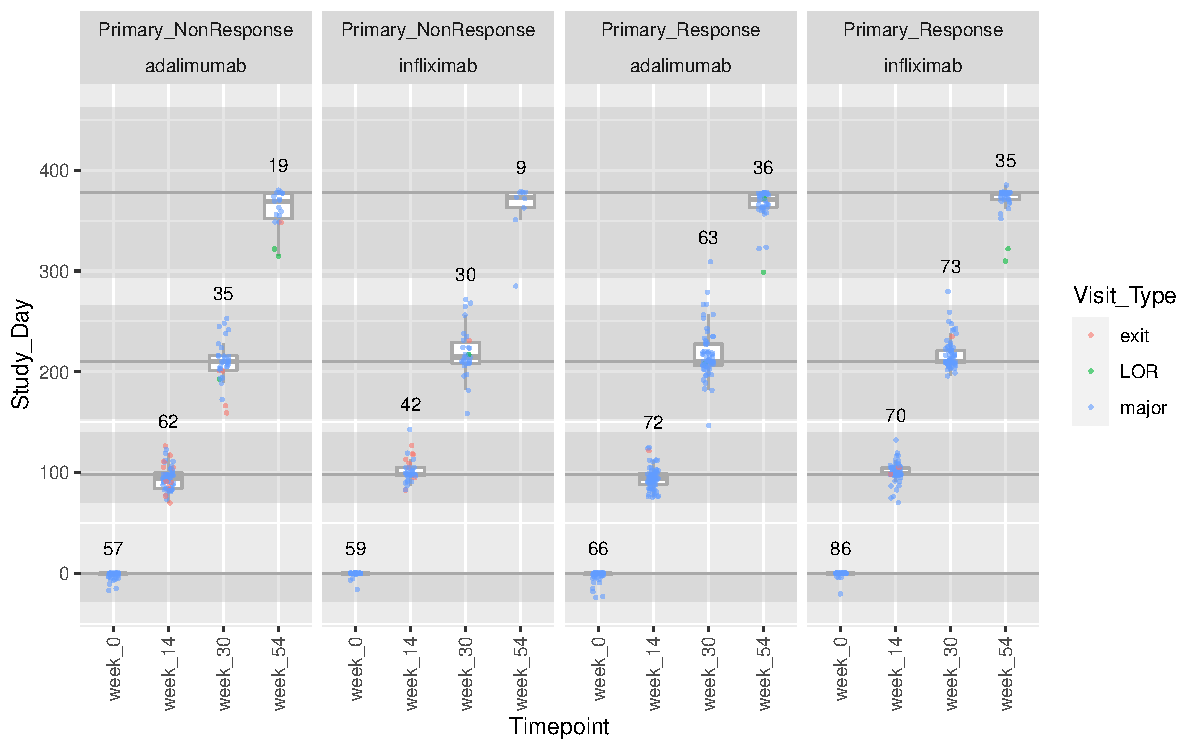
\includegraphics[width=1.0\textwidth,page=1]{mainmatter/figures/chapter_04/process_pheno.pheno_filtered_dge.Study_Day_vs_Visit_Label.pdf}
    \caption{
        \textbf{Number and sample day distribution for \gls{RNAseq} samples in each timepoint.}
        Windows for the four major visits are colored in grey. Samples mostly come from major visits, but a small number of \gls{LOR} and exit visit samples were included according to the criteria in \cref{subsubsec:multiPANTS_timepoints_def}.
    }
    \label{fig:multipants_studyDay_boxplots}
\end{figure}

\subsection{Definition of primary response and non-response}
\label{multiPANTS:PR_definition}

% "there is agreement that primary nonresponse to anti‐TNF drugs should not be assessed prior to 14 weeks following initial induction infusions with use of infliximab, or prior to 12 weeks for adalimumab injections" \autocite{dhaens2011LondonPositionStatement}
The definition of primary response and non-response was based on the clinical decision tree from \textcite{kennedy2019PredictorsAntiTNFTreatment}.
Primary response status was assessed at week 12, prior to the scheduled week 14 visit. 
The criteria for primary non-response was \emph{either} of the following: 
\begin{itemize}
    \item exit for treatment failure before week 14 (e.g. as decided by physician global assessment), \emph{or} corticosteroid use at week 14 (a continuing or new prescription);
    \item compared to week 0, a decrease in \gls{CRP} by less than 50\% or to >\SI{3}{\milli\gram\per\litre}, \emph{and} a decrease in \gls{HBI} by less than 3 points or to >4.
\end{itemize}
As \gls{PANTS} was an observational study that continued until drug withdrawal, a patient's clinician may have decided to continue anti-\gls{TNF} therapy even if a patient had primary non-response, so it was possible for non-responders to be sampled past week 14.
The criteria I used to define primary response\footnote{These are the criteria used by \textcite{kennedy2019PredictorsAntiTNFTreatment} to define week 14 remission.} was \emph{all} of the following:
\begin{itemize}
    \item not classified as a primary non-responder;
    \item \gls{CRP} \SI{\le 3}{\milli\gram\per\litre} by week 14;
    \item \gls{HBI} \SI{\le 4} by week 14.
\end{itemize}
Patients that only met a subset of criteria for either primary response or primary non-response were excluded.

% TODO: check this section. PNR is right, but PR is not  PNR is right, but PR is not "Response" on the flowchart, but "Remission"
% Selection criteria for samples from Nick:
%
% "~200 for each drug, ~100 PNR, 100 remission. PNR had to be PNR at week 14 and non-remission at week 54 (or unknown at week 54). 
% Remission had to have active disease at baseline and be in remission or response at week 14 and remission at week 54 (or unknown at week 54 and remission at week 30).
% ideal_downstream_cohort <- bd_vr_clin %>%
%   filter(
%     (crp_visit_1 >= 4 | calpro_visit_1 > 100),
%     (pnr & (is.na(remission_visit_5) | !remission_visit_5)) |
%     ((status_visit_2_3 %in% c("Response", "Remission")) & (remission_visit_5 | (is.na(remission_visit_5) & remission_visit_4)))
%   )
% They also had to be 16 years or over and have a baseline serum sample. 
% Within the infliximab patients, there was propensity matching between PNR/non-PNR based on on_imms_visit_1 + on_steroids_visit_1 + age_at_first_dose + earliest_weight_category_4 + albumin_visit_1 + sex."
There were additional inclusion criteria applicable to just the \gls{RNAseq} subcohort analyses in this chapter.
Patients were required to be at least 16 years old, and have an available baseline serum sample.
Primary non-responders were filtered to exclude patients in remission at week 54.

\subsection{Library preparation and \glsfmtshort{RNAseq}}

% From Mark:
% Here is an extended version of the protocol, with highlighting of the portion on poly-A selection and subsequent depletion steps:
%
% RNA and DNA were isolated from whole blood samples collected in Tempus Blood RNA Tubes.
%
% The Applied Biosystems Tempus Blood RNA Tube and Tempus Spin RNA Isolation kit was adapted to work in concert with the Qiagen QIAsymphony PAXgene Blood RNA (762635) and DNA DSP Midi (937255) Kit protocol for total RNA and DNA isolation from Tempus blood RNA tubes.
%
% Day 1: Batches of 48 tempus tubes were removed from -80°C and scanned into the electronic isolation record. Sample blood tube barcodes were matched to shipping barcodes and arranged by subject ID in visit order. Sample blood tubes were transferred to 4°C to thaw overnight. In preparation for DNA isolation, 48 14mL polystyrene culture tubes (BD352051) were labeled with Genomic Technologies barcodes and scanned into the electronic isolation record alongside the corresponding sample IDs.
%
% Day 2: Sample blood tubes were removed from 4°C and inverted 10 times to ensure efficient lysis. Samples were then left at room temperature to equilibrate for 2 hours. To obtain RNA and DNA from the same blood samples the following steps were performed: (1) Prepared the blood tube samples by following the Applied Biosystems manufacturer’s protocol “Processing Stabilized Blood before Purification” steps 1-5 (Nunc 50mL conical tubes 52000-004, PBS 1x -Ca2+ -Mg2+ pH 7.2 (20012050). After centrifugation, 2mL of the supernatant was aliquoted into the 14mL barcoded culture tubes for DNA isolation and placed in the 4°C until ready for the DNA isolation protocol with the Qiagen QIAsymphony DNA DSP Midi kit. The remaining supernatant was poured off of the RNA pellet and allowed to briefly dry. The blood samples then followed the Qiagen QIAsymphony PAXgene blood RNA manufacturer’s protocol at step 3. The following QIAsymphony instrument protocol was performed for isolation of Total RNA, RNA Isolation PAX RNA CR22332 ID 2915. The RNA samples were eluted in an 80uL volume and stored at -80°C, UltraPure DNase/RNase Free Distilled Water (10977023). The QIAsymphony was then loaded with the necessary reagents and consumables to perform the DNA isolation protocol. The DNA blood samples were removed from 4°C and loaded onto the QIAsymphony. The following QIAsymphony instrument protocol was performed for isolation of DNA, DNA isolation Blood_1000_V7-DSP. The DNA samples were eluted in a 200uL volume and stored at -80°C. RNA and DNA nucleic acid quantification were performed with the ThermoFisher QuBit BR RNA (Q10211) and QuBit BR dsDNA (Q32853) kits respectively, following the manufacturer’s protocol. RNA integrity analysis was performed with the Agilent RNA ScreenTape assay (5067-5579, 5067-5577, 5067-5576) on the Agilent 4200 TapeStation following the manufacturer’s protocol. Results were uploaded into the electronic isolation record and used RNA and DNA normalization.
%
% RNA library preparation from total RNA was conducted following the manufacturer’s protocol for the Kapa mRNA HyperPrep Kit. Briefly, 250 ng of total RNA was enriched for mRNA using magnetic oligo-dT beads. The remaining RNA was then fragmented by magnesium under elevated temperature. After fragmentation RNA was depleted of rRNA and globin mRNA using the QIAseq FastSelect RNA Removal Kit by Qiagen. The depleted RNA then underwent first strand synthesis using reverse transcriptase and random primers. Combined second strand synthesis and A-tailing incorporated dUTP into the second cDNA strand for stranded RNA sequencing and added dAMP to the 3’ ends for adapter ligation. The cDNA fragments were then ligated to sequencing adaptors (IDT xGEN Dual Index UMI adapters) and was enriched using 16 cycles of PCR. Final libraries were assessed using the Agilent Tapestation and Qubit (ThermoFisher) assay methods then sequenced on an Illumina HiSeq 4000 sequencer using 2x75bp read length.

Total RNA was extracted following the Qiagen QIAsymphony instrument protocol (RNA Isolation PAX RNA CR22332 ID 2915).
RNA was quantified with the ThermoFisher QuBit BR RNA (Q10211), 
and RNA integrity assessed with the Agilent RNA ScreenTape assay (5067-5579, 5067-5577, 5067-5576) on the Agilent 4200 TapeStation.

Library preparation was performed using the Kapa mRNA HyperPrep Kit, including enrichment for mRNA using magnetic oligo-dT beads, depletion of rRNA and globin mRNA using the QIAseq FastSelect RNA Removal Kit, and adapter ligation with IDT xGEN Dual Index UMI adapters.
Libraries were sequenced on the Illumina HiSeq 4000 with \si{75}{bp} paired-end reads.

\subsection{RNAseq quantification and preprocessing}

A total of 1141 samples from 396 patients were initially sequenced to a median depth of \textapprox{20} million read pairs.
Sequencing data was demultiplexed with Picard.
Total number of read pairs, sequence quality, overrepresented sequences, adapter content and sequence duplication rates were checked using FastQC.
% "To demultiplex and annotate the reads with the UMI information we use the Picard commands outlined in the attached file. We align using STAR (https://www.ncbi.nlm.nih.gov/pmc/articles/PMC3530905/ [ncbi.nlm.nih.gov]), mark and remove duplicates using UMITools (https://github.com/CGATOxford/UMI-tools [github.com]), and get our gene counts using featureCounts (http://subread.sourceforge.net/ [subread.sourceforge.net]). For QC we use fastQC, Picard, and compile the results together using MultiQC."
%
% "With the UMI protocol, raw fastq files are generated per sample/per lane, so there are 8 files per sample and they don’t actually contain the UMI information, so they are probably not ideal for starting your work. We should speak about where along the pipeline you are comfortable with us sending you the PANTS RNAseq
% Roughly the pipeline:
% Raw .bcl files -> demultiplexed unaligned .bam file per sample/per lane (8 files per sample) ->  fastq without UMI information per sample/per lane -> alignment -> aligned .bam files without UMI information per sample/per lane -> merge aligned .bam with unaligned .bam including UMI information -> merge .bam files for a sample across lane (1 file per sample) -> mark duplicates using UMIs -> create deduplicated .bam file -> create counts matrix and run QC -> optional creation of fastq files with UMIs in read names
Reads were mapped to GRCh38 using STAR (2.6.1d) and deduplicated to unique reads using UMI-tools.
Gene expression was quantified against the Ensembl 96 gene annotation with featureCounts (1.6.4).

Samples were filtered to remove outliers (\num{>2} standard deviations from the mean) according to percentage of aligned reads in coding regions reported by Picard, percentage of unique reads, and number of unique reads.
Samples that could not be mapped to a timepoint according to \cref{subsubsec:multiPANTS_timepoints_def} were removed.
Samples that came from patients with 
sex mismatch,
% based on Y chromosome gene expression,
grey zone primary response, 
or missing data for variables considered in the variable selection process (\cref{subsubsec:multiPANTS_var_selection}),
were removed.
A total of 814 samples remained after filtering.
The number of samples mapping to each timepoint as defined in \cref{subsubsec:multiPANTS_timepoints_def} is shown in \cref{fig:multipants_studyDay_boxplots}.
The number of samples per patient ranged from one to four, with a median of three (\cref{fig:multipants_visits_upset}).

\begin{figure}
    \centering
    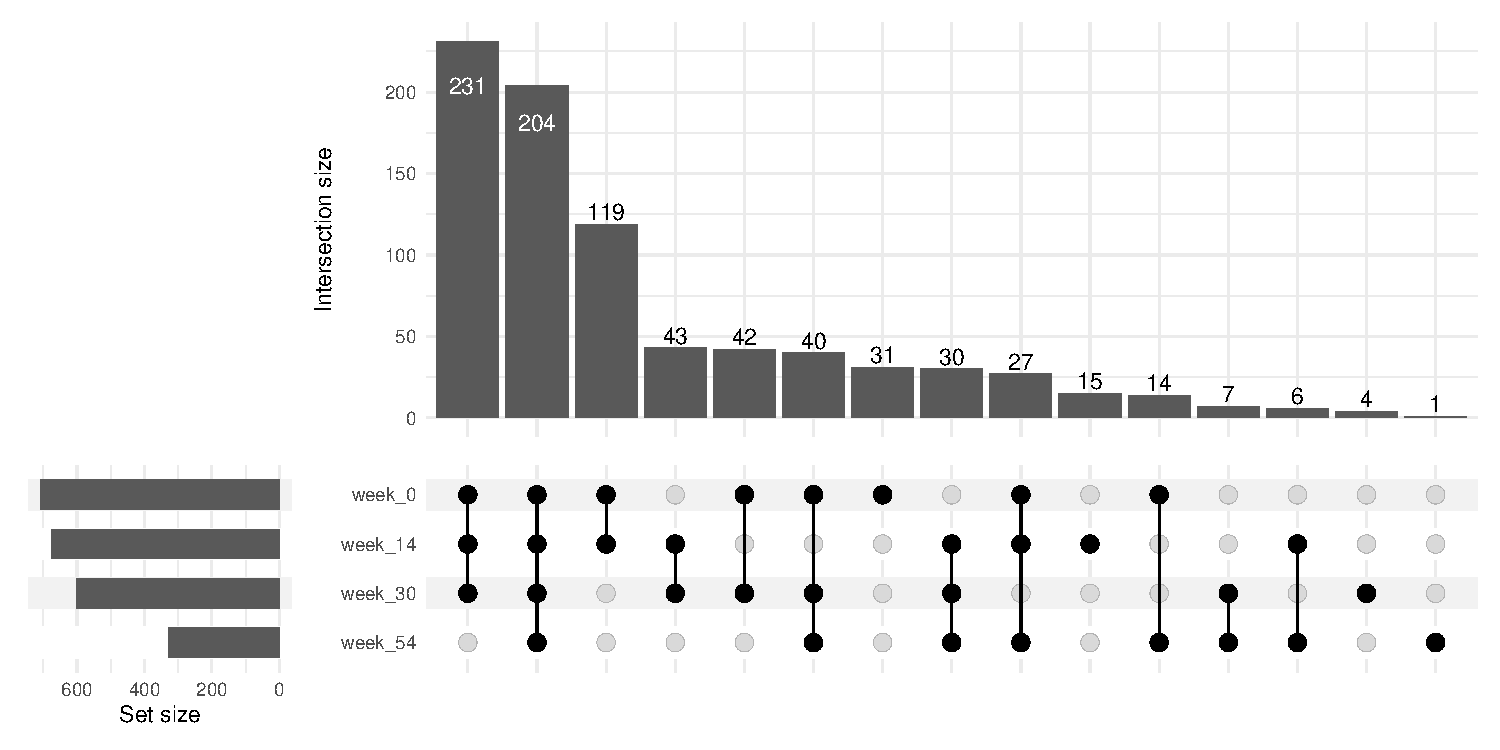
\includegraphics[width=1.0\textwidth,page=1]{mainmatter/figures/chapter_04/process_pheno.pheno_filtered_dge.Visit_Label_upset.pdf}
    \caption{
        \textbf{Distribution of \gls{RNAseq} samples from each patient among timepoints.}
    }
    \label{fig:multipants_visits_upset}
\end{figure}

The Ensembl 96 gene annotation contains \SI{58884} genes, many of which are not expressed in whole blood.
Effective library sizes were computed using the \gls{TMM} method in \software{edgeR} \autocite{robinson2010EdgeRBioconductorPackage}.
Between-sample normalisation for library size was performed using \software{edgeR::cpm}, converting counts to \gls{CPM}.
Genes with low expression were filtered,
requiring >1.25 CPM in >10\% of samples (1.25 \gls{CPM} was approximately 10 counts at the median library size of 8 million unique mapped read pairs),
and non-zero expression in >90\% of samples.
% NOTE: probably don't need to remove these manually in future.
Globin genes and short \glspl{ncRNA} were removed.
A total of \num{15511} genes remained after filtering.
Finally, \glspl{CPM} were converted to the $\log_{2}$ scale, and precision weights to account for the expression mean-variance relationship were computed for each gene and sample using \software{voomWithDreamWeights} from \software{variancePartition} \autocite{hoffman2016VariancePartitionInterpretingDrivers}.

\subsection{\Glsfmtlong{DGE}}

\subsubsection{Variable selection by variance components analysis}
\label{subsubsec:multiPANTS_var_selection}

% TODO: arrows are directed causal effects, so remove these if talking about association
For each gene, the \gls{DGE} model was a regression expressing the response variable, gene expression, 
as a linear function of predictor variables of interest (primary response status, drug, timepoint),
and other selected predictor variables.
In estimating the association of predictor X to response Y by regression, 
adjustment for a third variable Z can increase, decrease, or even reverse the effect estimate of X (the regression coefficient).
I aimed to select third variables for inclusion into the \gls{DGE} model that were covariates,
defined here as a Z that is associated with Y, but not with X.
Such variables are also known as neutral controls \autocite{cinelli2020CrashCourseGood}, precision variables, or prognostic variables,
At the cost of 1 \gls{df},
Z explains variation in Y that would otherwise be considered residual,
so conditioning on Z increases the efficiency of estimating the effect of X on Y, but does not change the effect estimate.

Many variables were available for selection;
\cref{fig:multipants_pheno_filtered_ggcorrplot} shows their correlation matrix.
% Univariable analyses showed the strongest associations with primary non-response to infliximab and adalimumab were with week 14 drug and anti-drug antibody concentrations (table 3; appendix p 17).
% Primary non-response to infliximab was also associated with older age at first dose, smoking at baseline, non-use of an immunomodulator at baseline, lower baseline albumin concentrations, and higher baseline white cell count.
% Primary non-response to adalimumab was associated with a higher body-mass index at baseline.
These included three variables associated with primary response in \textcite{kennedy2019PredictorsAntiTNFTreatment}: baseline immunomodulator use, smoking and \gls{BMI}.
% From Mark:
% As a follow-up, here is what Sam shared about estimating cell composition in the data: “We used the Houseman method [bmcbioinformatics.biomedcentral.com], which is implemented with the estimateCellCounts() function from the minfi package in R.”
Also available were proportions of six common cell types in whole blood 
(CD4\textsuperscript{+} T cells, CD8\textsuperscript{+} T cells, B cells, \gls{NK} cells, monocytes, granulocytes),
estimated using the Houseman method (\software{minfi::estimateCellCounts} \autocite{aryee2014MinfiFlexibleComprehensive})
from whole blood Illumina MethylationEPIC methylation array data collected from the same patients and timepoints.
The Houseman method uses differentially methylated regions between immune cell types as cell type markers \autocite{houseman2012DNAMethylationArrays}.

% TODO: labels here don't match listings
\begin{figure}
    \centering
    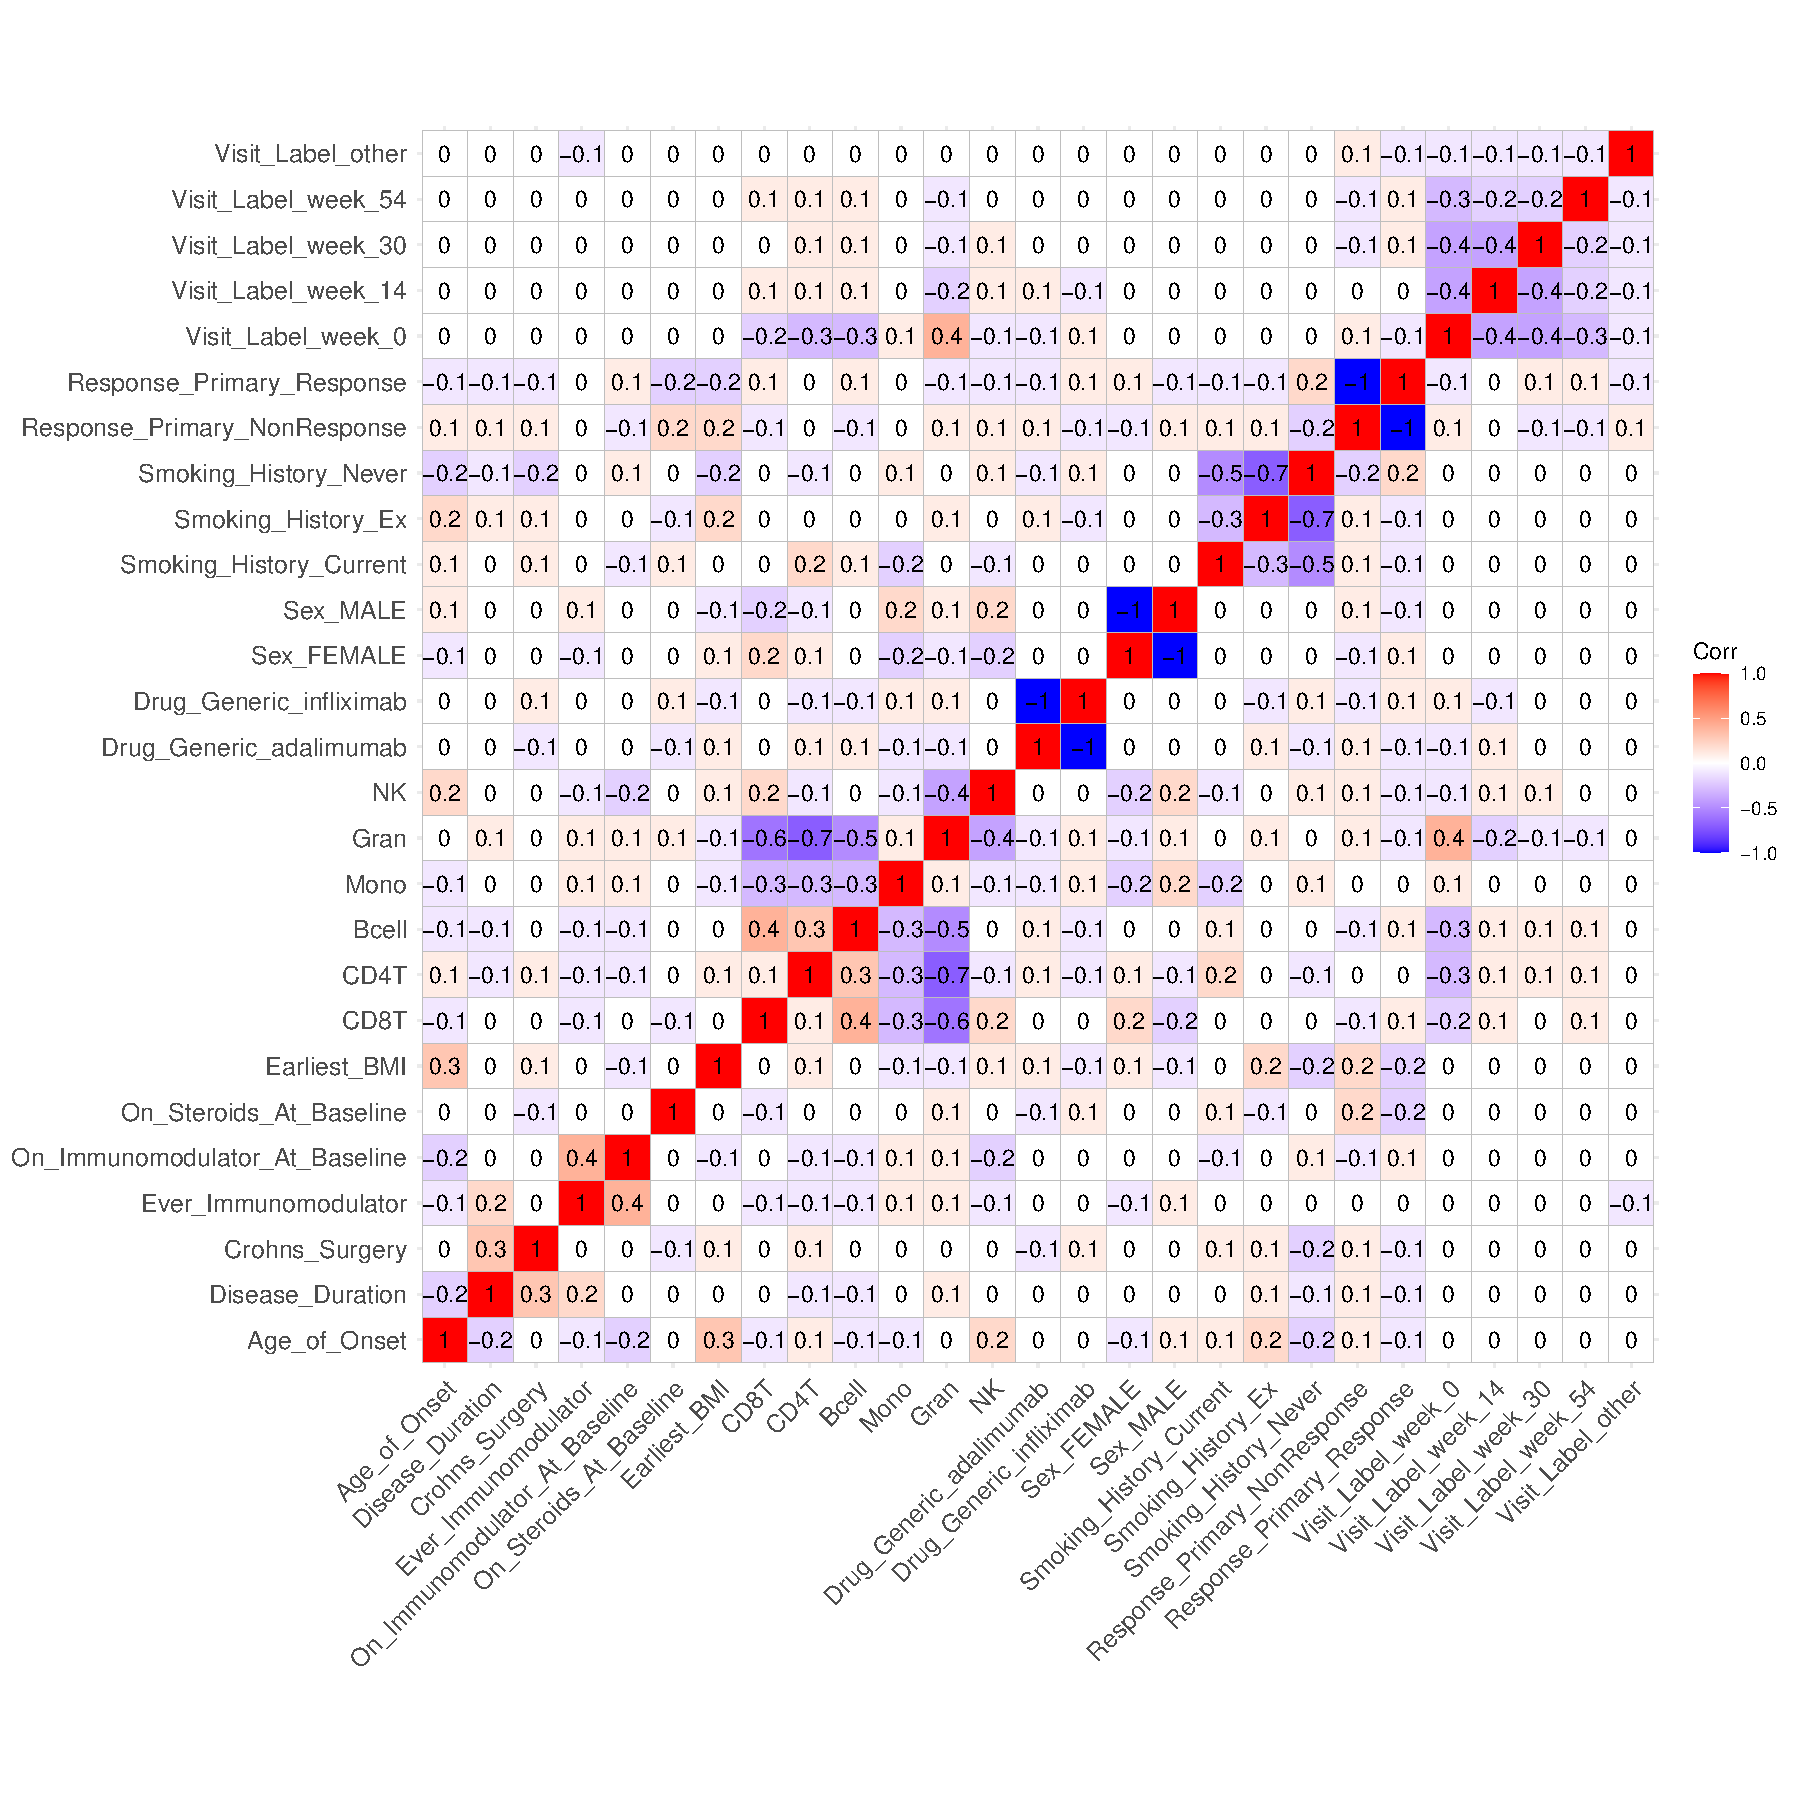
\includegraphics[width=1.0\textwidth,page=1]{mainmatter/figures/chapter_04/process_pheno.pheno_filtered_dge.ggcorrplot.pdf}
    \caption{
        \textbf{Correlation matrix of variables measured in \gls{PANTS} that were considered as potential independent variables.}
        NK = \gls{NK} cell, Gran = granulocyte, Mono = monocyte, Bcell = B cell, CD4T = CD4+ T cell, CD8 = CD8+ T cell.
    }
    \label{fig:multipants_pheno_filtered_ggcorrplot}
\end{figure}

% \1 Visualised main factors that influence global gene expression by PCA (\cref{fig:multipants_dream_prcomp})
%     \2 main separation along PC1 is w0 anti-TNF naive samples from all other post-drug start samples

% \begin{figure}
%     \centering
%     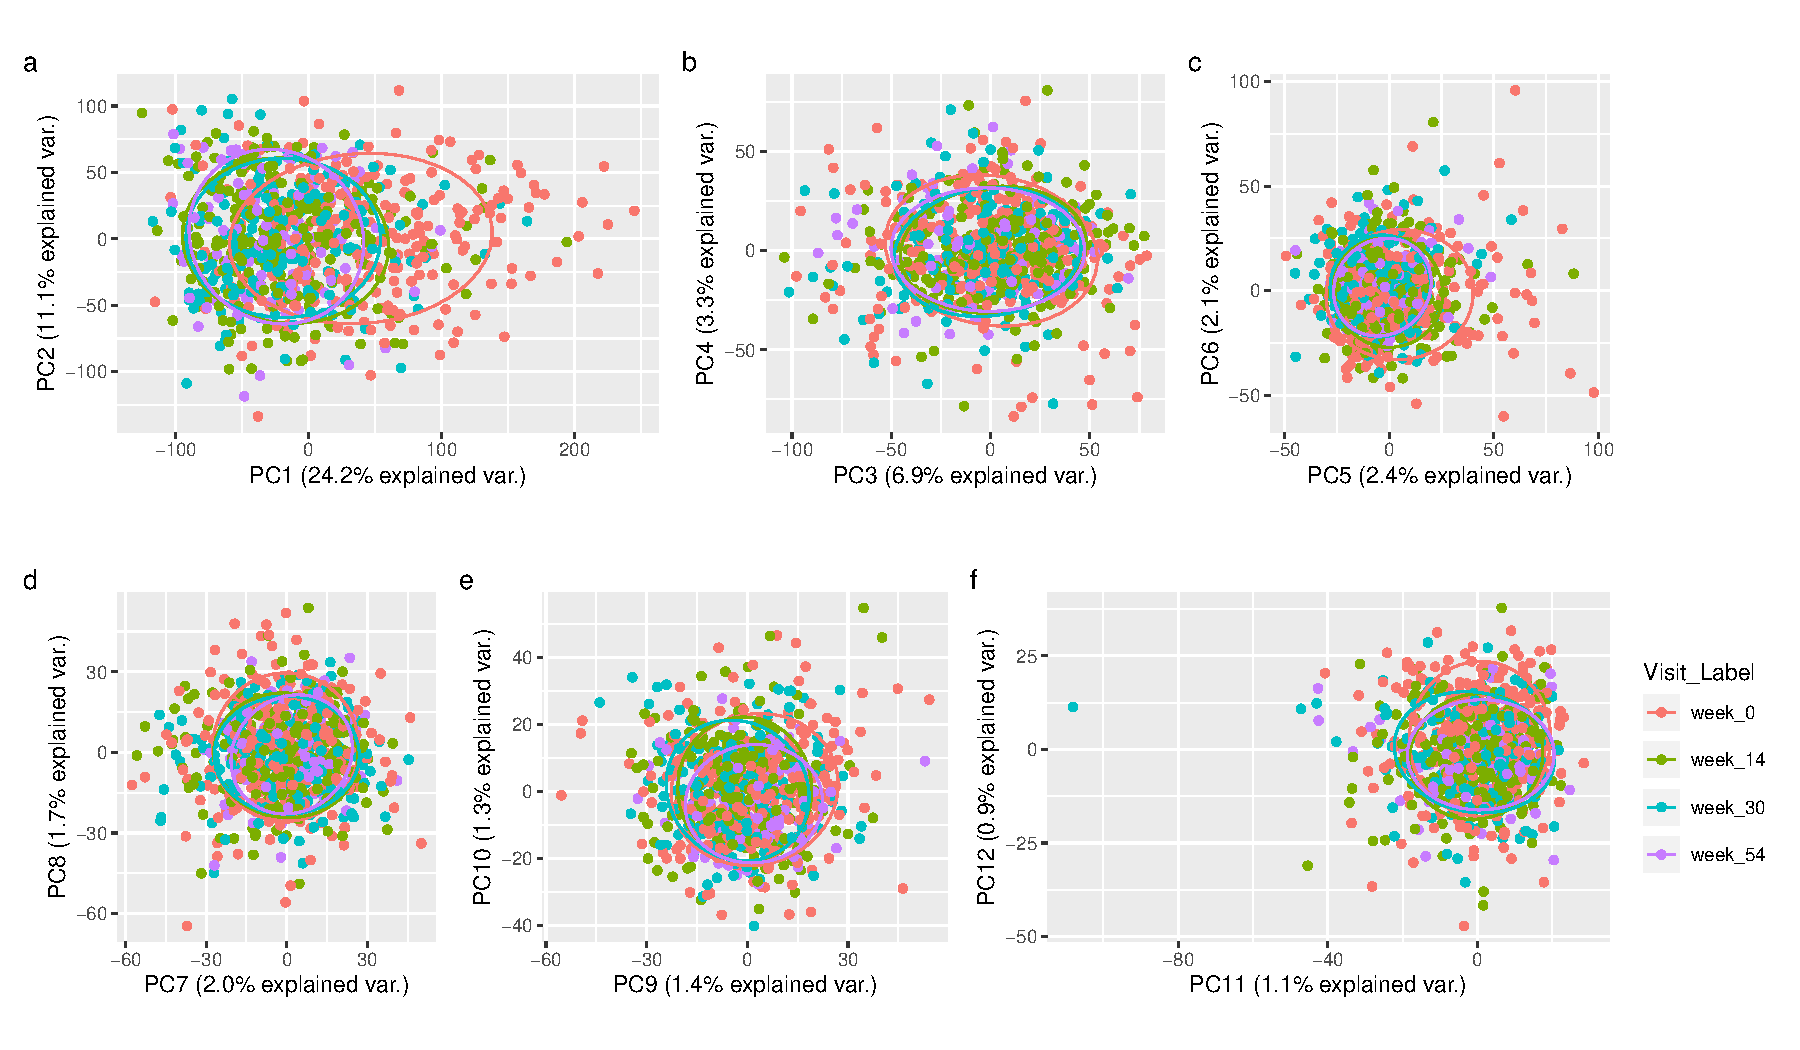
\includegraphics[width=1.0\textwidth,page=1]{mainmatter/figures/chapter_04/dream.prcomp.pdf}
%     \caption{top 12 expression PCs of filtered expression data}
%     \label{fig:multipants_dream_prcomp}
% \end{figure}

A variance components analysis was performed to quantify the proportion of expression variance explained by each variable for each gene using \software{variancePartition} \autocite{hoffman2016VariancePartitionInterpretingDrivers}.
Variables that do not explain much variation in the response are unlikely to improve efficiency if conditioned on.
The model was a mixed effects regression model with variables in \cref{fig:multipants_pheno_filtered_ggcorrplot} included as predictors.
Additional categorical variables were included for patient and \gls{RNAseq} library preparation plate.
An additional continuous variable consisting of random numbers drawn from the standard normal distribution was also included as a null.
% The var explained by Gran will be redistributed among highly cor vars anyways.
Granulocyte proportion estimates were dropped to relieve perfect multicollinearity.
Categorical variables were coded as random intecepts, and continuous variables as fixed effects.
Surprisingly, simulations from \textcite{hoffman2016VariancePartitionInterpretingDrivers} showed variance proportion estimates were unbiased even when coding categorical variables with as few as two categories as random effects. 
This was the case as long as model parameters were estimated using \gls{ML} rather than \gls{REML}. 
% which is commonly used for variance components analysis.
It was also shown this approach avoids overestimates of variance proportions that occur if categorical variables with many levels are treated as fixed.

As downstream \gls{DGE} methods require the same set of predictors for all genes, the aim was to select variables that explain a lot of variance for many genes.
Variables that explained the most variance on average were patient, cell proportions and \gls{RNAseq} plate (\cref{fig:multipants_varPart}).
Some variables that did not explain more variance on average than the null nevertheless had high maximum values, indicating their importance for a relatively small number of genes.
These included sex, library preparation protocol version, and smoking status.
However primary response status---a variable of interest---also fell into this group,
so it was difficult to justify excluding all variables with lower median variance explained than the null.
Consequently, all non-null variables in \cref{fig:multipants_varPart} were selected as predictors in downstream models apart from \enquote{Ever\_Immunomodulator} 
(whether the patient had ever had immunomodulator treatment), 
as that variable had both low median variance explained and was correlated with baseline immunomodulator use.
This is a crude approach, but the sample size is large compared to number of \glspl{df} lost by including predictors that may not be relevant for some genes.
% TODO: check robustness of DGE results to predictor set

\begin{figure}
    \centering
    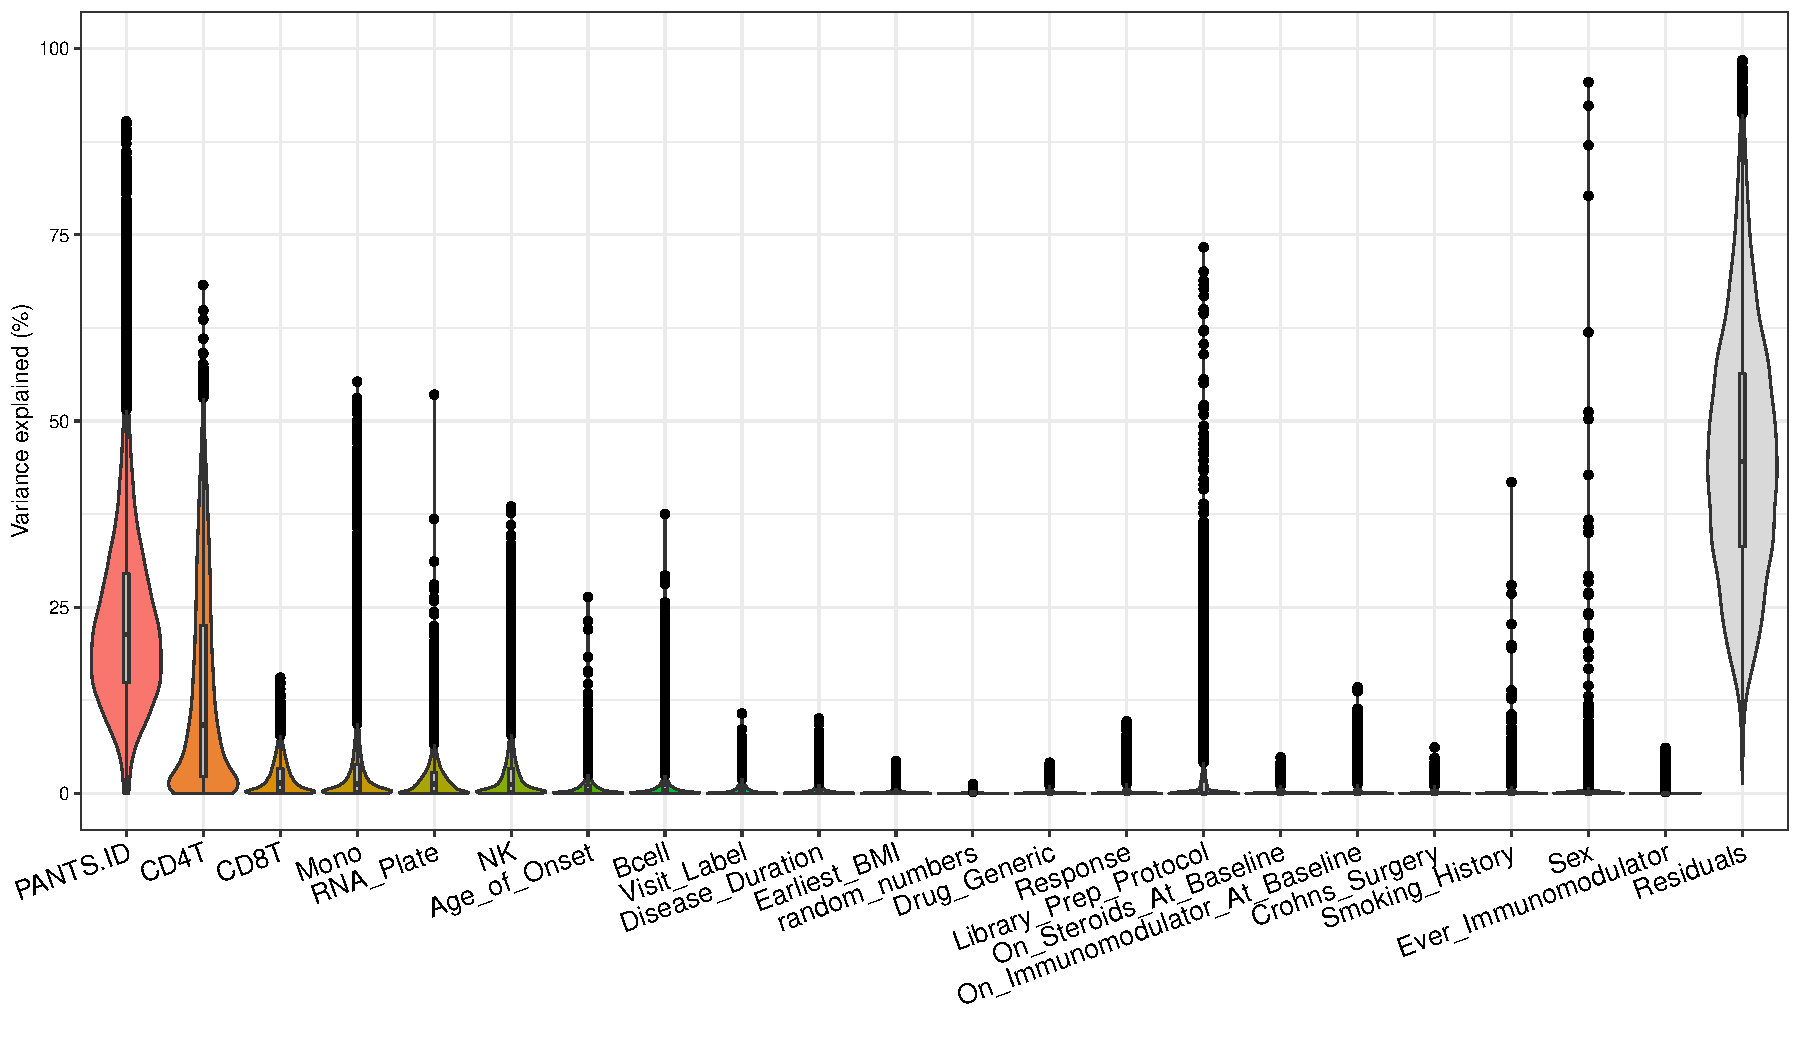
\includegraphics[width=1.0\textwidth,page=1]{mainmatter/figures/chapter_04/dream.plotVarPart.pdf}
    \caption{
        \textbf{Variance components analysis showing distribution of per-gene percentage of variance in expression explained by each variable.}
        Variables are ordered by the median of per-gene variance proportion estimates.
        random\_numbers is the null, drawn from the standard normal distribution.
        PANTS.ID = patient ID, NK = \gls{NK} cell, Gran = granulocyte, Mono = monocyte, Bcell = B cell, CD4T = CD4+ T cell, CD8 = CD8+ T cell.
}
    \label{fig:multipants_varPart}
\end{figure}

How might interpretations of effect sizes of interest be affected by including this suite of other variables, all of which can be considered as third variables?
If a third variable Z is not a precision variable, but is also associated with X, conditioning changes the effect estimate.
The regression model is mathematically agnostic to causal relationships between variables,
but distinct types of third variable can be distinguished conceptually by assuming the direction of causal relationships \autocite{mackinnon2000EquivalenceMediationConfounding}.
Conditioning on a confounder ($X \leftarrow Z \rightarrow Y$) reduces bias of the effect estimate,
conditioning on a collider ($X \rightarrow Z \leftarrow Y$) induces bias,
and conditioning on a mediator in the causal path ($X \rightarrow Z \rightarrow Y$) changes the effect estimated by removing the indirect effect mediated by Z,
usually biasing the effect estimate towards zero\footnote{It is not easy to determine the direction of bias (positive or negative) for any of these cases in general \autocite{suzuki2020CausalDiagramsPitfalls}.}.

From the variance partition analysis (\cref{fig:multipants_varPart}), cell proportions were among the biological factors that explained the most variance on average,
they are one of the largest sources of variation in bulk blood expression data, 
and are a major driver of immune response to perturbations \autocite{piasecka2018DistinctiveRolesAge}.
% They change a lot over time too (\cref{fig:multipants_cell_type_proportion_vs_Study_Day})
Thus I decided to I fit two sets of separate \gls{DGE} models including and excluding cell proportions as predictors, but otherwise identical.
Assuming that cell proportions act as a mediator of the drug's effect on gene expression, these models have complementary interpretations.
In models without cell proportions included, differential expression after drug perturbation could represent up or downregulation on a per cell basis, 
but could also come from differences in cell proportions induced by the drug.
The estimates from models adjusted for cell proportions are more likely to reflect up or downregulation on a per cell basis.
% \todo{Could cell proportions act as colliders?}
When comparing expression between responders and non-responders,
one might also assume cell proportions can mediate the effect of a patient's response status on expression%
\footnote{
    The assumption that response status is a stable property of a patient that can be treated as an independent variable will be discussed in \cref{sec:discussion_responderAnalysis}.
}.
Analogously, estimates of expression differences between responders and non-responders from the two sets of models 
also have complementary interpretations: total difference, and per-cell differences not due to differences in cell proportions.
Throughout this chapter, I interpret the estimates from both sets of models accordingly.

% \begin{figure}
%     \centering
%     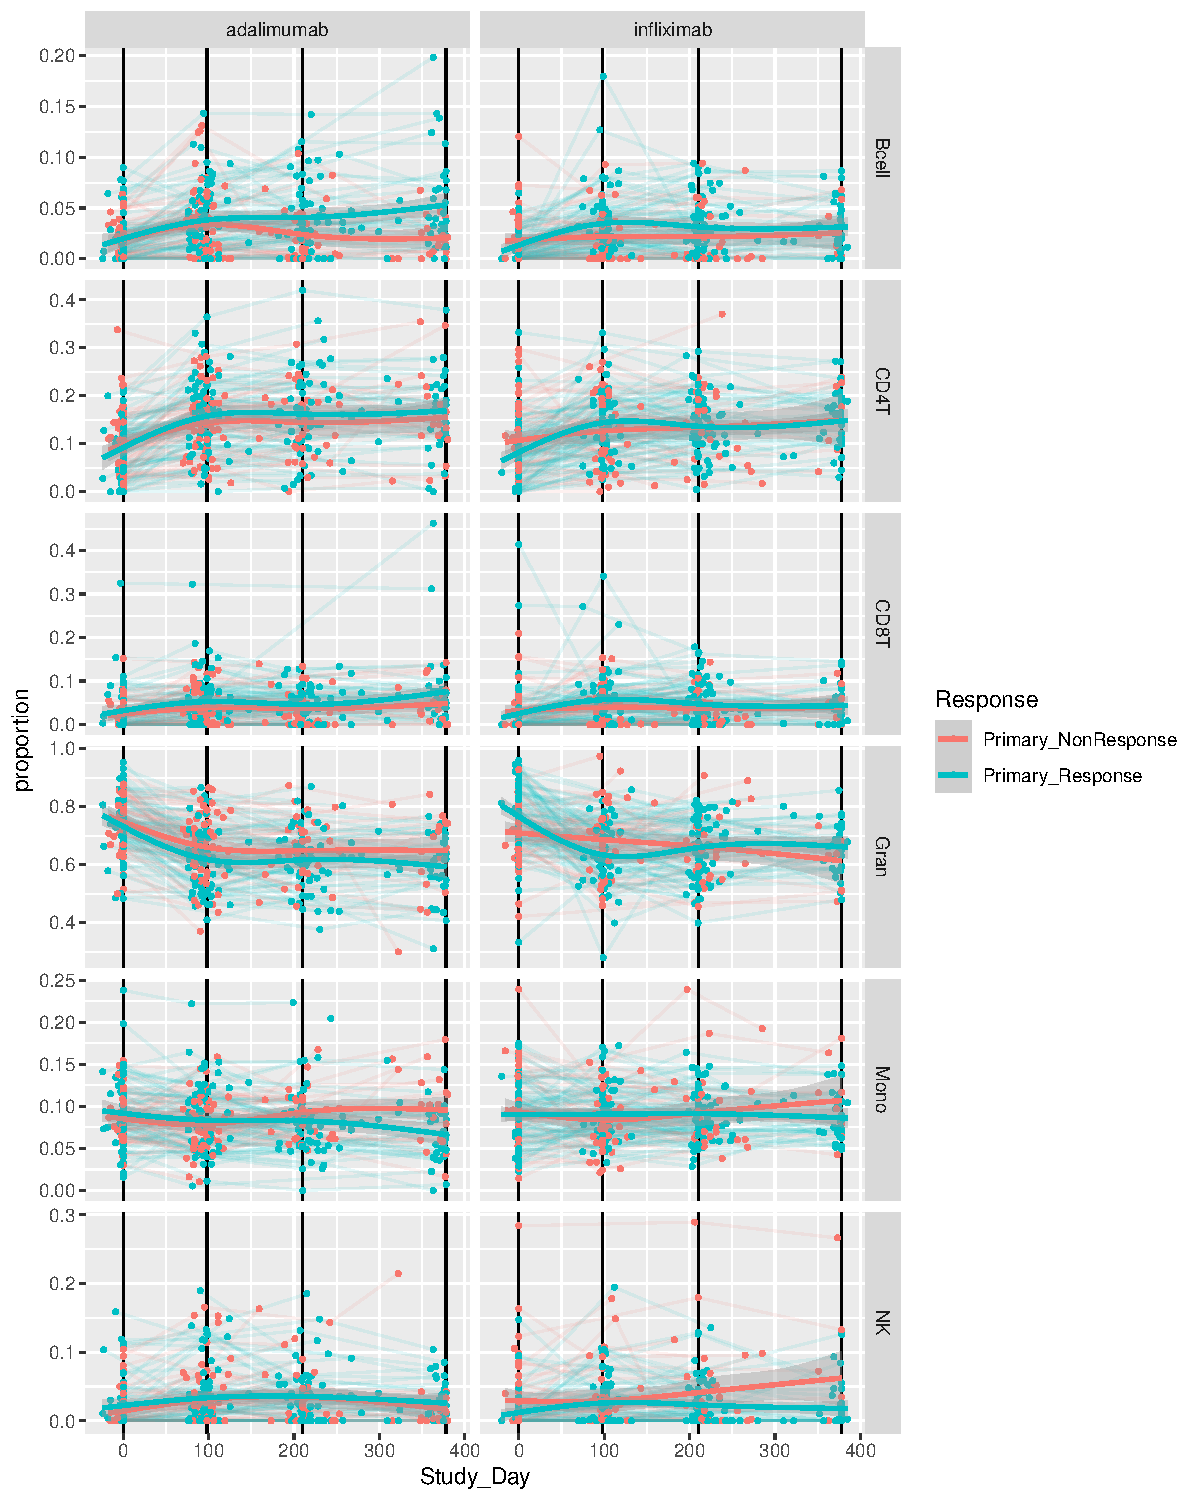
\includegraphics[width=1.0\textwidth,page=1]{mainmatter/figures/chapter_04/dream.cell_type_proportion_vs_Study_Day.pdf}
%     \caption{changes in cell proportions of 6 immune cell types over time}
%     \label{fig:multipants_cell_type_proportion_vs_Study_Day}
% \end{figure}

\subsubsection{Contrasts for pairwise group comparisons}

Per-gene \gls{DGE} models were fit in \software{dream} \autocite{hoffman2020DreamPowerfulDifferential}.
Like the variance partition model models, these \gls{DGE} models were linear mixed models:
%
% \begin{lstlisting}
% Expression ~
%     0 +
%     concat(Visit, Response, Drug) +
%     Sex + Age_of_Onset + Disease_Duration +
%     Smoking_History + Crohns_Surgery +
%     On_Immunomodulator_At_Baseline +
%     On_Steroids_At_Baseline + Earliest_BMI +
%     [CD8T + CD4T + Bcell + Mono + NK] +
%     Library_Prep_Protocol +
%     (1 | RNA_Plate) +
%     (1 | Patient)
% \end{lstlisting}
%
\begin{equation}
y = 0 + \beta_{trd} G_{trd} + \sum_{}^{9}{\beta_Z Z} + (\sum_{}^{5}{\beta_C C}) + u + v + \epsilon
\label{eq:multiPANTS_dge_model}
\end{equation}
where:
\begin{itemize}
    \item the response variable is gene expression $y$.
    \item 0 indicates there is no intercept term.
    \item $G_{trd}$ is a fixed effect for experimental group defined by combinations of the predictors of interest:
        timepoint (week 0, 14, 30, 54), 
        response (responder, non-responder), 
        and drug (infliximab, adalimumab).
        This is equivalent to having an intercept term and a three-way interaction between visit, response, and drug, including all lower order terms,
        but is more convenient for testing pairwise expression differences between groups,
        as the coefficient for each term is the estimate of mean expression for that group.
        % TODO: move variable descriptions up
    \item $\sum_{}^{9}{\beta_Z Z}$ are the non-cell proportion fixed effects chosen in \cref{subsubsec:multiPANTS_var_selection}:
        sex (Sex), 
        age of disease onset (Age\_of\_Onset), disease duration (Disease\_Duration), 
        smoking history (Smoking\_History: ex, current or never), 
        whether the patient has had surgery for \gls{CD} (Crohns\_Surgery), 
        whether the patient was on immunomodulator at baseline (On\_Immunomodulator\_At\_Baseline), 
        whether the patient was on steroids at baseline (On\_Steroids\_At\_Baseline), 
        \gls{BMI} at baseline (Earliest\_BMI),
        and library preparation protocol version (Library\_Prep\_Protocol).
    \item $\sum_{}^{5}{\beta_C C}$ are the cell proportion fixed effects chosen in \cref{subsubsec:multiPANTS_var_selection},
        for \gls{NK} cells, monocytes, B cells, CD4+ T cells, and CD8+ T cells.
    \item $u$ is a random intercept for \gls{RNAseq} plate (RNA\_Plate).
    \item $v$ is a random intercept for patient (PANTS.ID), nested inside \gls{RNAseq} plate.
\end{itemize}

As the interest was in estimating a single coefficient for each predictor's effect size on expression (rather than estimating variance components), 
most predictors above are modelled as fixed effects.
Since \gls{RNAseq} plate and patient are nuisance variables with a large number of levels they are modelled as random intercepts.
A total of four sets of per-gene models were fit,
with and without the cell proportion terms $\sum_{}^{5}{\beta_C C}$,
and replacing $\beta_{trd} G_{trd}$ (separate drug models) with $\beta_{tr} G_{tr} + \beta_d d$ (pooled drug models) or not.
% https://web.stanford.edu/class/psych252/section/Mixed_models_tutorial.html#reml-vs.ml
% You should use ML when comparing models that differ in their fixed effects
% [...]
% In REML (REstricted ML) estimation, our main interest is in estimating the random effects, not the fixed effects.
% Imagine that we restrict our parameter space by setting the fixed effects parameters in set (i) above to certain plausible values.
% [...]
% it should not be used to compare models that differ in their fixed effects structure. You should just use this when comparing models that differ in their random effects.
%
% \gls{REML} treats fixed effects as nuisance parameters and estimates random effects after first integrating out fixed effects \autocite{mcneish2017SmallSampleMethods}.
As we are no longer performing variance components analysis,
to avoid small-sample bias in estimates of fixed effect standard errors, \gls{REML} was used for estimation \autocite{mcneish2017SmallSampleMethods}.

Specific hypotheses were tested using sum-to-zero contrasts, which are linear combinations of the model coefficients with weights summing to zero.
For example, 
to test for \gls{DGE} between responders and non-responders to infliximab at baseline in the non-pooled model,
I used a contrast where
the weight for the (week 0, responder, infliximab) group coefficient was 1,
the weight for the (week 0, non-responder, infliximab) group coefficient was -1,
and all other coefficient weights were 0.
% Contrasts can be used thuswise to compare any pair of groups, as the coefficients of group terms are group means.
%
% However, in the lme4 package in R the standards for evaluating significance of
% fixed effects in these models (i.e., obtaining p-values) are somewhat vague.
% There are good reasons for this, but as researchers who are using these models
% are required in many cases to report p-values, some method for evaluating the
% significance of the model output is needed.
%
% The primary motivation for this omission is that in linear mixed models it is
% not at all obvious what the appropriate denominator degrees of freedom to use
% are, except perhaps for some simple designs and nicely balanced data.
% 
% \2 to get p values for papers, Dream uses lmerTest approximation Satterthwaite df with REML
% \2 this combo controls type 1 error for n>144 in lmerTest simulations \url{https://link.springer.com/article/10.3758/s13428-016-0809-y}
To get \pvalues{}, the contrast divided by its standard error was compared to the $t$-distribution using the Satterthwaite approximation for \glspl{df}.
% \2 FDR BH separately per comparison: "The default method="separate" and
% adjust.method="BH" settings are appropriate for most analyses.
% method="global" is useful when it is important that the same t-statistic
% cutoff should correspond to statistical significance for all the
% contrasts." \url{https://rdrr.io/bioc/limma/man/decideTests.html}
\Gls{FDR} was controlled with the \gls{BH} method, threshold set at 0.05, computed separately for each contrast\footnote{
It could also have been computed globally over all contrasts if it were necessary to have the same $t$-statistic threshold for statistical significance in all contrasts.
}.

% NOTE: to get confidence intervals for FDR https://bmcbioinformatics.biomedcentral.com/articles/10.1186/1471-2105-12-288
% https://en.wikipedia.org/wiki/False_coverage_rate

\subsubsection{Spline model of expression over time}

% NOTE: there are tailored methods for time series DGE, but I did not use them due to shortness of this time series
% "Comparative analysis of differential gene expression tools for RNA sequencing time course data"
% Surprisingly, TC tools were outperformed by the classical pairwise comparison approach on short time series (<8 time points) in terms of overall performance and robustness to noise, mostly because of high number of false positives, with the exception of ImpulseDE2.
% Also see:
% Clustering time-course Microarray data using functional Bayesian infinite mixture model
% clustering folder in downloads
% https://2-bitbio.com/2017/04/clustering-rnaseq-data-making-heatmaps.html
% https://hbctraining.github.io/DGE_workshop/lessons/08_DGE_LRT.html

The aim was to use expression data from all four timepoints to find genes associated with response,
while avoiding a large number of pairwise comparisons.
I fit a natural cubic spline (\software{splines::ns}) to the study day to allow for non-linear trajectories of expression over time.
A cubic spline is a continuous function defined piecewise in each successive interval between a set of $k$ knots in the range of the input variable.
The $k-1$ pieces between knots are polynomials of degree 3. 
For a natural spline, the function is constrained to be linear outside of the boundary (first and last) knots to avoid unpredictable behaviour at the boundaries \autocite{perperoglou2019ReviewSplineFunction}.
%
% \begin{lstlisting}
% Expression ~
%      1 +
%      Primary_Response * ns(Study_Day, knots=7*c(14, 30)) +
%      Drug_Generic +
%      Sex + Age_of_Onset + Disease_Duration +
%      Smoking_History + Crohns_Surgery +
%      On_Immunomodulator_At_Baseline +
%      On_Steroids_At_Baseline + Earliest_BMI +
%      [CD8T + CD4T + Bcell + Mono + NK] +
%      Library_Prep_Protocol +
%      (1 | RNA_Plate) +
%      (1 | PANTS.ID)
% \end{lstlisting}
%
I set two inner knots at week 14 and week 30, as expression is expected to change after each drug dose.
To include all data to within the boundaries, the two boundary knots were set at the minimum and maximum values of study day rather than week 0 and week 54.
% "Function ns() from package splines indeed implements a natural cubic spline (aka restricted cubic spline) but using a B-splines basis representation. This provides an equivalent fit but it is not the same as the expansion you wrote in math. This expansion is implemented in function rcs() from the package rms."
% The function ns(Study\_Day, knots=7*c(14, 30)) returns a basis matrix for the spline with 3 \gls{df} (3 columns).
A basis matrix \autocite{perperoglou2019ReviewSplineFunction} was computed with \software{ns(Study\_Day, knots=7*c(14, 30))},
which is a matrix with 3 columns, each column being a transformation of the input, study day.
The columns are fit in the regression model in place of study day to allow for non-linear effects of study day on expression.
The model form used was as in \cref{eq:multiPANTS_dge_model},
except with $\beta_{trd} G_{trd}$
replaced by $\beta_r r + \sum_{}^{3}{\beta_b b} + \sum_{}^{3}{\beta_{rb} rb} + \beta_d d$,
where $r$ is response status,
$\sum_{}^{3}{\beta_b b}$ are the three columns of the basis matrix,
and $\sum_{}^{3}{\beta_{rb} rb}$ are the second-order interaction terms between response status and the basis matrix columns.
Separate sets of per-gene models were again fit with and without cell proportions $\sum_{}^{5}{\beta_C C}$.

% NOTE: true for poly, not true for ns
% https://stackoverflow.com/questions/19484053/what-does-the-r-function-poly-really-do
% Unfortunately there is an undesirable aspect with ordinary polynomials in regression. If we fit a quadratic, say, and then a cubic the lower order coefficients of the cubic are all different than for the quadratic [...]
% What we would really like is to add the cubic term in such a way that the lower order coefficients that were fit using the quadratic stay the same after refitting with a cubic fit. To do this take linear combinations of the columns of poly(horsepower, 2, raw = TRUE) and do the same with poly(horsepower, 3, raw = TRUE) such that the columns in the quadratic fit are orthogonal to each other and similarly for the cubic fit. That is sufficient to guarantee that the lower order coefficients won't change when we add higher order coefficients.
% [...]
% Importantly, since the columns of poly(horsepwer, 2) are just linear combinations of the columnns of poly(horsepower, 2, raw = TRUE) the two quadratic models (orthogonal and raw) represent the same models (i.e. they give the same predictions) and only differ in parameterization.
%
% http://www.science.smith.edu/~jcrouser/SDS293/labs/lab12-r.html
% This syntax fits a linear model, using the lm() function, in order to predict wage using a fourth-degree polynomial in age: poly(age,4). The poly() command allows us to avoid having to write out a long formula with powers of age. The function returns a matrix whose columns are a basis of orthogonal polynomials, which essentially means that each column is a linear combination of the variables age, age^2, age^3 and age^4.
% If we prefer, we can also use poly() to obtain age, age^2, age^3 and age^4 directly. We can do this by using the raw = TRUE argument to the poly() function. Later we see that this does not affect the model in a meaningful way -- though the choice of basis clearly affects the coefficient estimates, it does not affect the fitted values obtained.

To test for response-associated differences in the spline parameters, 
the predictors of interest are the interaction terms $\sum_{}^{3}{\beta_{rb} rb}$. 
% TODO F-test to p value
% f-test, is basically a wald test
% https://support.bioconductor.org/p/6124/
% The above mentioned statistics are computed for every contrast for each gene.
% The eBayes() function computes one more useful statistic. The
% moderated F-statistic (F) combines the t-statistics for all the
% contrasts for each gene into an overall test of significance for that
% gene. The moderated F-statistic tests whether any of the contrasts
% are non-zero for that gene, i.e., whether that gene is differentially
% expressed on any contrast. The moderated-F has numerator degrees of
% freedom equal to the number of contrasts and denominator degrees of
% freedom the same as the moderated-t. Its p-value is stored as
% fit$F.p.value. It is similar to the ordinary F-statistic from
% analysis of variance except that the denominator mean squares are
% moderated across genes.
The three terms are tested jointly with an F-test, and \gls{FDR} correction was performed with the \gls{BH} method, with the threshold set at 0.05.
A significant result indicates a significant difference in the trajectory of expression over study day between responders and non-responders, which may be non-linear.

\subsubsection{Clustering expression over all timepoints}

I clustered genes by their expression trajectories,
to define sets of genes with similar trajectories over time for input into gene set enrichment analyses.
This was done to aid interpretation of significant genes from the cell proportion adjusted spline model.
Expression data was converted to the \gls{CPM} scale using \gls{TMM} normalisation factors, then regressed against cell proportions.
Residuals were centered and scaled per gene, 
A distance matrix was computed using 1 - Pearson correlation as the distance metric.
% which is scale invariant on centered data https://www.researchgate.net/publication/26290974_A_new_approach_for_clustering_gene_expression_time_series_data
Hierarchical clustering was performed with complete agglomeration for inter-cluster distance (fastcluster::hclust(method='complete')).
The optimal number of clusters was determined using the gap statistic (\software{factoextra::fviz\_nbclust(method='gap\_stat', nboot=500)}),
which determines when the change in within-cluster dispersions are no longer significantly improved by increasing the number of clusters \autocite{tibshirani2001EstimatingNumberClusters}.
The hierarchical clustering tree was then cut into that number of clusters.

% Other possible approaches with more direct connection to spline model fit?
% e.g. clustering basis function results
% e.g. predicted values of expression

% How to account for levels of noise in expression data?
% TMixClust
% measurements come withintrinsic noise which makes their time series clustering a difficult task. Here, we show howto cluster such data with the package TMixClust. TMixClust is a soft-clustering methodwhich employs mixed-effects models with nonparametric smoothing spline fitting and is ableto robustly stratify genes by their complex time series patterns.
% \url{https://www.nature.com/articles/s41598-018-36135-3}

\subsubsection{Gene set enrichment analyses}

Rank-based gene set enrichment analyses were conducted using \software{tmod::tmodCERNOtest} \autocite{weiner3rd2016TmodPackageGeneral} and \glspl{BTM}, as described in \cref{subsec:hird_dge_geneSetEnrichment}.
%
% TODO: clarify how the transformations work in dream
% https://www.bioconductor.org/packages/devel/bioc/vignettes/variancePartition/inst/doc/dream.html
% Since dream uses an estimated degrees of freedom value for each hypothsis test, the degrees of freedom is different for each gene here. Therefore, the t-statistics are not directly comparable since they have different degrees of freedom. In order to be able to compare test statistics, we report z.std which is the p-value transformed into a signed z-score. This can be used for downstream analysis.
% [...]
% Since dream uses an estimated degrees of freedom value for each hypothsis test, the degrees of freedom is different for each gene here. Therefore, the F-statistics are not directly comparable since they have different degrees of freedom. In order to be able to compare test statistics, we report F.std which is the p-value transformed into an F-statistic with df1=number of coefficiets tested and df2=Inf. This can be used for downstream analysis.
For each contrast, 
as the $t$-statistics are not comparable between genes due to the use of approximate \glspl{df},
I ranked genes by the signed Z score reported by \software{dream}, which is a monotonic transformation of the \pvalue{}.
Similarly, moderated $F$-statistics from the spline are not comparable between genes, so I used the signed F-statistic reported by \software{dream} from the transformation of the \pvalue{}.

Gene set overrepresentation analyses with the hypergeometric test were conducted with \software{tmod::tmodHGtest} as detailed in \cref{subsec:hird_reQTL_geneSetEnrichment}.

% TODO: add explanation of interaction term column
% Note that we can rank by main effect or interaction Z score.
% For interactions, interpretation depends on the original signs of effects.

\subsection{Genotyping and genotype data preprocessing}

% sazonovs2019HLADQA105Carriage
% DNA was extracted from pretreatment blood samples from
% 1524 patients in the PANTS cohort and genotyping undertaken
% using the Illumina CoreExome microarray
%
% After quality
% control, 1323 patients remained in the study, of which
% 1240 had drug and anti-drug antibody level data available
% (Supplementary Figure 2).
%
% 7,578,947 variants with an information content metric score .4 were subsequently taken forward for analysis
%
% HLA types were imputed at 2- and 4-digit resolution for the
% following loci: HLA-A, HLA-C, HLA-B, HLA-DRB1, HLA-DQA1,
% HLA-DQB1, and HLA-DPB1.
%
% sex,
% drug type (infliximab or adalimumab), immunomodulator use,
% and the first within-sample principal component were
% included as covariates (Supplementary Table 2).
%
% NOTE: QC details here also from Alex's thesis
Genotype data were subsetted from the post-quality control \gls{PANTS} cohort genotypes used in \textcite{sazonovs2019HLADQA105Carriage},
where the preprocessing pipeline is described in full detail.
These data are from whole blood samples collected into EDTA tubes at week 0 and genotyped on the Illumina CoreExome genotyping array.
Pre-imputation quality control was performed as described in \textcite{delange2017GenomewideAssociationStudy}.
Imputation was performed using the Sanger Imputation Service with the Haplotype Reference Consortium panel.
Post-imputation, samples that were non-European, related (proportion identity-by-descent > 0.1875), or were outliers in genotype missingness or heterozygosity rate were removed;
\glspl{SNP} that were poorly imputed (INFO score < 0.4), deviated from \gls{HWE} (p < 1e-10), had high missingness (> 5\%), or low \gls{MAF} (< 1\% before subsetting) were removed.
\num{7503762} \glspl{SNP} remained after filtering.
Genotypes were converted to dosages of the non-reference allele.

\subsection{\Glsfmtlong{reQTL} mapping}

The overall strategy and methods used were largely identical those those used in \cref{ch:hird_reQTL}, laid out in \cref{sec:hird_reQTL_methods}.
Differences are described below.

\subsubsection{Computing genotype PCs}

Samples were projected onto \glspl{PC} defined by 1000 Genomes Project samples using \gls{SNP} weights from {akt}\footnote{\url{https://github.com/Illumina/akt}},
confirming that samples were of European ancestry (\cref{fig:multipants_genotype_akt_1000g_pca}).
% The first four \glspl{PC} in the HapMap 3 were found to be significant according to the Tracy-Widom test in \cref{subsec:hird_dge_genotype_pc}.
% This implies that EIGENSTRAT results are not sensitive to the number of axes of variation used, as long as there is a sufficient number of axes to capture true population structure effects.
% We see that in each SNP category, results are virtually identical for K = 1, 2, 5 or 10.
Here I chose the first five \glspl{PC} for use downstream, one more than was chosen in \cref{subsec:hird_dge_genotype_pc} by Tracy-Widom test.
This should be sufficient, as the \gls{PANTS} cohort is less ethnically diverse than the \gls{HIRD} cohort.
% the specific number is not important, as long as a sufficient number of \glspl{PC} are included to capture large-scale population structure \autocite{price2006PrincipalComponentsAnalysis}.
\glspl{PC} were centered and scaled before downstream use to improve model convergence.

\begin{figure}
    \centering
    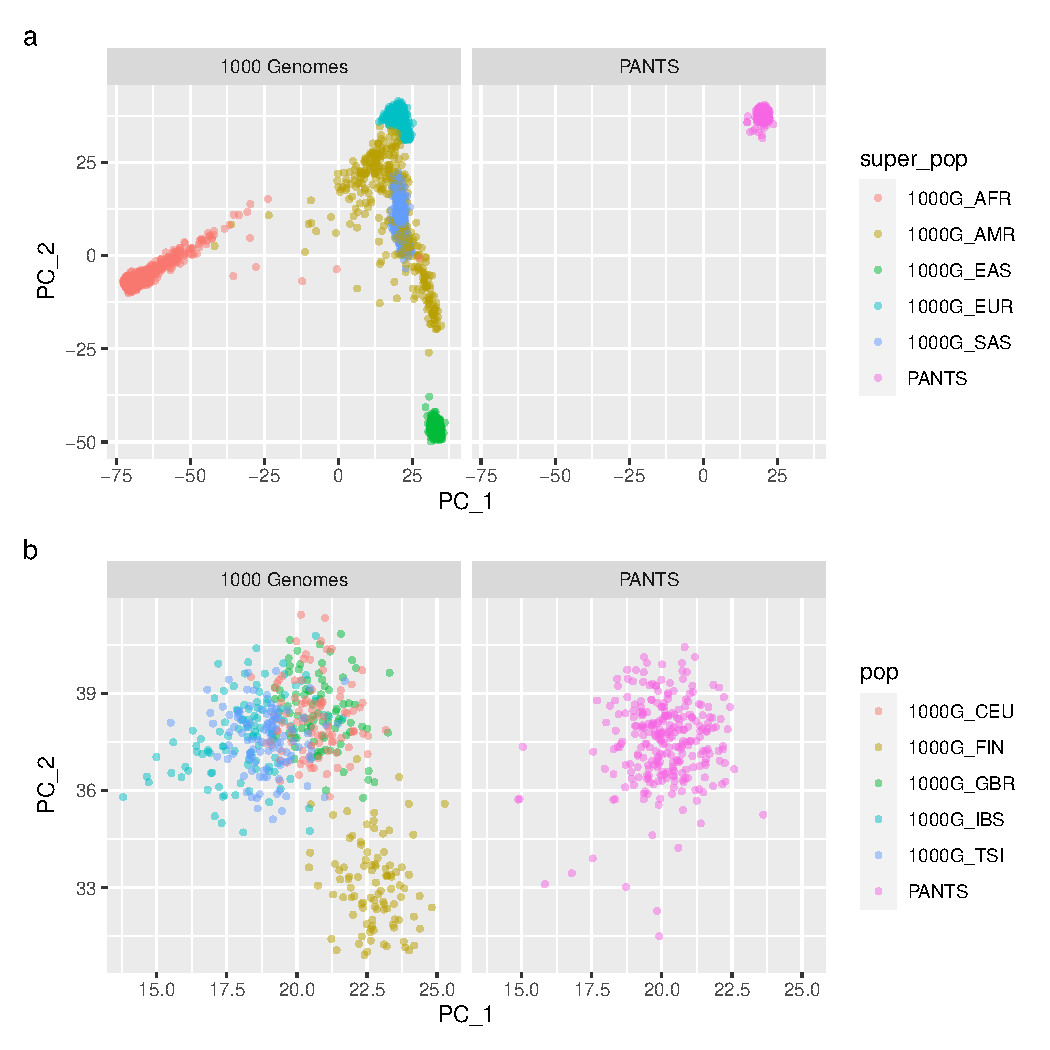
\includegraphics[width=1.0\textwidth,page=1]{mainmatter/figures/chapter_04/pants_samples.sampleids_cleaned_to_lowercase.filtered.GRCh38.sorted.multiPANTS.projection_1000G_pca.pdf}
    \caption{
        \textbf{1000G samples and PANTS samples projected onto 1000G genotype PC1 and PC2 axes, colored by superpopulation (a) and population (b).}
        1000G superpopulations: AFR = African, AMR = Ad Mixed American, EAS = East Asian, EUR = European, SAS = South Asian.
        1000G European populations: CEU = Utah Residents (CEPH) with Northern and Western European Ancestry, FIN = Finnish in Finland, GBR = British in England and Scotland, IBS = Iberian Population in Spain, TSI = Toscani in Italia.
    }
    \label{fig:multipants_genotype_akt_1000g_pca}
\end{figure}

\subsubsection{Finding hidden confounders in expression data}

Between-sample normalisation and variance stabilisation was applied to the counts matrix (DESeq2::vst), resulting in $\log_2$ scale expression estimates.
As described in \cref{sec:hird_reQTL_methods},
given known factors (response, drug, five scaled genotype \glspl{PC}, five cell proportions), 
{PEER} was used to find additional hidden factors that explain variance in the expression matrix for a large fraction of genes.
This is similar to the process undertaken in \cref{subsubsec:multiPANTS_var_selection}, but these hidden factors can be unmeasured.
To maximise efficiency for \textit{cis}-\gls{eQTL} mapping, 
the number of PEER factors retained for each timepoint was selected to maximise the number of genes with at least one significant \gls{eQTL} detected on chromosome 1 (\cref{fig:multipants_reqtl_PEER_k_choice}).
The selected numbers were 25, 20, 15, and 5 factors for weeks 0, 14, 30, and 54 respectively.

\begin{figure}
    \centering
    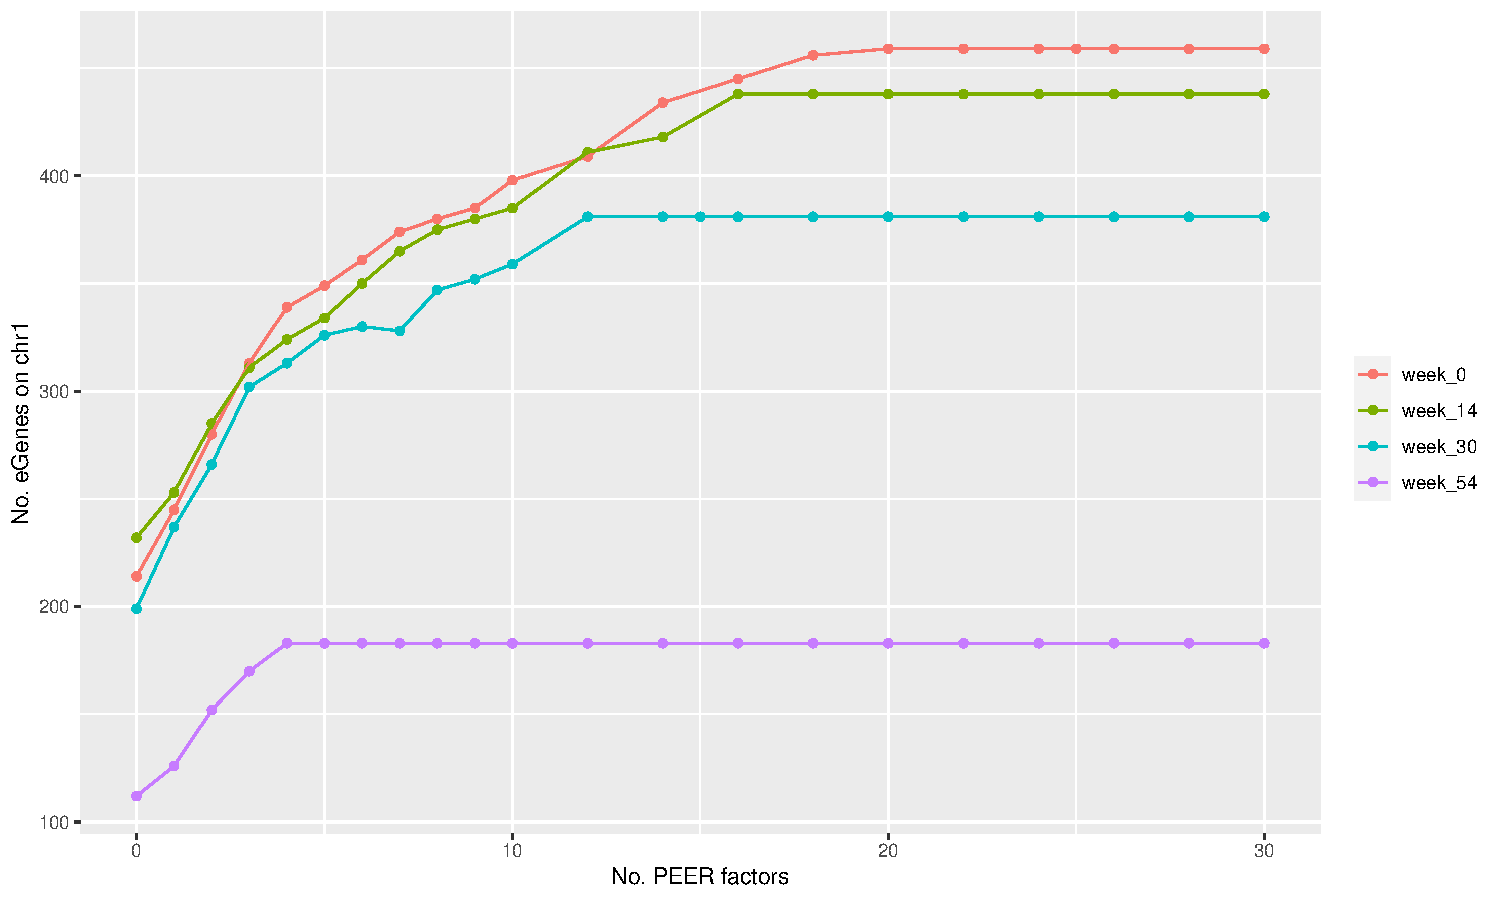
\includegraphics[width=1.0\textwidth,page=1]{mainmatter/figures/chapter_04/count_eGenes.signif_eGenes_vs_PEER_n.dataset_multiPANTS.chr_1.pdf}
    \caption{
        \textbf{Number of eGenes significant on chr1 vs. number of PEER factors included in \gls{eQTL} mapping as covariates.}
        \gls{FDR} computed with hierarchical Bonferroni-\gls{BH} \autocite{huang2018PowerFalseDiscovery} with significance threshold set at 0.05.
    }
    \label{fig:multipants_reqtl_PEER_k_choice}
\end{figure}

\subsubsection{Computing kinship matrices}

% NOTE: LDAK can account for genotype uncertainty, but Alex's data are rounded genotypes even for imputed variants.
\Gls{LOCO} kinship matrices were computed on typed \glspl{SNP} for each chromosome using LDAK as described in \cref{subsec:hird_reQTL_LDAK}.
% The kinship matrix will be incorporated into the \gls{eQTL} model to adjust for fine-scale population structure.

\subsubsection{Mapping \textit{cis}-\glsfmtshortpl{eQTL} in each timepoint separately}

As described in \cref{sec:hird_reQTL_methods},
\glspl{eQTL} were mapped in each timepoint using a linear mixed model in \software{limix}.
% Within each timepoint, patients with multiple samples (taken on different study days) had the non-major visit sample removed.
% although it may seem possible to have duplicate patients
%     following the stacking logic of TODO: cite,
%     it estimation of the alternative model log likelihood
%     excluding just a 2 duplicates at w14
%     makes LL alt much lower
%     LRT returns false negatives
%
%     resulting p value distribution is not well behaved:
%     large spike at 1
%
%     but the betas and stes remain comparable
%     since we use mashr to get signif values,
%     can keep these in or out.
% Although the \gls{eQTL} model form does not prohibit duplicate samples,
% it led to strange behaviour in limix where \gls{eQTL} betas and standard errors were comparable to the dedeuplicated results,
% but log-likelihood estimates were abnormally high.
% The deduplicated sample sizes at weeks 0, 14, 30 and 54 were 223, 205, 167, and 84.
The sample sizes with both genotype and expression data available for \gls{eQTL} mapping at weeks 0, 14, 30 and 54 were 223, 205, 167, and 84 respectively.

% TODO:
% The number of genes was 15592, which is more than in the DGE. Probably different filtering pipeline versions...
% OR is it 15040?
%
% The Ensembl gene start and end coordinates correspond to the outermost transcript start and end coordinates.
For each autosomal gene, \textit{cis}-\glspl{SNP} within 1 Mb of the Ensembl gene start (gene end on the minus strand),
were filtered to keep \glspl{SNP} where the number of samples homozygous for the minor allele was at least 5.
Small group numbers lead to data points with high leverage that may be unduly influential on the genotype beta.
% This is done in place of a per-timepoint \gls{MAF} or minor allele count filters.
Assuming \gls{HWE}, this is equivalent to a \gls{MAF} filter of 
$\sqrt{5/(223\times2)} = \num{0.1058809}$ in the timepoint with the largest sample size (week 0),
and $\sqrt{5/(84\times2)} = \num{0.1725164}$ in the timepoint with the smallest sample size (week 54).

The limix model for each \gls{SNP}-gene pair had 
$\log_2$ expression as the response variable
and genotype dosage as the predictor of interest.
Other fixed effect predictors were
the intercept,
known factors (response, drug, five scaled genotype \glspl{PC}, cell proportions), 
and PEER hidden factors (timepoint-specific number selected above).
A random intercept term was also included with mean zero and covariance matrix proportional to the \gls{LOCO} kinship matrix for the \gls{SNP}'s chromosome.

\subsubsection{Joint \glsfmtshortpl{reQTL} mapping over all timepoints}

As described in \cref{sec:hird_reQTL_methods},
summary statistics from per-timepoint mapping were input to \software{mashr} \autocite{urbut2018FlexibleStatisticalMethods} to map \gls{eQTL} jointly over all timepoints.
A total of \num{25908527} \glspl{SNP} were tested in all timepoints.
% TODO useEstimateNullCorrelationSimple_TRUE
The null correlation structure of the timepoints was estimated using null tests within a random subset of \num{200000} tests.
Data-driven covariance matrices representing patterns of effects across timepoints were estimated using a strong subset of tests.
As the strong subset should contain \gls{eQTL} that are likely to have an effect in at least one timepoint,
for each gene and timepoint, I selected the \gls{eQTL} with the smallest \pvalue{}, if that \pvalue{} was < 0.05, resulting in a strong subset of \num{129002} tests.
The mash model was fit on the full random subset, accounting for the computed null correlation and covariance matrices, in exchangeable Z-scores mode.
Finally, posterior betas and standard errors were computed for all tests using the fitted model parameters.
A corresponding \gls{lfsr} is also returned, controlling for multiple testing.
% TODO describe mashr bug for negative betas being capped for lfsr

The lead \gls{eQTL} for each gene was chosen as the \gls{eQTL} with the lowest \gls{lfsr} in any condition, 
breaking ties by highest INFO, highest \gls{MAF}, shortest dist to gene start (or end), and smallest genomic coordinate.
Each lead \gls{eQTL} was assessed for being a significant \gls{reQTL} by a Z test for whether the difference in betas was zero, between the week 0 beta and each of the other three weeks.
Multiple testing for the number of genes was controlled using the \gls{BH} \gls{FDR} for each of the three comparisons separately.

% \subsubsection{Clustering reQTLs}

% \1 <pipeline>
%     \2 align
%     \2 Centering, no scaling
%         \3 ensure comparability between gene
%         \3 Amplifies noise? Migitate by prefiltering on nominal signif diff between two timepoints
%     https://hdbscan.readthedocs.io/en/latest/comparing_clustering_algorithms.html
%     \2 dist\_cor(method='pearson')
%     \2 fastcluster::hclust(method='complete')
%     \2 distance metric 1-cor(pearson)
%     •	https://www.rdocumentation.org/packages/NbClust/versions/3.0/topics/NbClust
%     o	Possible statistics: the index to be calculated. This should be one of : "kl", "ch", "hartigan", "ccc", "scott", "marriot", "trcovw", "tracew", "friedman", "rubin", "cindex", "db", "silhouette", "duda", "pseudot2", "beale", "ratkowsky", "ball", "ptbiserial", "gap", "frey", "mcclain", "gamma", "gplus", "tau", "dunn", "hubert", "sdindex", "dindex", "sdbw", "all" (all indices except GAP, Gamma, Gplus and Tau), "alllong" (all indices with Gap, Gamma, Gplus and Tau included).
%     \2 Number of clusters: gap stat fviz\_nbclust

\section{Results}
% \todo{what to put in results vs discussion. going with the pattern of providing enough info for the reader to intepret the data in the results, then doing a summary and my own interpretation in the discussion}

\subsection{Longitudinal \glsfmtshort{RNAseq} data from the \glsfmtshort{PANTS} cohort}

To define transcriptomic differences between primary responders and non-responders to anti-\gls{TNF} therapy in the \gls{PANTS} cohort, 
I analysed whole blood \gls{RNAseq} gene expression measured at up to four timepoints per patient:
week 0 baseline before commencing anti-\gls{TNF} therapy, and weeks 14, 30 and 54 after commencing anti-\gls{TNF} therapy.
% \todo{Some primary non-responders have loss of response samples. Not sure why.}
After quality control, expression data was available for 15584 genes and 814 samples.
These samples come from 324 patients, whose characteristics are shown in \cref{tab:multipants_table1}.
The proportion of primary non-responders is high (43.8\%) compared to the overall proportion in the \gls{PANTS} cohort (23.8\%, \autocite{kennedy2019PredictorsAntiTNFTreatment}).
This is due to sample selection for \gls{RNAseq} to balance the sample size for each combination of drug and primary response status.

% Table 1. 
% latex table generated in R 3.6.2 by xtable 1.8-4 package
% Fri Sep  4 19:08:12 2020
\begin{table}[]
\centering
\caption[\captionshort{Patient characteristics for the \gls{PANTS} \gls{RNAseq} subcohort.}]{\textbf{Patient characteristics for the \gls{PANTS} \gls{RNAseq} subcohort.} Values are count and percentage for categorical variables; mean and standard deviation for continuous variables; \pvalues{} are for the comparison between drugs.}\label{tab:multipants_table1}
\begin{adjustbox}{width=0.9\textwidth,height=0.9\textheight,keepaspectratio}
\begin{tabular}{lrrrr}
  \hline
  & adalimumab (ADA) & infliximab (IFX) & drugs pooled & p-value \\ 
  \hline
\textbf{Sex      } &  &  &  & 0.317 \\ 
  \hskip .5cm   (Col \%) &  &  &  & Fisher exact \\ 
  \hskip .5cm   FEMALE & 78 (48.4\%) & 89 (54.6\%) & 167 (51.5\%) &  \\ 
  \hskip .5cm   MALE & 83 (51.6\%) & 74 (45.4\%) & 157 (48.5\%) &  \\ 
    \textbf{Age of onset (years)      } &  &  &  & 0.774 \\ 
  \hskip .5cm    Mean (SD) & 33.3 (15.4) & 32.8 (15.3) & 33.1 (15.3) & Wilcoxon rank-sum \\ 
  \hskip .5cm    Missing & 0 & 0 & 0 &  \\ 
    \textbf{Disease duration (years)      } &  &  &  & 0.546 \\ 
  \hskip .5cm    Mean (SD) & 6.1 (8.1) & 5.9 (7.7) & 6.0 (7.9) & Wilcoxon rank-sum \\ 
  \hskip .5cm    Missing & 0 & 0 & 0 &  \\ 
    \textbf{Smoking status      } &  &  &  & 0.263 \\ 
  \hskip .5cm   (Col \%) &  &  &  & Fisher exact \\ 
  \hskip .5cm   Current & 28 (17.4\%) & 36 (22.1\%) & 64 (19.8\%) &  \\ 
  \hskip .5cm   Ex & 55 (34.2\%) & 43 (26.4\%) & 98 (30.2\%) &  \\ 
  \hskip .5cm   Never & 78 (48.4\%) & 84 (51.5\%) & 162 (50.0\%) &  \\ 
    \textbf{Crohn's-related surgery      } &  &  &  & 0.549 \\ 
  \hskip .5cm   (Col \%) &  &  &  & Fisher exact \\ 
  \hskip .5cm   FALSE & 114 (70.8\%) & 110 (67.5\%) & 224 (69.1\%) &  \\ 
  \hskip .5cm   TRUE & 47 (29.2\%) & 53 (32.5\%) & 100 (30.9\%) &  \\ 
    \textbf{On immunomodulator ever      } &  &  &  & 0.543 \\ 
  \hskip .5cm   (Col \%) &  &  &  & Fisher exact \\ 
  \hskip .5cm   FALSE & 23 (14.3\%) & 28 (17.2\%) & 51 (15.7\%) &  \\ 
  \hskip .5cm   TRUE & 138 (85.7\%) & 135 (82.8\%) & 273 (84.3\%) &  \\ 
    \textbf{On immunomodulator at baseline      } &  &  &  & 0.912 \\ 
  \hskip .5cm   (Col \%) &  &  &  & Fisher exact \\ 
  \hskip .5cm   FALSE & 79 (49.1\%) & 81 (49.7\%) & 160 (49.4\%) &  \\ 
  \hskip .5cm   TRUE & 82 (50.9\%) & 82 (50.3\%) & 164 (50.6\%) &  \\ 
    \textbf{On corticosteroids at baseline      } &  &  &  & 0.011 \\ 
  \hskip .5cm   (Col \%) &  &  &  & Fisher exact \\ 
  \hskip .5cm   FALSE & 113 (70.2\%) & 92 (56.4\%) & 205 (63.3\%) &  \\ 
  \hskip .5cm   TRUE & 48 (29.8\%) & 71 (43.6\%) & 119 (36.7\%) &  \\ 
    \textbf{Baseline BMI      } &  &  &  & 0.237 \\ 
  \hskip .5cm    Mean (SD) & 25.2 (6.2) & 24.3 (5.5) & 24.8 (5.9) & Wilcoxon rank-sum \\ 
  \hskip .5cm    Missing & 0 & 0 & 0 &  \\ 
    \textbf{Primary response status      } &  &  &  & 0.263 \\ 
  \hskip .5cm   (Col \%) &  &  &  & Fisher exact \\ 
  \hskip .5cm   Primary non-response & 76 (47.2\%) & 66 (40.5\%) & 142 (43.8\%) &  \\ 
  \hskip .5cm   Primary response & 85 (52.8\%) & 97 (59.5\%) & 182 (56.2\%) &  \\ 
    \textbf{CD8+ T cell (\%)      } &  &  &  & 0.380 \\ 
  \hskip .5cm    Mean (SD) & 2.8 (4.2) & 2.8 (5.2) & 2.8 (4.7) & Wilcoxon rank-sum \\ 
  \hskip .5cm    Missing & 38 & 18 & 56 &  \\ 
    \textbf{CD4+ T cell (\%s)      } &  &  &  & 0.752 \\ 
  \hskip .5cm    Mean (SD) & 9.2 (6.3) & 9.2 (6.8) & 9.2 (6.5) & Wilcoxon rank-sum \\ 
  \hskip .5cm    Missing & 38 & 18 & 56 &  \\ 
    \textbf{B cell (\%s)      } &  &  &  & 0.094 \\ 
  \hskip .5cm    Mean (SD) & 1.9 (2.0) & 1.5 (1.9) & 1.7 (1.9) & Wilcoxon rank-sum \\ 
  \hskip .5cm    Missing & 38 & 18 & 56 &  \\ 
    \textbf{Monocyte (\%s)      } &  &  &  & 0.497 \\ 
  \hskip .5cm    Mean (SD) & 8.9 (3.5) & 9.2 (3.7) & 9.0 (3.6) & Wilcoxon rank-sum \\ 
  \hskip .5cm    Missing & 38 & 18 & 56 &  \\ 
    \textbf{NK cell (\%s)      } &  &  &  & 0.683 \\ 
  \hskip .5cm    Mean (SD) & 1.9 (3.2) & 1.9 (3.8) & 1.9 (3.5) & Wilcoxon rank-sum \\ 
  \hskip .5cm    Missing & 38 & 18 & 56 &  \\ 
    \textbf{Granulocyte (\%s)      } &  &  &  & 0.911 \\ 
  \hskip .5cm    Mean (SD) & 74.3 ( 9.7) & 74.3 (10.8) & 74.3 (10.3) & Wilcoxon rank-sum \\ 
  \hskip .5cm    Missing & 38 & 18 & 56 &  \\ 
     \hline
\end{tabular}
\end{adjustbox}
\end{table}



\subsection{Baseline gene expression associated with primary response}

% TODO: increased expression vs upreg: make this all consistent
% TODO: after primary response mentioned, just drop primary 

Patient primary response to anti-\gls{TNF} was defined at week \numrange{12}{14} (after the induction period) according to the clinical decision algorithm from \textcite{kennedy2019PredictorsAntiTNFTreatment} described in \cref{multiPANTS:PR_definition}, 
which integrates clinician assessment with change in \gls{CRP} level and \gls{HBI} score.
To identify differences in baseline gene expression associated with future primary response, 
I fit per-gene linear models at 15511 genes, comparing week 0 gene expression in primary responders with primary non-responders.
Comparisons were performed both within infliximab-only and adalimumab-only subgroups, and with both drugs pooled.
Models were run both adjusting for cell composition estimates of six immune cell types, and without adjustment.
% TODO: make FDR= after this all consistent formatting
Throughout this section, the significance threshold was set at $\text{\gls{FDR}} < 0.05$ for each comparison, and positive $\log_2\text{\glspl{FC}}$ indicate increased expression in responders versus non-responders.

Without adjusting for cell composition, the largest effects were infliximab-only, with 859 genes differentially expressed.
Only \gene{KCNN3} ($\log_2\text{\gls{FC}}=\num{-0.843455423}$) was significant for the adalimumab-only comparison, 
% logFC      AveExpr         t      P.Value   adj.P.Val     z.std
% 0.34597454 6.55605 4.9264804 1.094745e-06 0.016980595 4.8737951
% 0.31379161 6.55605 4.6913403 3.384743e-06 0.050291627 4.6459748
and only \gene{SIGLEC10} ($\log_2\text{\gls{FC}} = \num{0.34597454}$) was significant in the pooled analysis (\cref{fig:multipants_dge_volcano_week_0_R_N}).

After adjustment for cell composition, there were no longer any significant genes in the infliximab-only analysis, 
with 856/859 genes that were significant before the comparison having a dampened effect size after correction (smaller absolute effect and same sign), suggesting many effects may be mediated by cell composition.
\gene{SIGLEC10} in the combined analysis was also non-significant after adjustment (adjusted $\log_2\text{\gls{FC}} = \num{0.31379161}$, FDR=\num{0.050291627}).
Conversely, at three genes downregulated in the adalimumab-only analysis that were the only significant genes post-adjustment, I observed increased significance:
%       logFC  AveExpr          t      P.Value  adj.P.Val      z.std
% -0.33495771 2.569096 -4.5040835 7.723531e-06 0.05989985 -4.4727077
% -0.35115926 2.569096 -5.0627658 5.212334e-07 0.00677703 -5.0183272
\gene{PDIA5} (unadjusted $\log_2\text{\gls{FC}} = \num{-0.33495771}$, adjusted $\log_2\text{\gls{FC}} = \num{-0.35115926}$), 
% -0.843455423 -0.2360221 -4.7304059 2.689467e-06 0.04171633 -4.69321336
% -0.879776701 -0.2360221 -4.9610155 8.738353e-07 0.00677703 -4.91811062
\gene{KCNN3} (\num{-0.843455423}, \num{-0.879776701}), 
% -1.1529588 1.169468 -4.212961 2.854891e-05 0.1476074 -4.184743
% -1.2231591 1.169468 -4.479679 8.738258e-06 0.0451797 -4.446249
and \gene{IGKV1-9} (\num{-1.1529588}, \num{-1.2231591}).

To identify coordinately up and downregulated gene sets and increase sensitivity for detecting differences between responders and non-responders,
I performed rank-based gene set analysis in on the per-gene $z$-statistics using blood transcriptomic modules: annotated sets of coexpressed genes in peripheral whole blood from \textcite{li2013MolecularSignaturesAntibody} (prefixed \enquote{LI}).
This module-level analysis was also run unadjusted (\cref{fig:multipants_dge_panelPlot_week_0_R_N_cellPropF}) and adjusted for cell composition (\cref{fig:multipants_dge_panelPlot_week_0_R_N_cellPropT}).

Despite only \gene{SAMD10} having a significantly different effect between drugs at the gene-level (a significant interaction between drug and response at week 0), 
the large global differences observable in \cref{fig:multipants_dge_volcano_week_0_R_N} were detected in the module-level analysis\footnote{
It is likely the study is not powered to detect gene-level three-way interaction effects between timepoint, drug and response.
I am not aware of which subgroup analyses may have been prespecified during the study design and sample size calculations for the \gls{PANTS} \gls{RNAseq} cohort.
}.
Without adjusting for cell composition, many of the most significantly upregulated modules in the pooled analysis, 
including upregulation of monocyte (LI.M11.0, LI.S4), neutrophil (LI.M37.1, LI.M11.2), and dendritic cell (LI.M165, LI.S11),
appear to be driven an infliximab-specific effect.
These modules have heavily reduced significance after adjusting for cell composition.
The new modules that are most upregulated in the pooled analysis after adjustment have more consistent effects between drugs, such as
MHC-TLR7-TLR8 cluster (LI.M146), antigen presentation (LI.M71, LI.M95.0), and myeloid cell enriched receptors and transporters (LI.M4.3).

For downregulated modules before adjustment, I observed infliximab-specific effects for NK cell (LI.M7.2) and T cell (LI.M7.0, LI.M7.1) modules.
Adalimumab-specific effects were observed for plasma cell, B cell and immunoglobulin modules (LI.M156.0, LI.M156.0, LI.S3); and cell cycle and transcription modules (LI.M4.0, LI.M4.1).
After adjustment, the significance of infliximab-specific modules was reduced, 
but the significance of adalimumab-specific modules and the corresponding interaction effects was increased.
% \todo{Carl's comment here: What happens to the significance of cell-type specific gene-sets when you condition on that cell-type. Do they uniformly decrease? Do you think this could mean that these signals (and others) are driven by differences in cell composition, but that you have cell composition imperfectly estimated and thus are not fully correcting for variance in cell composition?}
In both gene-level and module-level results, where comparing baseline expression between responders and non-responders, there is a striking heterogeneity between patients on infliximab and adalimumab that is only partially reduced by cell proportion adjustment.

\begin{figure}
    \centering
    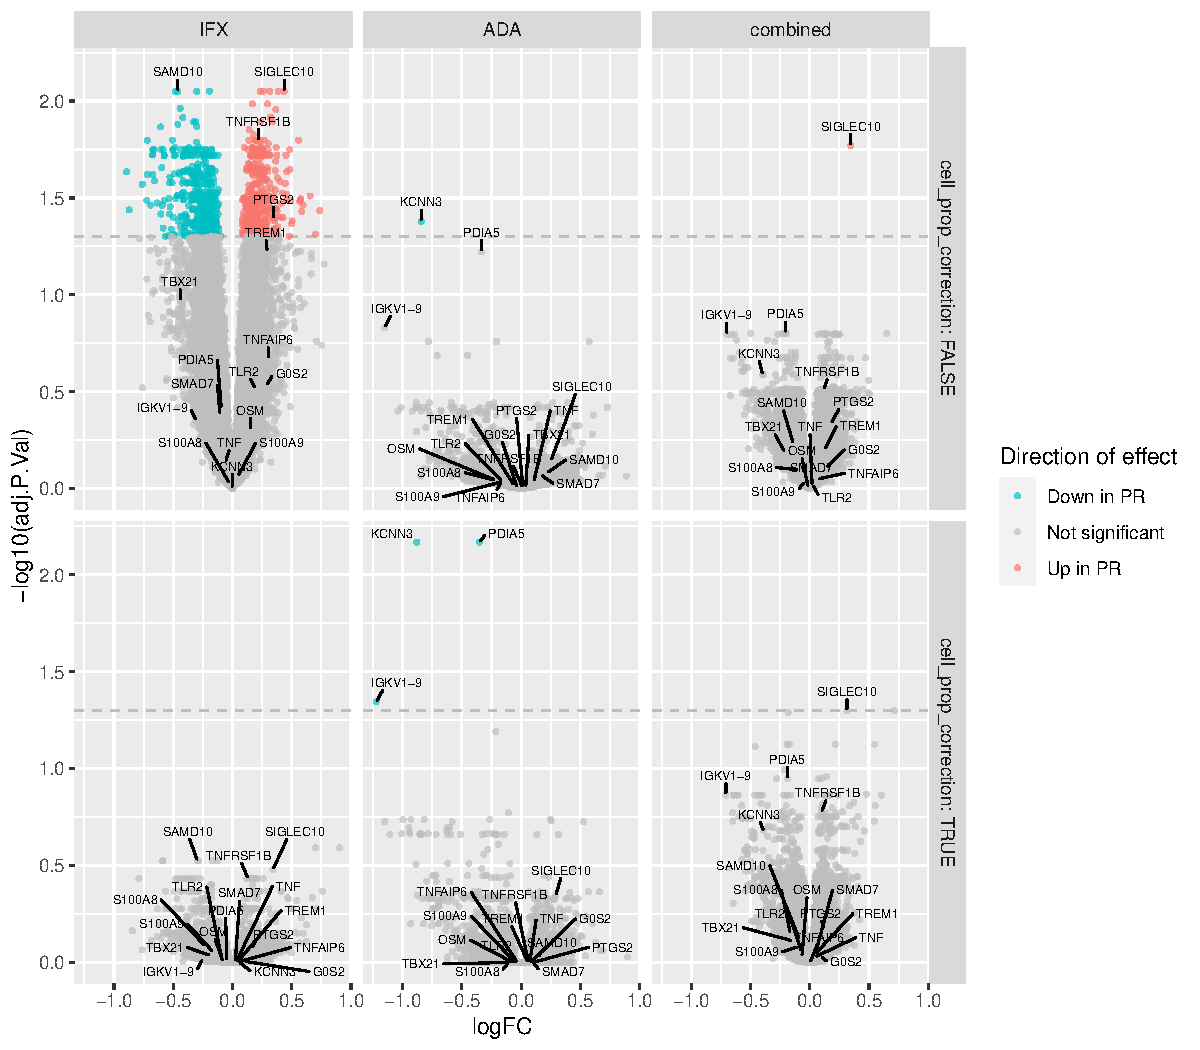
\includegraphics[width=1.0\textwidth,page=1]{mainmatter/figures/chapter_04/plot_gene_set_enrichment.dge_result_volcano_simple_C_1RI_1NI,C_1RA_1NA,C_1R_1N.pdf}
    \caption{
        \textbf{Volcano plots of \gls{DGE} between primary responders and non-responders at week 0; unadjusted (top row) and adjusted (bottom row) for cell composition; for infliximab (IFX), adalimumab (ADA), or with both drugs pooled.}
        Annotated genes include significant associations from this study and previously reported associations from \autoref{subsec:multiPANTS_intro_predicting_response}.
        Dashed line shows significance threshold at FDR = 0.05.
        PR = primary responder.
    }
    \label{fig:multipants_dge_volcano_week_0_R_N}
\end{figure}

% \begin{figure}
%     \centering
%     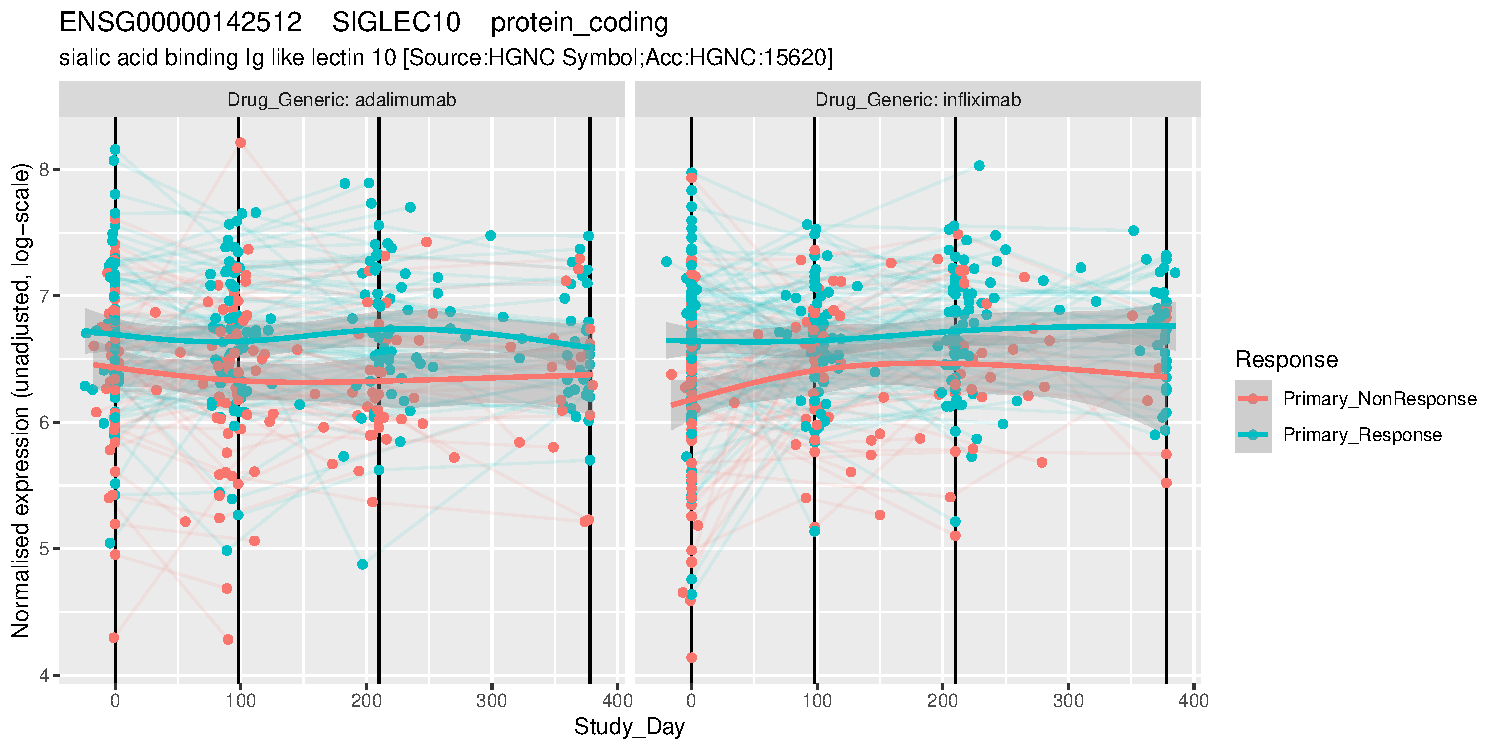
\includegraphics[width=1.0\textwidth,page=1]{mainmatter/figures/chapter_04/dream.E_vs_Study_Day.GENEID_ENSG00000142512.SYMBOL_SIGLEC10.pdf}
%     \caption{Unadjusted, normalised SIGLEC10 expression over time}
%     \label{fig:multipants_dge_SIGLEC10}
% \end{figure}

\begin{figure}
    \centering
    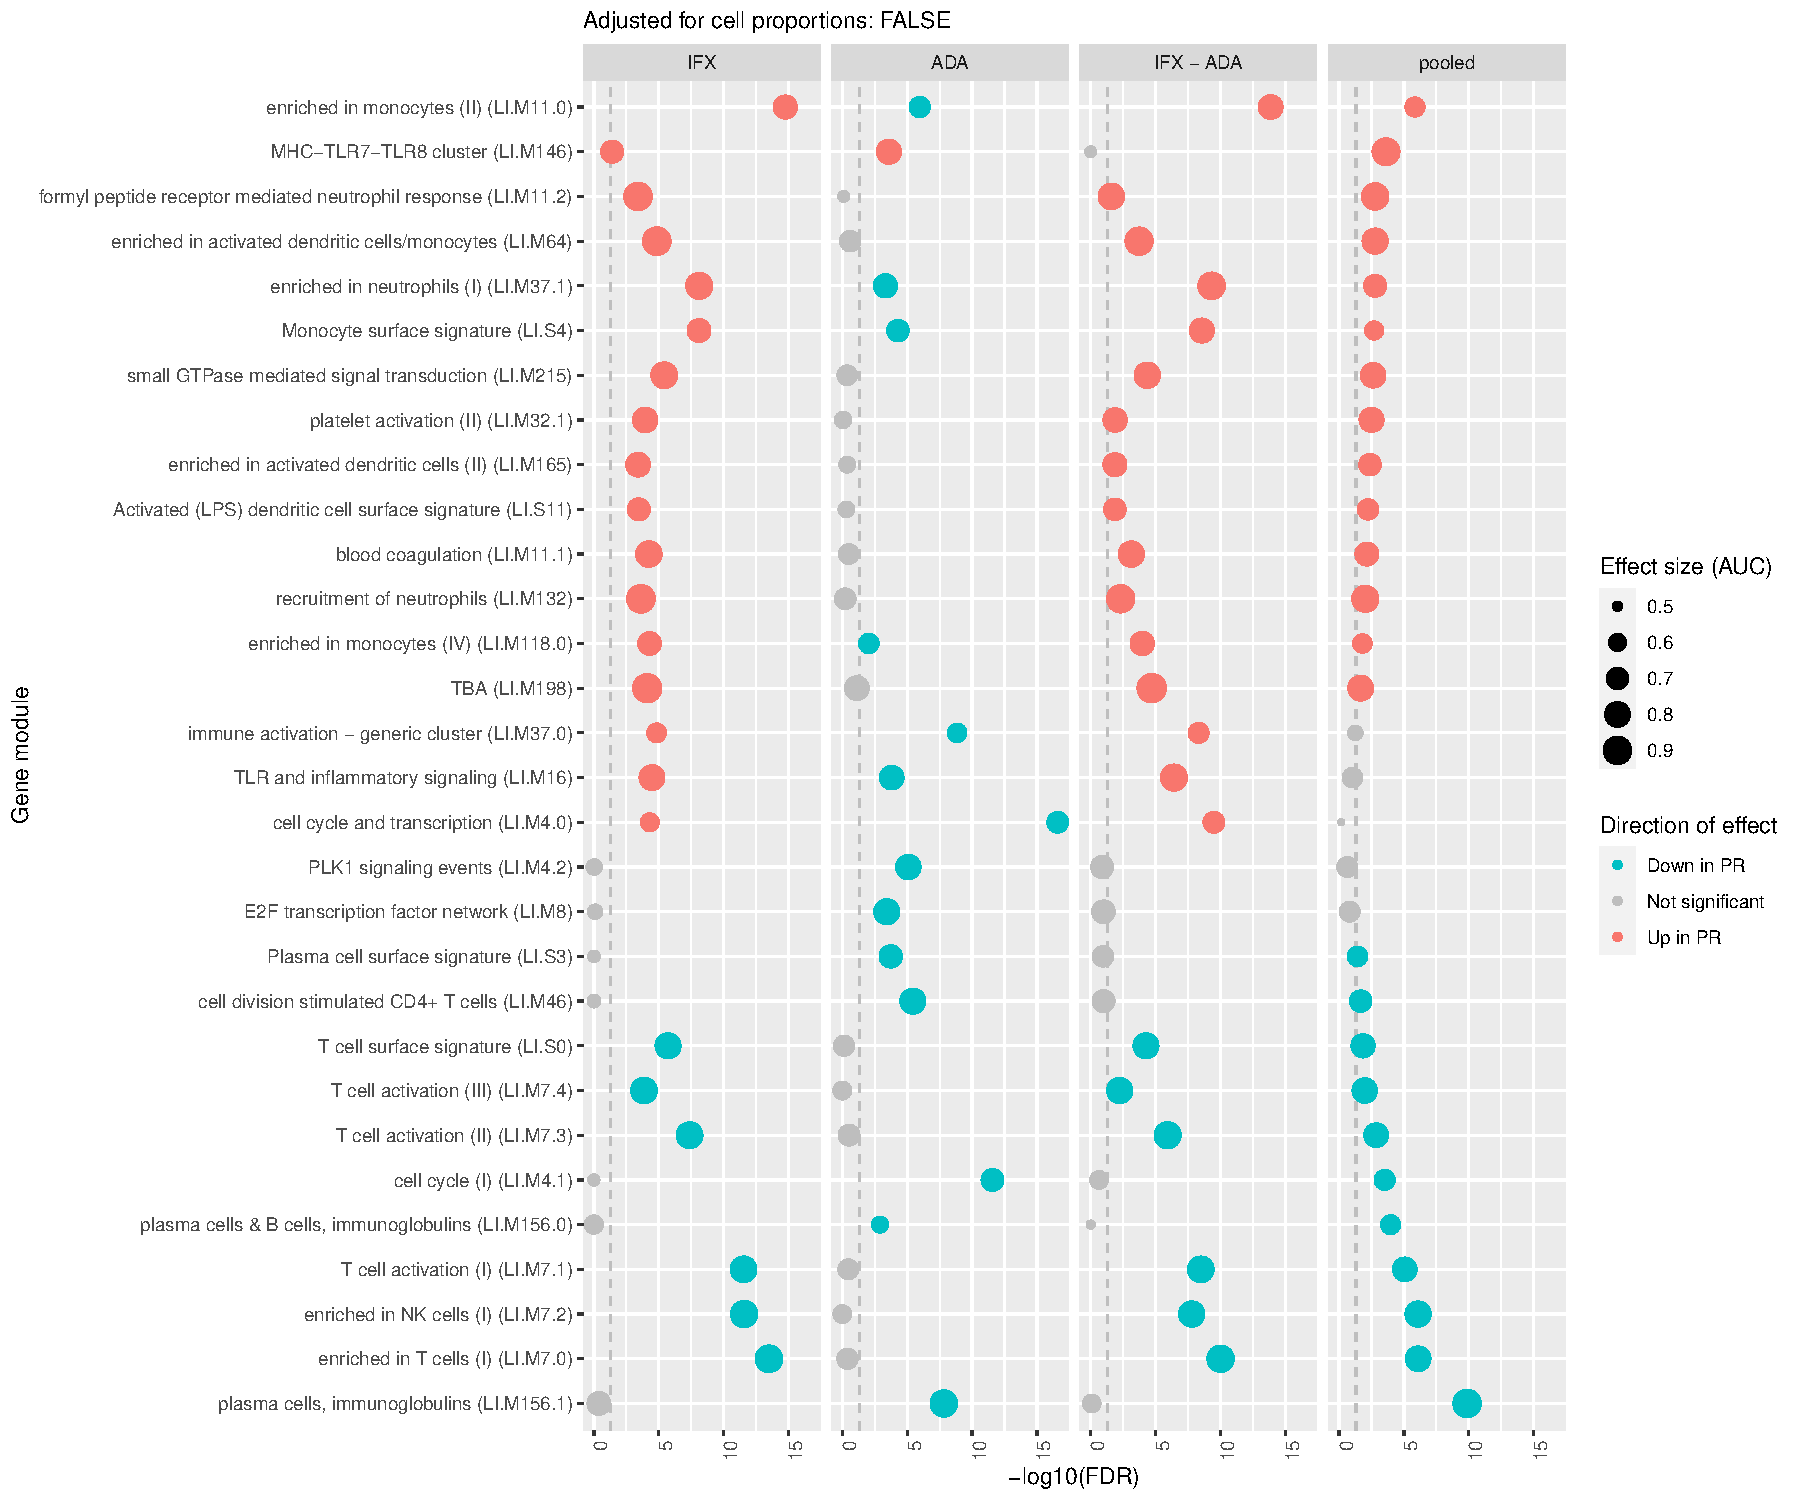
\includegraphics[width=1.0\textwidth,page=1]{mainmatter/figures/chapter_04/plot_gene_set_enrichment.tmodCERNO_panelplot_reversed_C_1RI_1NI,C_1RA_1NA,C_(1RI_1NI)_(1RA_1NA),C_1R_1N.cell_prop_correction_FALSE.pdf}
    \caption{
        \textbf{Top modules differentially expressed between primary responders and non-responders at week 0, unadjusted for cell composition.}
        Columns correspond to results from infliximab (IFX), adalimumab (ADA), infliximab-adalimumab difference and pooled analyses. 
        The top 30 modules ranked by minimum \gls{FDR} in any column are shown. Vertical dashed line shows significance threshold at FDR = 0.05.
        PR = primary responder.
    }
    \label{fig:multipants_dge_panelPlot_week_0_R_N_cellPropF}
\end{figure}

\begin{figure}
    \centering
    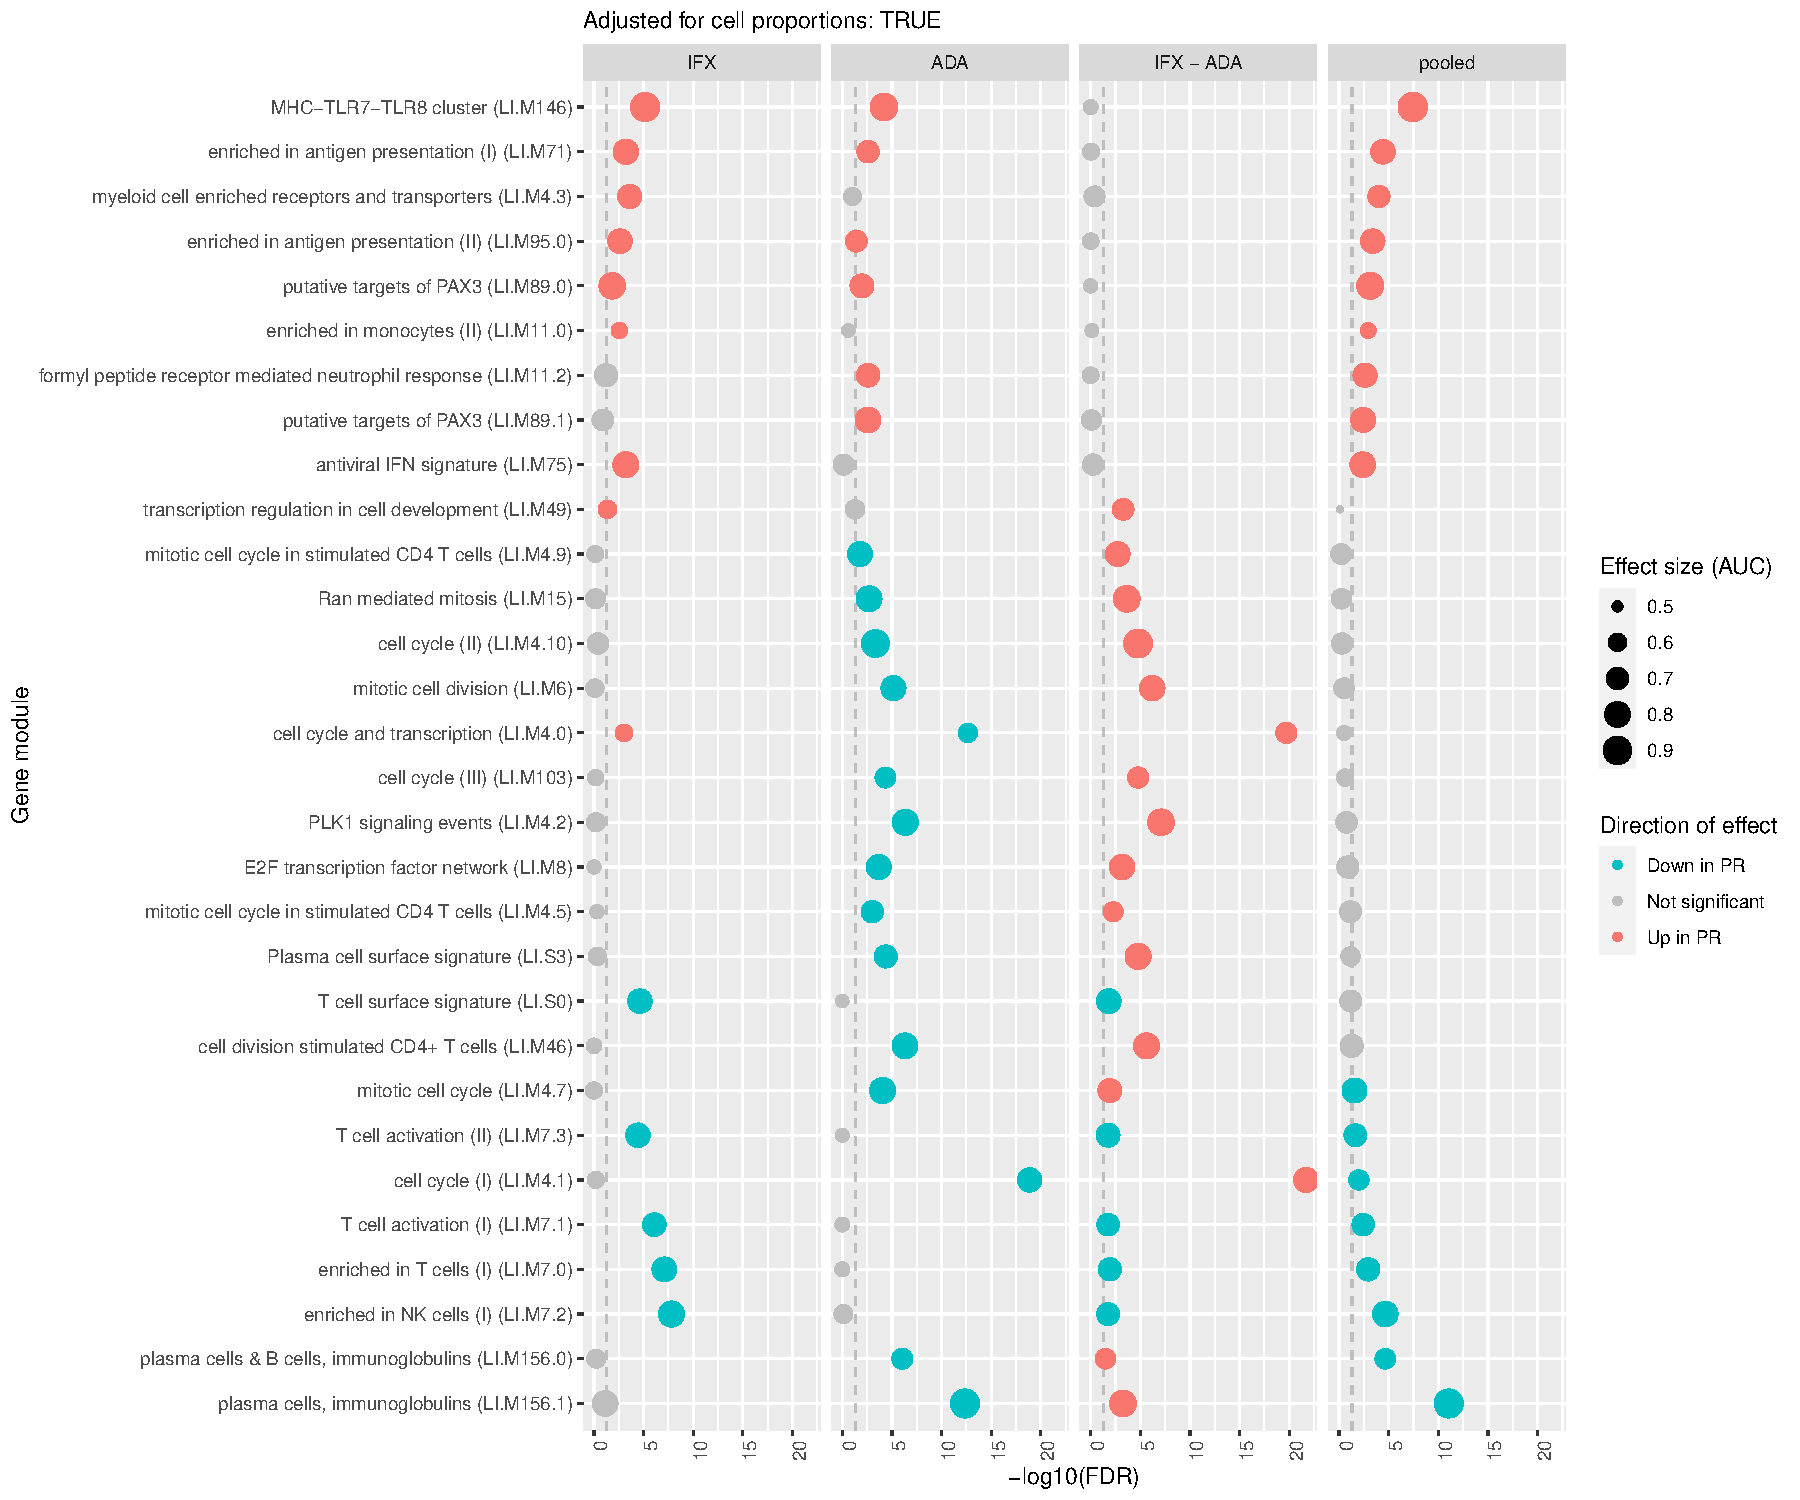
\includegraphics[width=1.0\textwidth,page=1]{mainmatter/figures/chapter_04/plot_gene_set_enrichment.tmodCERNO_panelplot_reversed_C_1RI_1NI,C_1RA_1NA,C_(1RI_1NI)_(1RA_1NA),C_1R_1N.cell_prop_correction_TRUE.pdf}
    \caption{
        \textbf{Top modules differentially expressed between primary responders and non-responders at week 0, adjusted for cell composition.}
        Columns correspond to results from infliximab (IFX), adalimumab (ADA), infliximab-adalimumab difference and pooled analyses. 
        The top 30 modules ranked by minimum \gls{FDR} in any column are shown. Vertical dashed line shows significance threshold at FDR = 0.05.
        PR = primary responder.
    }
    \label{fig:multipants_dge_panelPlot_week_0_R_N_cellPropT}
\end{figure}

\subsection{Assessing previously reported baseline predictors of primary response}

% genes_to_label_list <- list(
%     c(
%         'SIGLEC10', 'PDIA5', 'KCNN3', 'IGKV1-9', 'SAMD10',
%         # Verstockt 2019
%         'TREM1', 'OSM', 'TNF', 'TNFRSF1B', 'IL13RA2',
%         # arijs2009MucosalGeneSignatures
%         'TNFRSF11B', 'STC1', 'PTGS2', 'IL13RA2', 'IL11',
%         # Arijs 2010 \url{https://academic.oup.com/ibdjournal/article/16/12/2090/4628294}
%         'TNFAIP6', 'S100A8', 'G0S2', 'S100A9', 'IL11',
%         # salvador-martin2020GeneSignaturesEarly
%         'SMAD7', 'TLR2', 'DEFA5', 'TBX21'
%         # 'CD14', 'FCGR1A', 'CCR1', 'SELL', # c from https://www.ncbi.nlm.nih.gov/pmc/articles/PMC2804287/
%         # 'FCGR3A', 'PECAM1', 'CX3CR1', 'ITGAL' # nc from https://www.ncbi.nlm.nih.gov/pmc/articles/PMC2804287/
%         # 'LAIR2' 'ASAH1', 'APOBEC3A', 'TSPAN14', 'LIPA' # mono2 from https://science.sciencemag.org/content/356/6335/eaah4573
%     ),
%     c(
%         'SIGLEC10', 'PDIA5', 'KCNN3', 'IGKV1-9', 'SAMD10',
%         # Verstockt 2019
%         'TREM1', 'OSM', 'TNF', 'TNFRSF1B', 'IL13RA2',
%         # arijs2009MucosalGeneSignatures
%         'TNFRSF11B', 'STC1', 'PTGS2', 'IL13RA2', 'IL11',
%         # Arijs 2010 \url{https://academic.oup.com/ibdjournal/article/16/12/2090/4628294}
%         'TNFAIP6', 'S100A8', 'G0S2', 'S100A9', 'IL11',
%         # salvador-martin2020GeneSignaturesEarly
%         'SMAD7', 'TLR2', 'DEFA5', 'TBX21'
%         # 'CD14', 'FCGR1A', 'CCR1', 'SELL', # c from https://www.ncbi.nlm.nih.gov/pmc/articles/PMC2804287/
%         # 'FCGR3A', 'PECAM1', 'CX3CR1', 'ITGAL' # nc from https://www.ncbi.nlm.nih.gov/pmc/articles/PMC2804287/
%         # 'LAIR2' 'ASAH1', 'APOBEC3A', 'TSPAN14', 'LIPA' # mono2 from https://science.sciencemag.org/content/356/6335/eaah4573
%     )
% )
In addition to hits from this study, \cref{fig:multipants_dge_volcano_week_0_R_N} is annotated with genes whose expression in gut biopsies or blood has been previously evaluated for baseline prediction of primary response \autocite{arijs2009MucosalGeneSignatures,arijs2010PredictiveValueEpithelial,verstockt2019LowTREM1Expression,salvador-martin2020GeneSignaturesEarly}.
Some genes expressed in gut mucosa (e.g. \gene{IL13RA2}) were not appreciably expressed in this whole blood dataset, 
and most other genes that were expressed were not significantly differentially expressed.
Only \gene{TNFRSF1B} and \gene{PTGS2} were associated with primary response, upregulated in at baseline in responders, specifically in the infliximab-only comparison, unadjusted for cell composition.
\gene{TNFRSF1B} was found by \textcite{verstockt2019LowTREM1Expression} to be downregulated in baseline inflamed mucosal biopsies of responders to anti-\gls{TNF} therapy in \gls{IBD} patients (n=44, FC=0.72, p=.008).
\gene{PTGS2} was found by \textcite{arijs2009MucosalGeneSignatures} to be downregulated in baseline mucosal biopsies of responders to infliximab for Crohn's colitis (n=46).
The directions of effect in both cases are opposite to this study, but comparisons are hard to draw between blood and mucosal biopsies.

A previously identified marker in blood, \gene{TREM1} was found to have opposing effects in two studies by \textcite{gaujoux2019CellcentredMetaanalysisReveals} (n=22) and \textcite{verstockt2019LowTREM1Expression} (n=54).
\gene{TREM1} had the strongest differences between responders and non-responders at baseline in infliximab subcohort, 
but did not reach significance before ($\log_2\text{\gls{FC}} = \num{0.29283535}$, FDR=\num{0.0595323})
%      logFC  AveExpr          t    P.Value adj.P.Val      z.std
% 0.29283535 7.668094  2.8665957 0.00429233 0.0595323  2.8558388
nor after adjusting for cell composition ($\log_2\text{\gls{FC}} = \num{0.04625626}$, FDR=\num{0.9864125}).
% 0.04625626 7.668094  0.6661333 0.50560221 0.9864125  0.6657010
The combined sample size in this study for the infliximab subcohort at baseline was is n=145 (\cref{fig:multipants_studyDay_boxplots}), so it is expected the power in this study is greater.

% TODO: confint not implemented in variancePartition for topTable on dream objects, and multiplicity adjustment is non-trivial, see \url{https://amstat.tandfonline.com/doi/abs/10.1198/016214504000001907}

% \begin{figure}
%     \centering
%     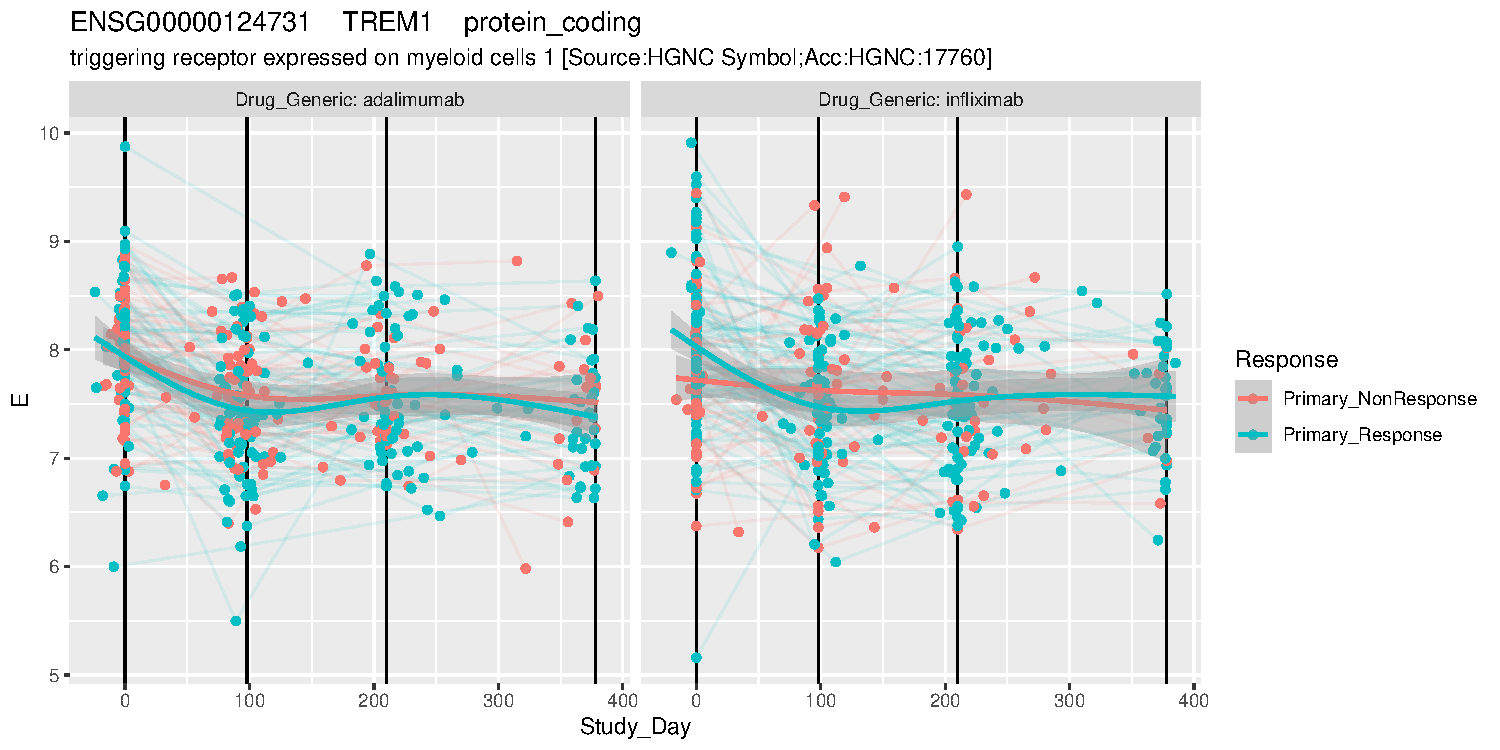
\includegraphics[width=1.0\textwidth,page=1]{mainmatter/figures/chapter_04/dream.E_vs_Study_Day.GENEID_ENSG00000124731.SYMBOL_TREM1.pdf}
%     \caption{Unadjusted, normalised TREM1 expression over time}
%     \label{fig:multipants_dge_TREM1}
% \end{figure}

\subsection{Post-induction gene expression associated with primary response}

The same methodology applied at week 0 was applied at week 14 to identify differences in post-induction expression associated with primary response.
A larger proportion of the transcriptome is differentially expressed between responders and non-responders at week 14: 
1364 for the infliximab-only comparison, 
1544 for the adalimumab-only comparison, 
and 4841 pooling both drugs (\cref{fig:multipants_dge_volcano_week_14_R_N}).
No significant interactions between drug and response were detected at the per-gene level.
Given that sample sizes at week 0 and week 14 are comparable (\cref{fig:multipants_studyDay_boxplots}), the overall signal-to-noise ratio is much stronger than at baseline.

Adjusting for cell composition, 1320/1364, 1515/1544 and 4653/4841 genes have dampened effects;
% \todo{Carl's comment: And does this include genes that are no longer significantly differentially expressed. I would find helpful to know how many genes are no longer eGenes, and how many remain eGenes but where the eQTL has a lower effect.}
% NOTE: mag, damp, flip only counts signs, not signif
and the numbers of significant genes drop to 379, 177, and 1302 for infliximab, adalimumab, and pooled analyses respectively.
This again suggests many effects are mediated by differences in immune cell composition between responders and non-responders.

% TODO: add module names
Modules including generic immune activation, monocytes, TLR and inflammatory signalling, and neutrophils were downregulated in responders; 
whereas B cell and plasma cell modules were upregulated (\cref{fig:multipants_dge_panelPlot_week_14_R_N_cellPropF}).
These modules remained differentially expressed with the same direction of effect after adjusting for cell composition (\cref{fig:multipants_dge_panelPlot_week_14_R_N_cellPropT}), 
suggesting there is per-cell up or downregulation on top of abundance changes of the cell types expressing these modules.
% \todo{Carl's comment: I take it that the changes in abundance match the direction of effect of the expression change. I guess they must but it would be good to check this.}
Modules related to antigen presentation (LI.M71, LI.M97.0, LI.M5.0),
interferon (LI.M75, LI.M127, LI.M111.1),
and dendritic cells (LI.M64, LI.M165)
also appear among significantly downregulated modules after cell composition adjustment.
Directions of effect for the most significant modules were largely consistent between drugs, 
and there are few significant drug by response interaction effects
This is in contrast to the baseline responder vs. non-responder comparison,
where many of the strongest effects in the pooled analysis were driven by stronger effects in one drug.

\gene{SIGLEC10} from the baseline analysis retains its significant association with primary response post-induction, 
with the same direction of effect (adjusted $\log_2\text{\gls{FC}} = \num{0.36610032}$).
% \todo{highlight a few more individual genes specific to this analysis too? not sure how to pick them at the moment.}
Some genes previously proposed as baseline markers of response in gut mucosa: \gene{G0S2}, \gene{TNFAIP6}, \gene{S100A8} and \gene{S100A9} by \textcite{arijs2010PredictiveValueEpithelial}; and \gene{OSM} by \textcite{west2017OncostatinDrivesIntestinal},
were differentially expressed in post-induction blood in this study.
The direction of effect for both sets of markers, downregulation in primary responders, also matches this study.

\begin{figure}
    \centering
    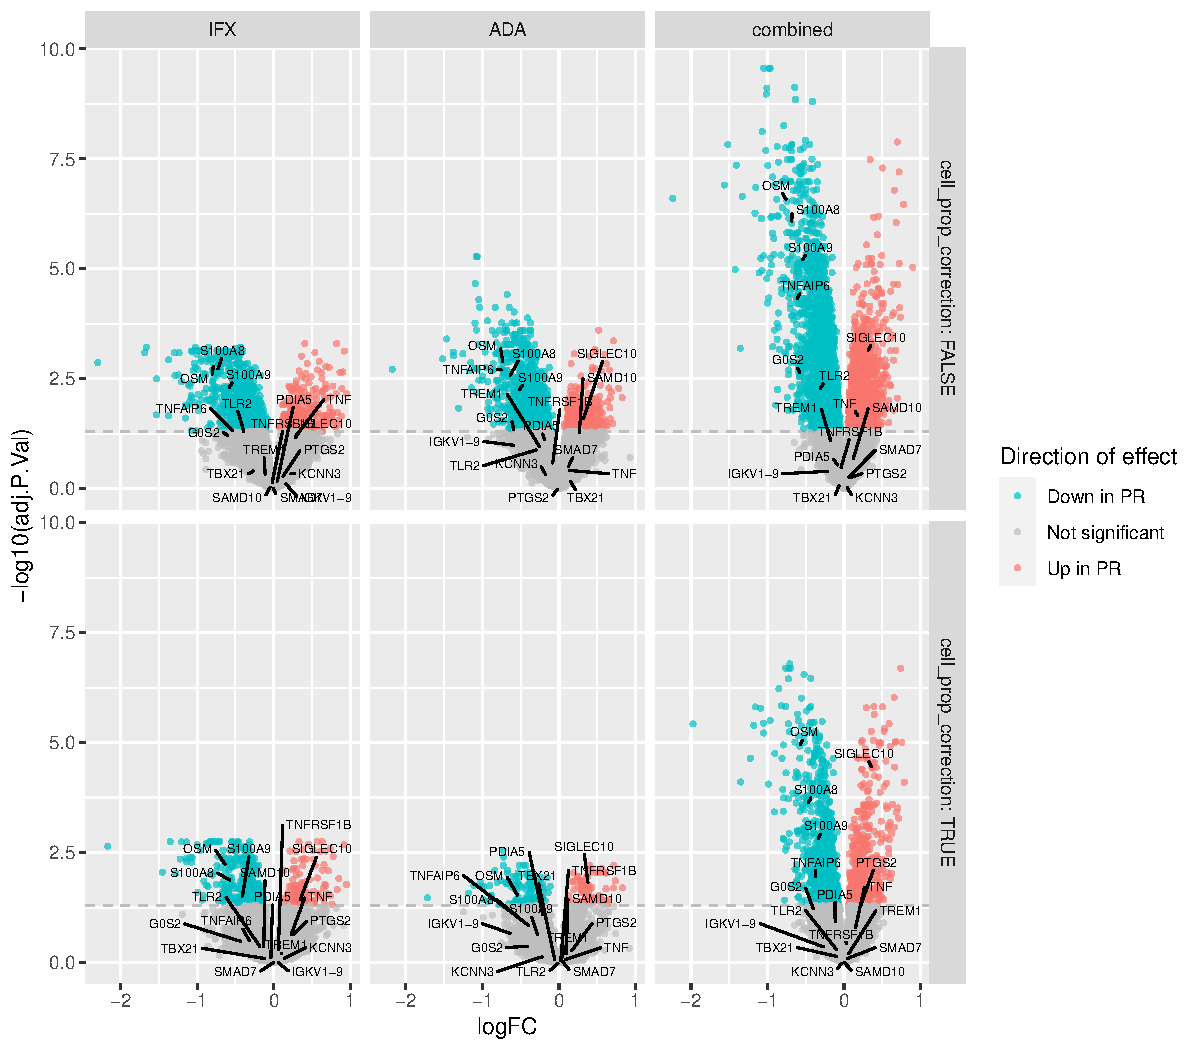
\includegraphics[width=1.0\textwidth,page=1]{mainmatter/figures/chapter_04/plot_gene_set_enrichment.dge_result_volcano_simple_C_3RI_3NI,C_3RA_3NA,C_3R_3N.pdf}
    \caption{
        \textbf{Volcano plots of \gls{DGE} between primary responders and non-responders at week 14; unadjusted (top row) and adjusted (bottom row) for cell composition; for infliximab (IFX), adalimumab (ADA), or with both drugs pooled.}
        Annotated genes include significant associations from this study and previously reported associations from \autoref{subsec:multiPANTS_intro_predicting_response}.
        Dashed line shows significance threshold at FDR = 0.05.
        PR = primary responder.
    }
    \label{fig:multipants_dge_volcano_week_14_R_N}
\end{figure}

\begin{figure}
    \centering
    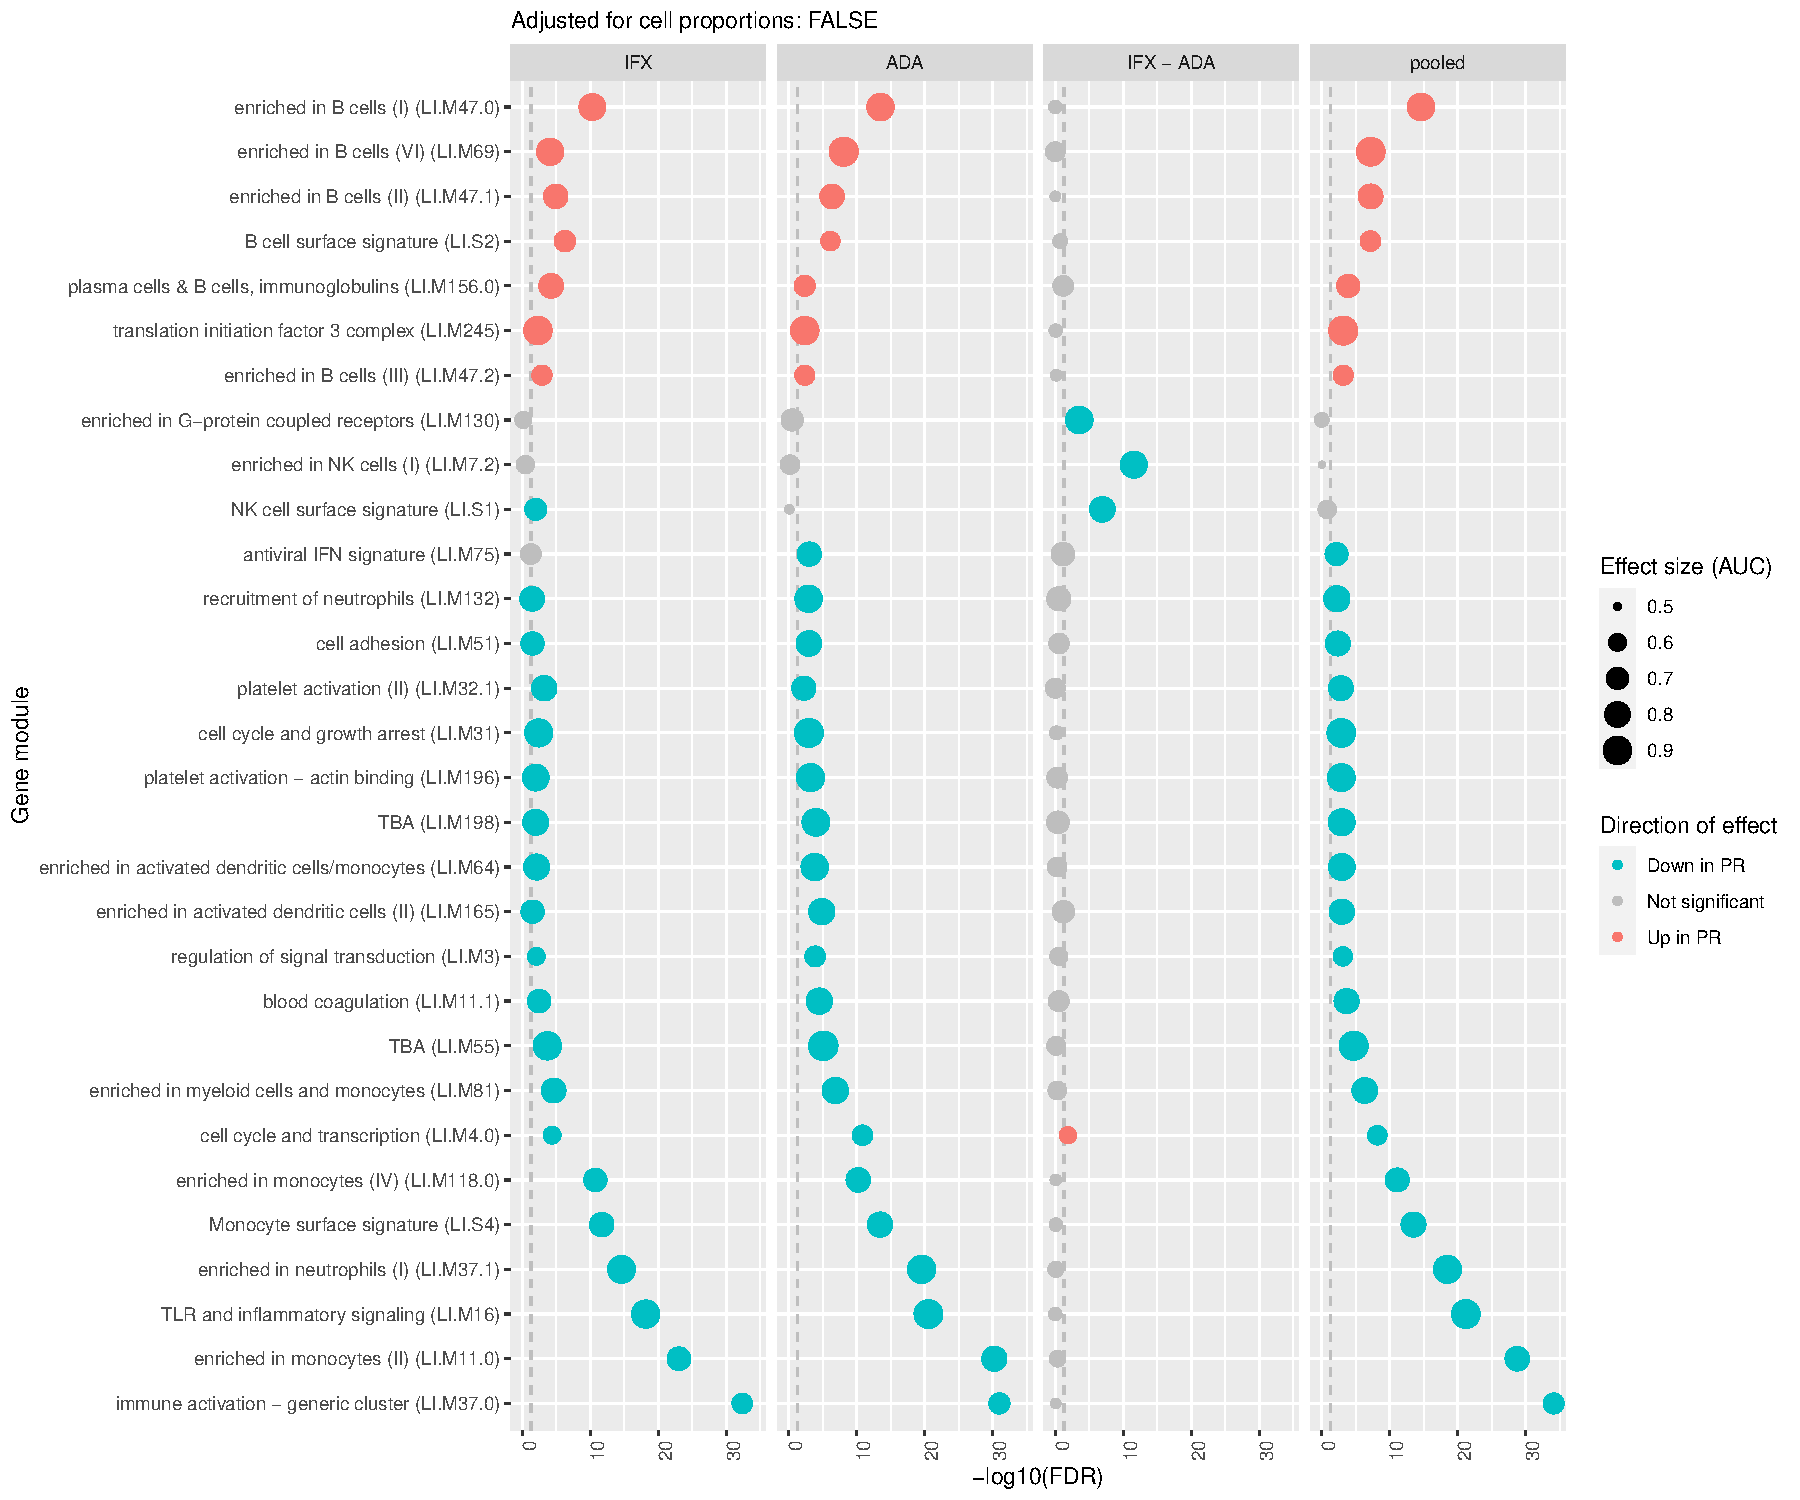
\includegraphics[width=1.0\textwidth,page=1]{mainmatter/figures/chapter_04/plot_gene_set_enrichment.tmodCERNO_panelplot_reversed_C_3RI_3NI,C_3RA_3NA,C_(3RI_3NI)_(3RA_3NA),C_3R_3N.cell_prop_correction_FALSE.pdf}
    \caption{
        \textbf{Top modules differentially expressed between primary responders and non-responders at week 14, unadjusted for cell composition.}
        Columns correspond to results from infliximab (IFX), adalimumab (ADA), infliximab-adalimumab difference and pooled analyses. 
        The top 30 modules ranked by minimum \gls{FDR} in any column are shown. Vertical dashed line shows significance threshold at FDR = 0.05.
        PR = primary responder.
    }
    \label{fig:multipants_dge_panelPlot_week_14_R_N_cellPropF}
\end{figure}

\begin{figure}
    \centering
    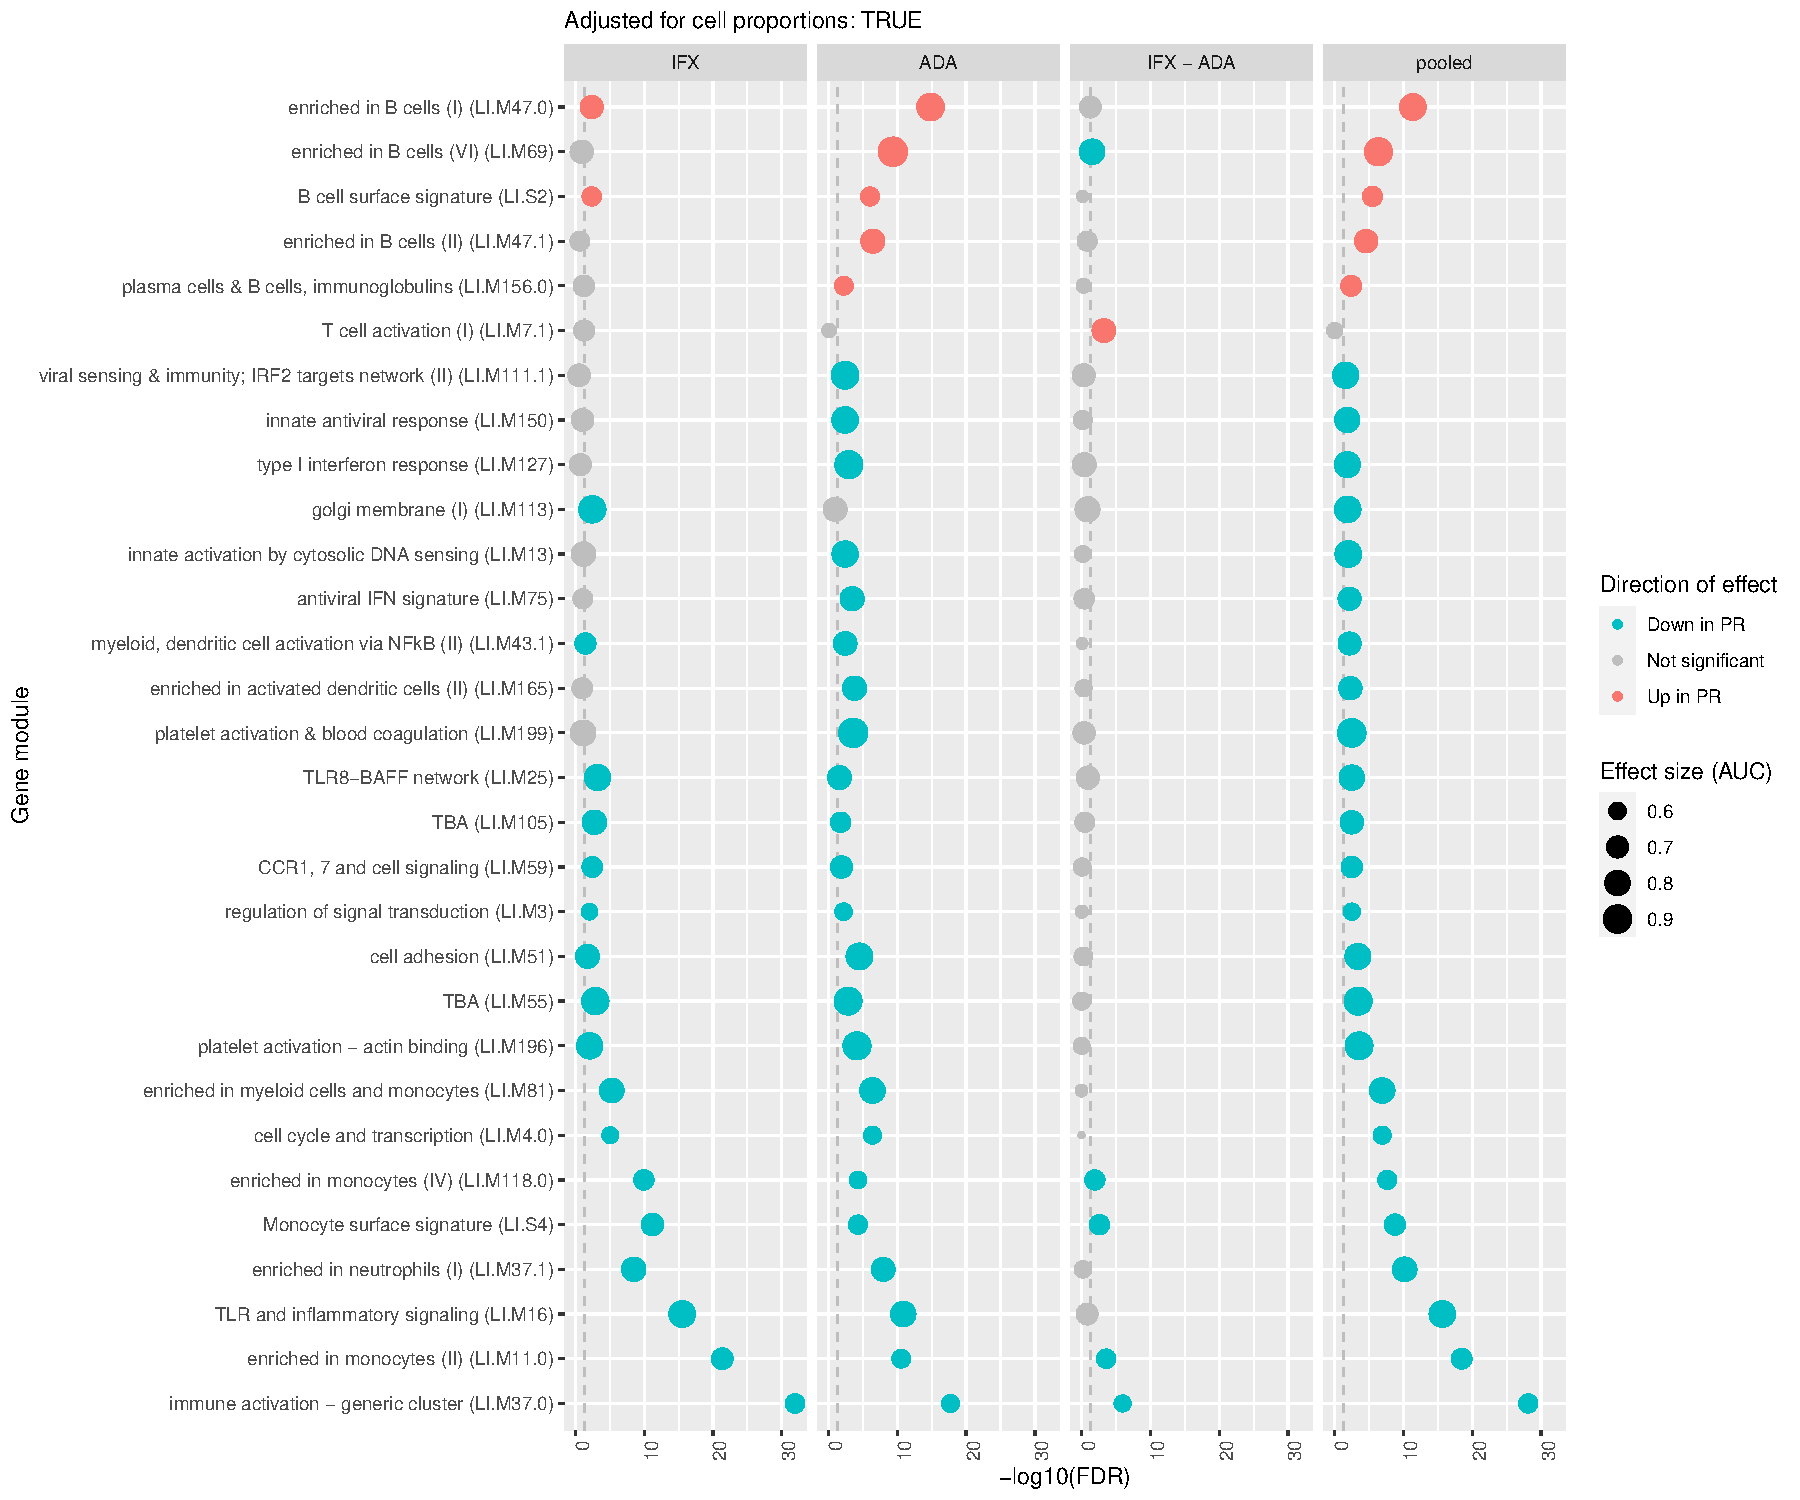
\includegraphics[width=1.0\textwidth,page=1]{mainmatter/figures/chapter_04/plot_gene_set_enrichment.tmodCERNO_panelplot_reversed_C_3RI_3NI,C_3RA_3NA,C_(3RI_3NI)_(3RA_3NA),C_3R_3N.cell_prop_correction_TRUE.pdf}
    \caption{
        \textbf{Top modules differentially expressed between primary responders and non-responders at week 14, adjusted for cell composition.}
        Columns correspond to results from infliximab (IFX), adalimumab (ADA), infliximab-adalimumab difference and pooled analyses. 
        The top 30 modules ranked by minimum \gls{FDR} in any column are shown. Vertical dashed line shows significance threshold at FDR = 0.05.
        PR = primary responder.
    }
    \label{fig:multipants_dge_panelPlot_week_14_R_N_cellPropT}
\end{figure}

\subsection{Magnification of expression change from baseline to post-induction in responders}

Given the stronger differences in expression between primary responders and non-responders at week 14 versus week 0,
I estimated the change in expression from week 0 to week 14 within the two groups, and also estimated the timepoint by response interaction.
I perform only the pooled comparison here both to simplify the analysis, and because similarly to the within week 14 comparison, change from week 0 to week 14 was relatively consistent between drugs, with exceptions noted.

Without adjusting for cell composition,
12862 genes were differentially expressed in primary responders at week 14 vs week 0 in the pooled analysis,
8310 genes in primary non-responders,
and 6320 genes had a significant interaction.
After adjusting for cell composition, 
5572 genes were differentially expressed in primary responders,
626 genes in primary non-responders,
and 179 genes had a significant interaction.
Of the genes differentially expressed between week 14 and week 0 in both primary responders and non-responders,
and with a significant interaction between timepoint and response, 
nearly all (4885/4891 unadjusted for cell composition, 31/32 adjusted) were magnified by primary response i.e.
the same genes have larger fold-changes in the same direction for primary responders (\cref{fig:multipants_dge_logFC_C_3R_1R_vs_logFC_C_3N_1N}).

\begin{figure}
    \centering
    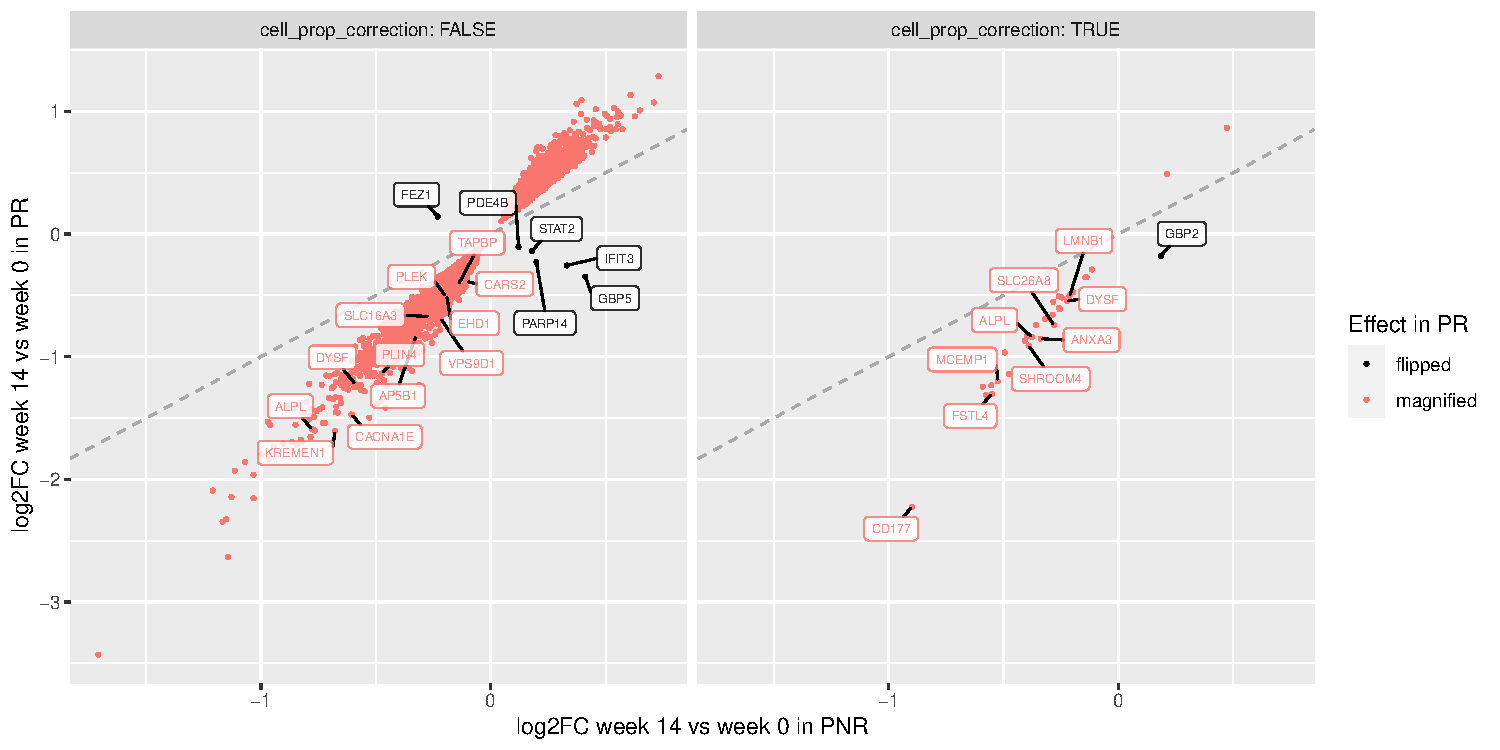
\includegraphics[width=1.0\textwidth,page=1]{mainmatter/figures/chapter_04/plot_gene_set_enrichment.logFC_C_3R_1R_vs_logFC_C_3N_1N.pdf}
    \caption{
        \textbf{Expression $\log_2\text{\gls{FC}}$ from week 0 to week 14 in primary responders (PR) versus non-responders (PNR),
        for genes that are differentially expressed from week 0 to week 14 in both responders and non-responders, with a significantly different effect size in responders and non-responders.
        }
        Results adjusted (right) and unadjusted (left) for cell proportions are shown.
        Identity line shown by dashed line.
        Most expression changes from week 0 to week 14 are magnified in primary responders, with a small proportion of changes in the opposite direction.
    }
    \label{fig:multipants_dge_logFC_C_3R_1R_vs_logFC_C_3N_1N}
\end{figure}

% NOTE: choosing these to be present in both drugs and pooled
The most significant modules that change from week 0 to week 14 in responders included
upregulation of B cell (LI.M47.0), plasma cell (LI.M156.0), and T cell activation (LI.M7.1);
and downregulation of immune activation (LI.M37.0), monocyte (LI.M11.0), neutrophil (LI.M37.1) and TLR and inflammatory signalling (LI.M16) modules (\cref{fig:multipants_dge_panelPlot_week_14_0_R_N_cellPropF}).
% Many of these are the same modules associated with response within the week 0 and week 14 timepoints.
Many of these are the same modules associated with response within the week 14 timepoint, and in the same direction (\cref{fig:multipants_dge_panelPlot_week_14_R_N_cellPropF}),
suggesting that a change in expression of these gene sets from week 0 to week 14 is what leads to the difference between responders and non-responders at week 14.
% TODO what about the week 0 timepoint? recheck it
% \todo{Carl's comment: So one is more likely to be a responder if you are highly expressing genes in the gene-sets at baseline and/or you have a large up-regulation of these genes by week14?}

Adjusting for cell composition decreases the significance of a majority of modules (\cref{fig:multipants_dge_panelPlot_week_14_0_R_N_cellPropT}),
with T cell modules in the adalimumab-only analysis especially decreased.
Magnification is also observed at the module level, with nearly all module effects aligned in the same direction in responders and non-responders, with significant interactions also in the same direction.
In general, responders seem to experience greater changes in their gene expression from week 0 to week 14 due to the drug.

\begin{figure}
    \centering
    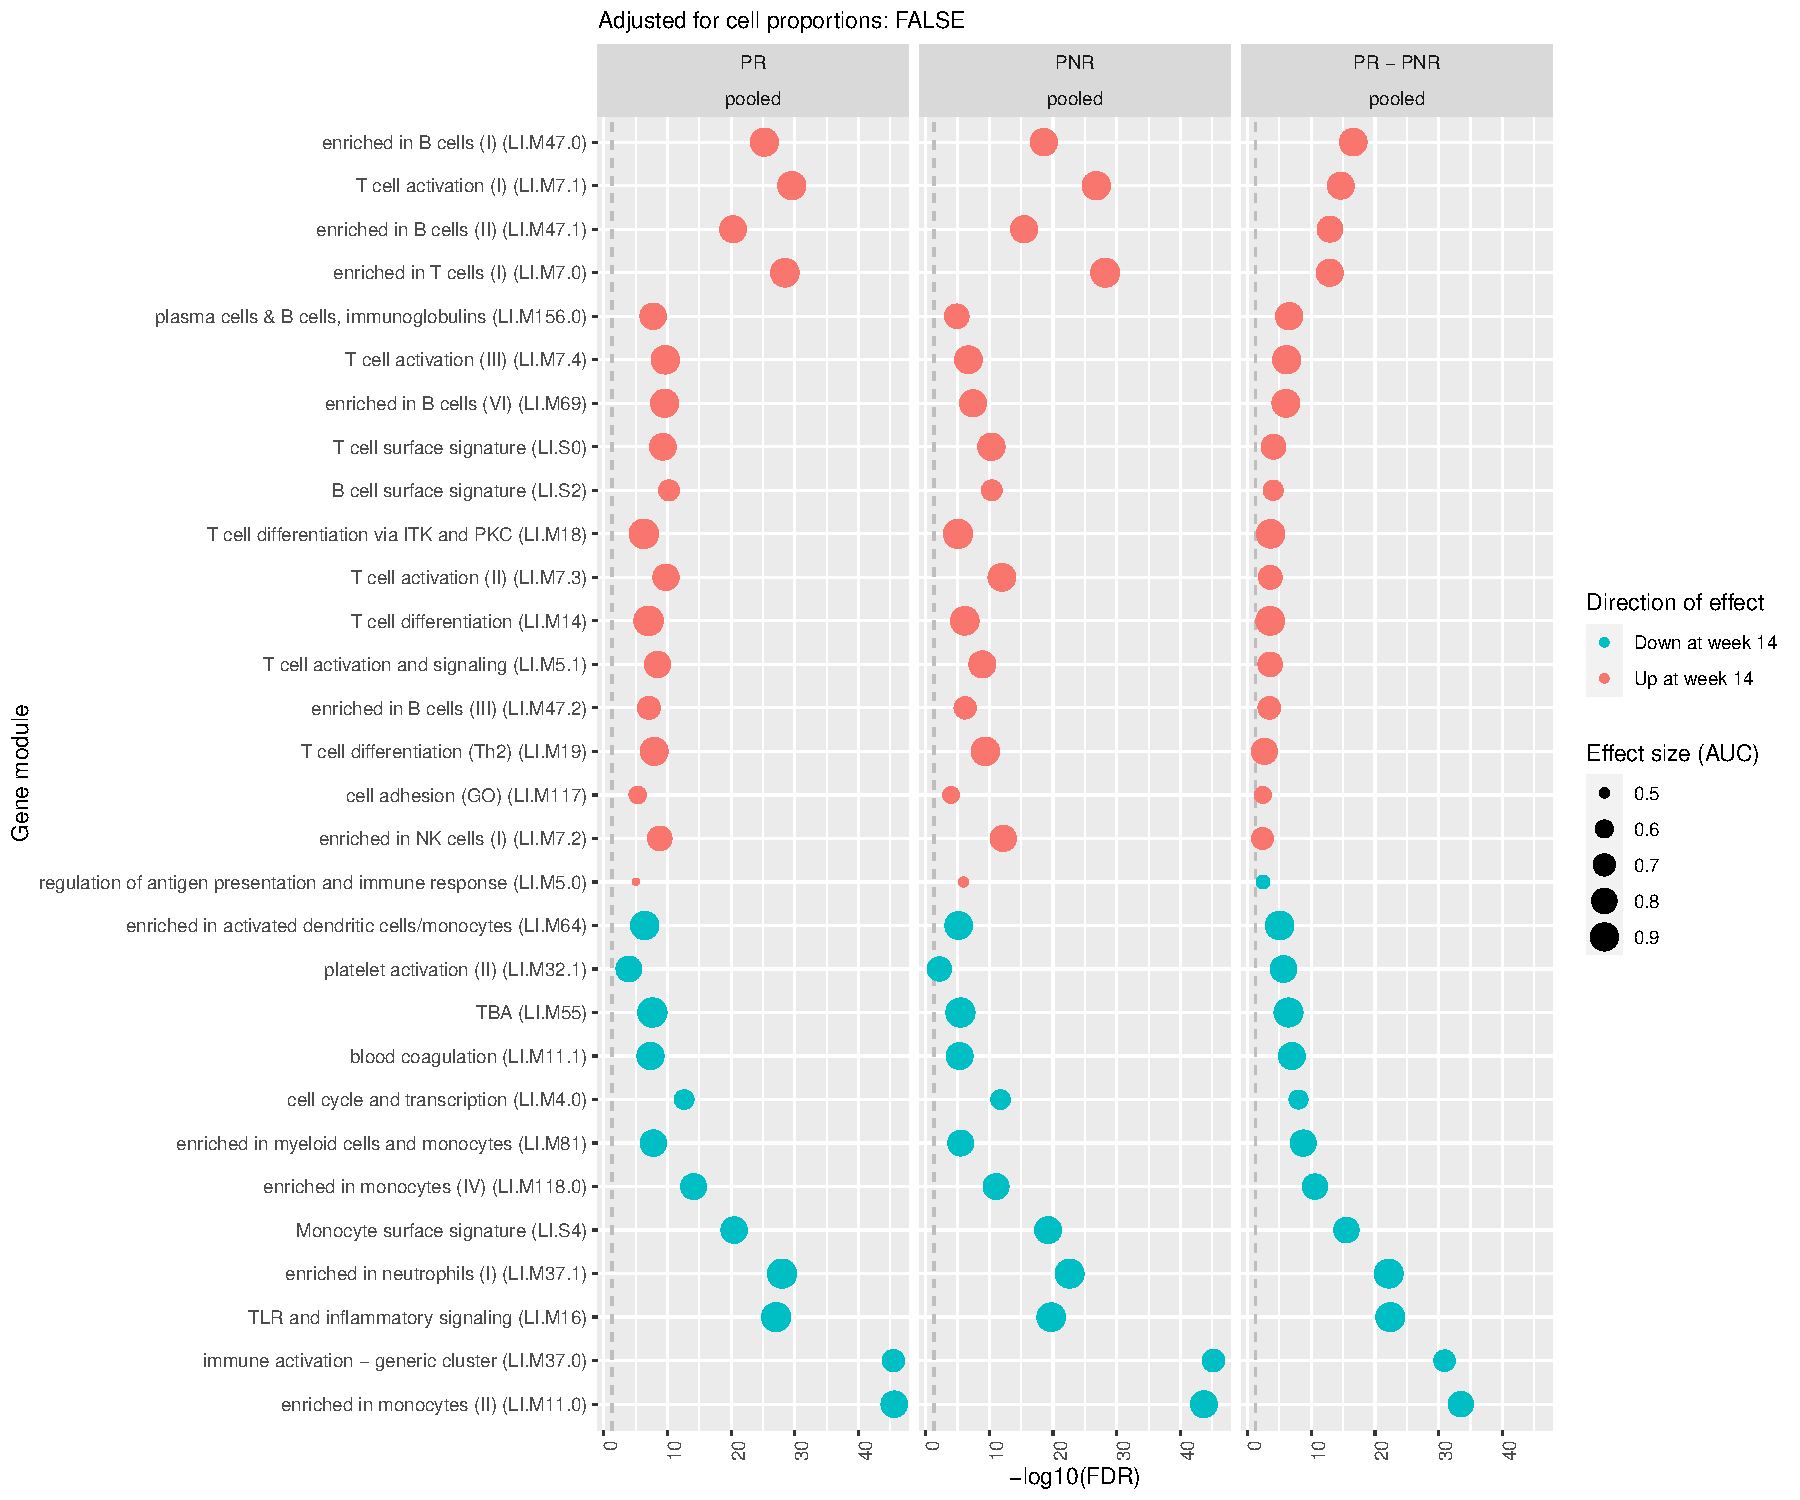
\includegraphics[width=1.0\textwidth,page=1]{mainmatter/figures/chapter_04/plot_gene_set_enrichment.tmodCERNO_panelplot_reversed_C_3R_1R,C_3N_1N,C_(3R_1R)_(3N_1N).cell_prop_correction_FALSE.pdf}
    \caption{
        \textbf{Top modules differentially expressed between week 14 and week 0, unadjusted for cell composition.}
        Columns show effects in primary responders (PR), non-responders (PNR), and the primary responder minus non-responder difference. 
        The top 30 modules ranked by minimum \gls{FDR} in any column are shown. 
        Vertical dashed line shows significance threshold at FDR = 0.05.
    }
    \label{fig:multipants_dge_panelPlot_week_14_0_R_N_cellPropF}
\end{figure}

\begin{figure}
    \centering
    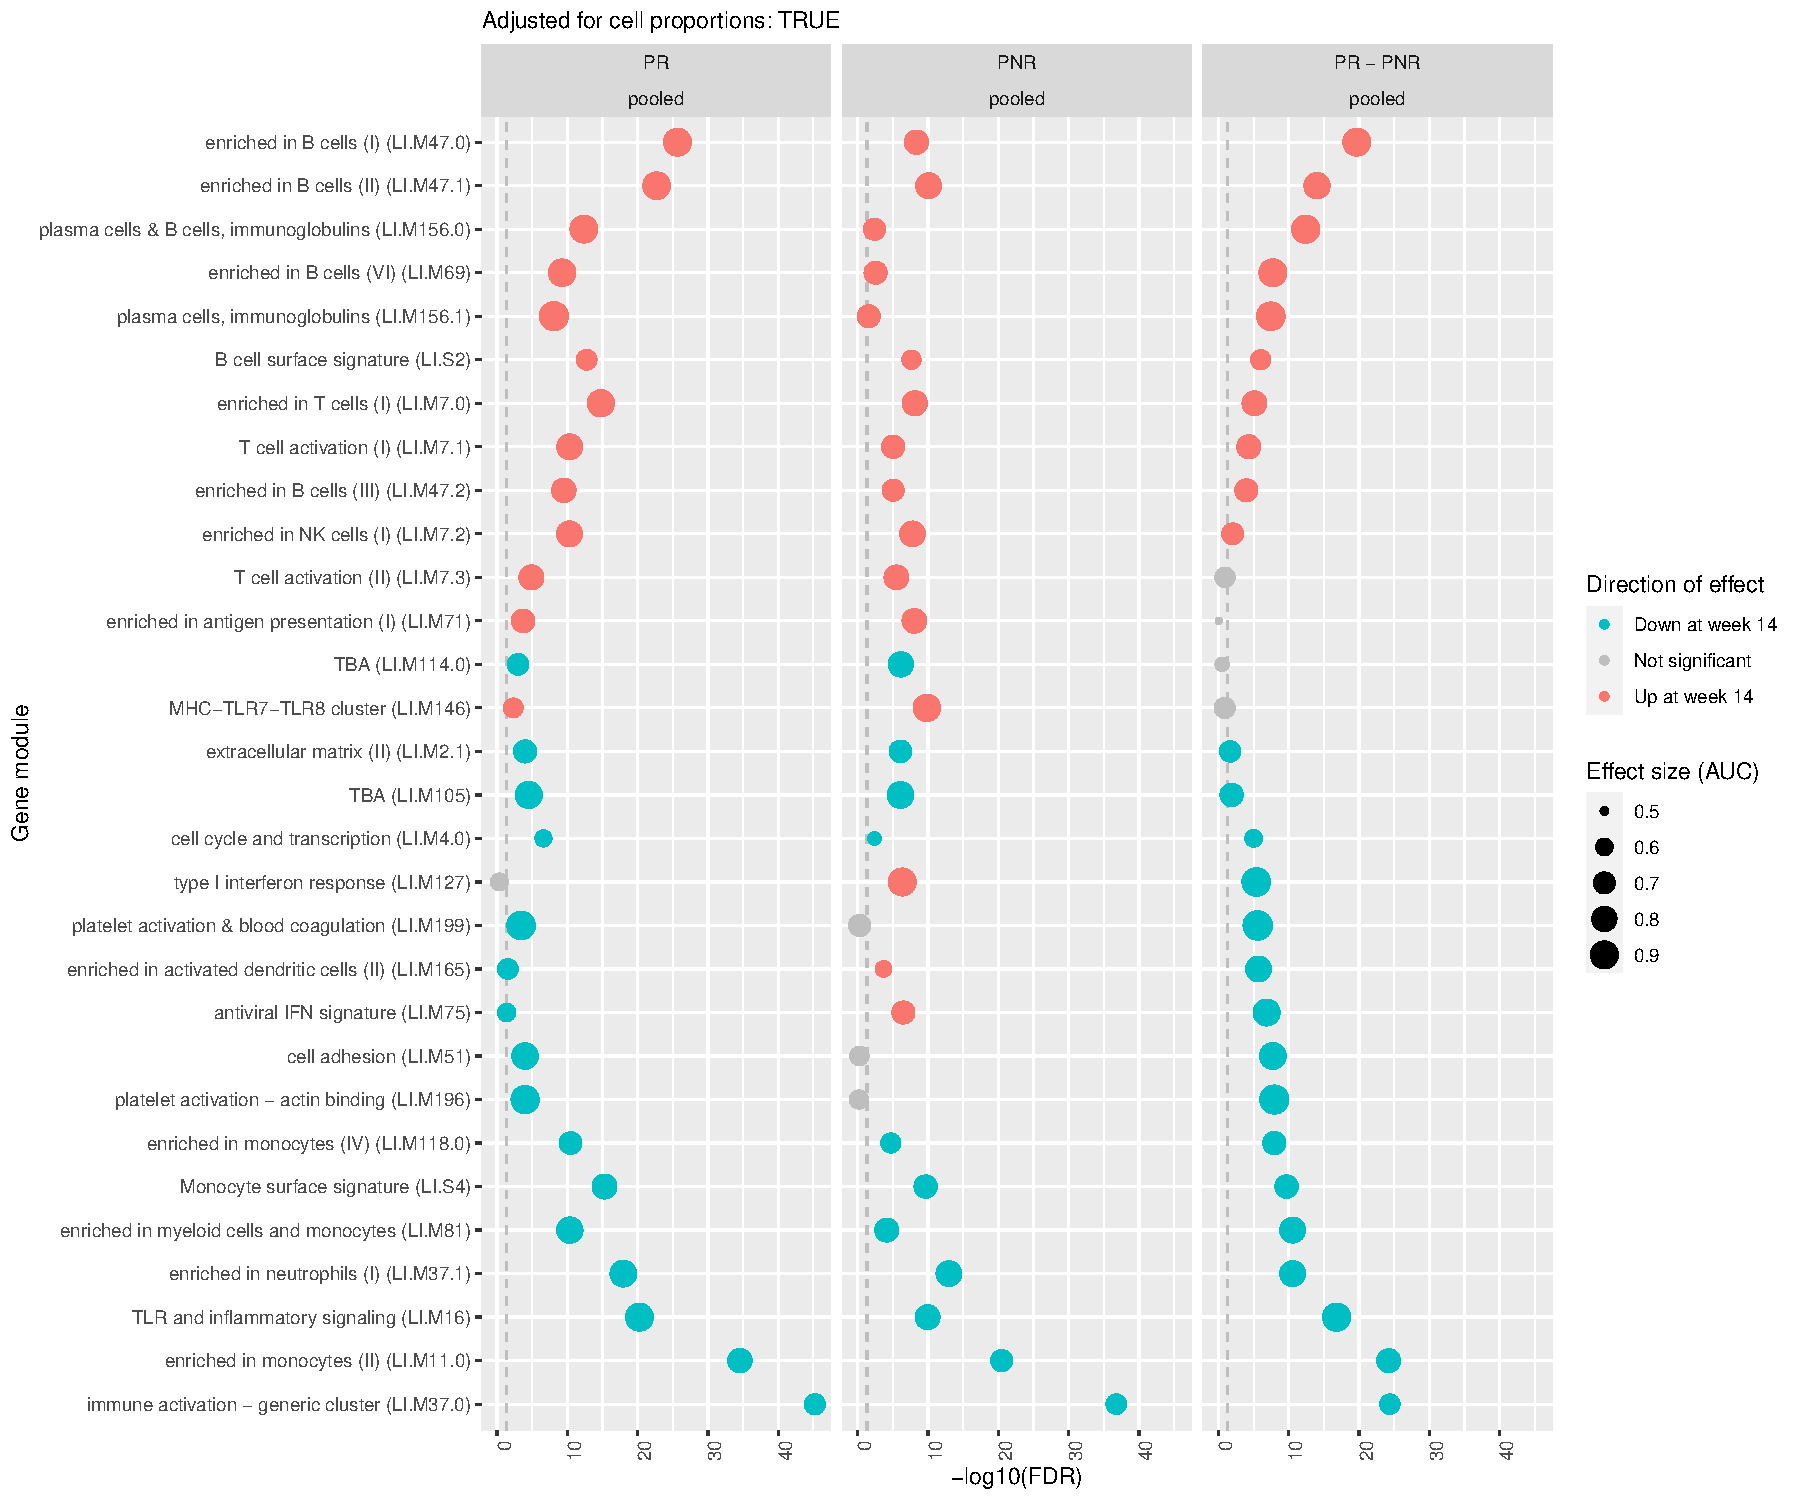
\includegraphics[width=1.0\textwidth,page=1]{mainmatter/figures/chapter_04/plot_gene_set_enrichment.tmodCERNO_panelplot_reversed_C_3R_1R,C_3N_1N,C_(3R_1R)_(3N_1N).cell_prop_correction_TRUE.pdf}
    \caption{
        \textbf{Top modules differentially expressed between week 14 and week 0, adjusted for cell composition.}
        Columns show effects in primary responders (PR), non-responders (PNR), and the primary responder minus non-responder difference. 
        The top 30 modules ranked by minimum \gls{FDR} in any column are shown. 
        Vertical dashed line shows significance threshold at FDR = 0.05.
    }
    \label{fig:multipants_dge_panelPlot_week_14_0_R_N_cellPropT}
\end{figure}

\subsection{Interferon modules with opposing differential expression in responders and non-responders}
\label{subsec:multipants_dge_opposing_interferon}

\cref{fig:multipants_dge_logFC_C_3R_1R_vs_logFC_C_3N_1N} also contains genes that were downregulated from week 0 to week 14 in responders, but upregulated in non-responders (\enquote{flipped}).
% TODO: unify terminology with ch3
At the module level these opposing effects were most apparent after cell composition adjustment for 
antiviral interferon signature (LI.M175), type I interferon response (LI.M127), and antigen presentation (LI.M95.0) (\cref{fig:multipants_dge_panelPlot_week_14_0_R_N_cellPropT}).
I extended my module analysis to include modules from \autocite{chaussabel2008ModularAnalysisFramework} (prefixed \enquote{DC}).
Although these modules are on the whole poorly annotated compared to modules from \autocite{li2013MolecularSignaturesAntibody}, interferon modules are annotated.
% tmodHGtest FDR=\num{0.0001261719}
\gene{STAT2}, \gene{GBP5}, and \gene{PARP14} from \cref{fig:multipants_dge_logFC_C_3R_1R_vs_logFC_C_3N_1N} are annotated into an interferon module (DC.M3.4).
\gene{IFIT3} and \gene{GBP2} are also annotated into separate interferon modules (DC.M1.2, DC.M5.12).
Adjusted for cell composition, these modules are all significantly upregulated at week 14 in non-responders only: 
DC.M3.4 (FDR=\num{3.446797e-21}),
DC.M1.2 (FDR=\num{9.492256e-16}),
and DC.M5.12 (FDR=\num{1.355467e-13})
(\cref{fig:multipants_dge_evidencePlots_C_3_1_Interferon}).

\begin{figure}
    \centering
    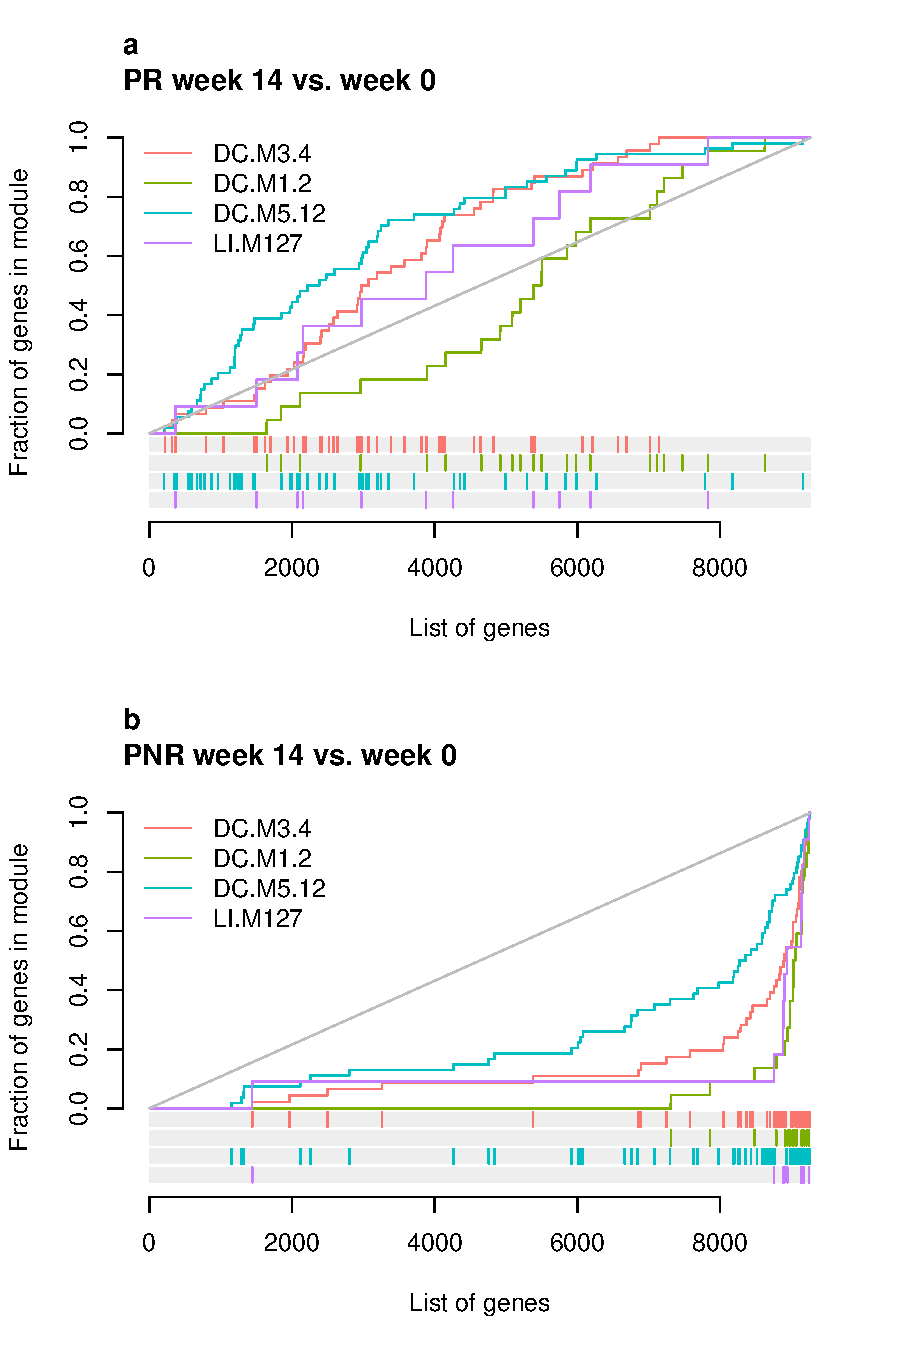
\includegraphics[width=0.8\textwidth,page=1]{mainmatter/figures/chapter_04/plot_gene_set_enrichment.evidencePlots_C_3_1_Interferon.pdf}
    % TODO: only 8-9k genes
    % TODO: add module names
    \caption{
        \textbf{\software{tmod} evidence plots showing interferon-related modules specifically upregulated from week 0 to week 14 in primary non-responders.}
        Genes were ranked in ascending order by week 14 versus week 0 \gls{DGE} z-statistic. 
        The ranks of genes in interferon-related modules are indicated by colored rug plots. 
        Colored curves show the cumulative fraction of genes in each module. 
        For non-responders, these modules are enriched for large ranks (large, positive $z$-statistics). 
        The area under the colored curves are the effect sizes (\glspl{AUC}). 
        The null of randomly-distributed ranks is the grey diagonal line.
        PR = primary responder, PNR = primary non-responder.
    }
    \label{fig:multipants_dge_evidencePlots_C_3_1_Interferon}
\end{figure}

\subsection{Sustained expression differences between primary responders and non-responders during maintenance}

As \gls{PANTS} is an observational study, it was able to include some patients who continued with anti-\gls{TNF} therapy
even after meeting the definition of primary non-response at week 14.
For both responders and non-responders, expression data was also available from blood samples around week 30 and week 54, and at additional visits scheduled in the event of secondary LOR.

I fit a natural cubic spline to the expression of each gene as a function of study day, and tested for general differences in expression over time between responders and non-responders.
This analysis was performed only with drugs pooled due to lower sample sizes for later timepoints.
Without adjusting for cell composition, 
4426 genes were differentially expressed between responders and non-responders;
210 genes were differentially expressed after adjustment.
To identify distinct trajectories of expression over time, I hierarchically clustered those 210 genes by
their mean expression in responders and non-responders at each timepoint, 
and determined the optimal number of clusters by the gap statistic method (\cref{fig:multipants_dge_spline_fviz_nbclust_gap_stat}).
Six distinct clusters were proposed (\cref{fig:multipants_dge_spline_cluster_trajectories}).

\begin{figure}
    \centering
    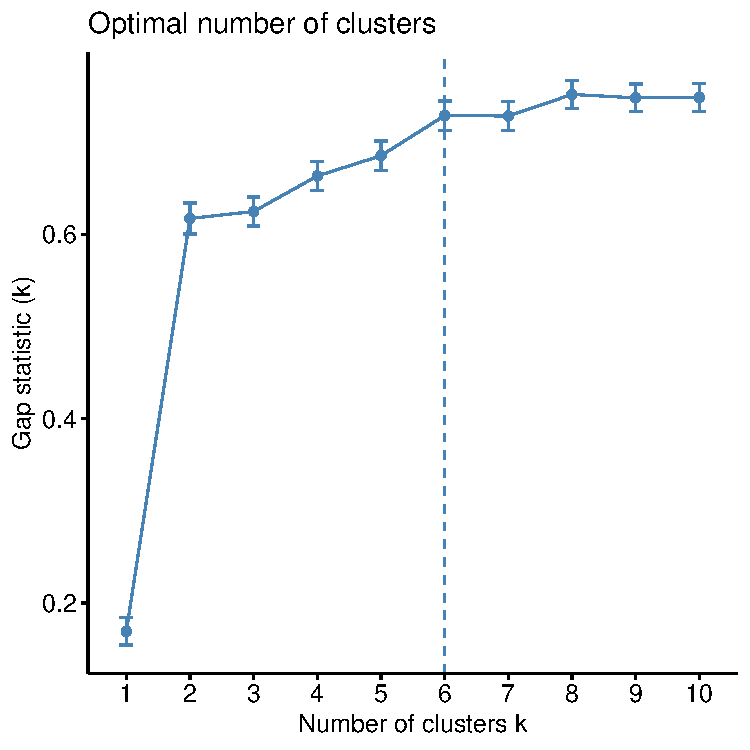
\includegraphics[width=1.0\textwidth,page=1]{mainmatter/figures/chapter_04/plot_gene_set_enrichment.spline_fviz_nbclust_gap_stat.pdf}
    \caption{
        \textbf{Gap statistic versus cluster number $k$.}
        Error bars derived from 500 bootstraps. 
        The optimal number of clusters is defined as the smallest $k$ where Gap($k$) is greater than the lower bound of Gap($k+1$) \autocite{tibshirani2001EstimatingNumberClusters}.
        Here, the optimal $k$ is six.
    }
    \label{fig:multipants_dge_spline_fviz_nbclust_gap_stat}
\end{figure}

\begin{figure}
    \centering
    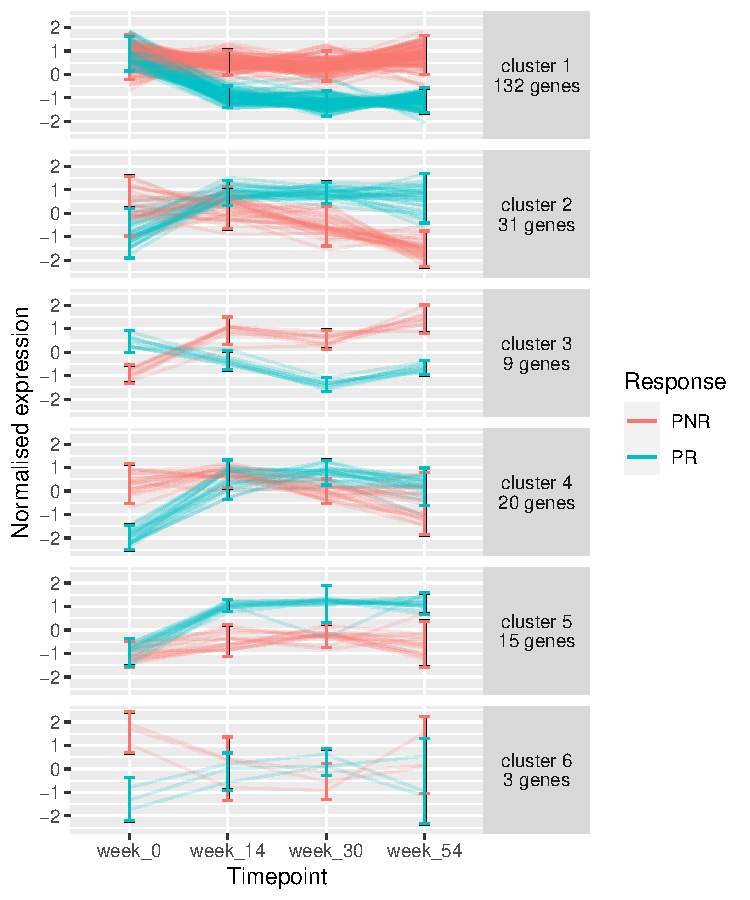
\includegraphics[width=1.0\textwidth,page=1]{mainmatter/figures/chapter_04/plot_gene_set_enrichment.spline_cluster_trajectories.pdf}
    \caption{
        \textbf{Normalised expression over the timepoints for genes in the six identified clusters.}
        Log scaled expression for each gene was standardised before clustering.
        Error bars are the expression mean and standard deviation for the genes at each timepoint in primary responders and non-responders.
        PR = primary responder, PNR = primary non-responder.
    }
    \label{fig:multipants_dge_spline_cluster_trajectories}
\end{figure}

Many of these genes had previously been identified as having significant differences in expression between responders and non-responders
either within week 14, or for change in expression from week 0 to week 14.
Cluster 1 contained mainly previously identified genes (\cref{fig:plot_gene_set_enrichment.spline_cluster_venns.pdf}),
and was enriched for modules including 
myeloid cells and monocytes (LI.M81, hypergeometric test, FDR=\num{2.114861e-06}),
platelet activation (LI.M196, FDR=\num{1.347609e-05}),
immune activation (LI.M37.0, FDR=\num{1.435659e-04}),
and TLR and inflammatory signalling (LI.M16, FDR=\num{2.364913e-03}).
The spline analysis highlighted that expression differences at week 14 are maintained at week 30 and week 54.

\begin{figure}
    \centering
    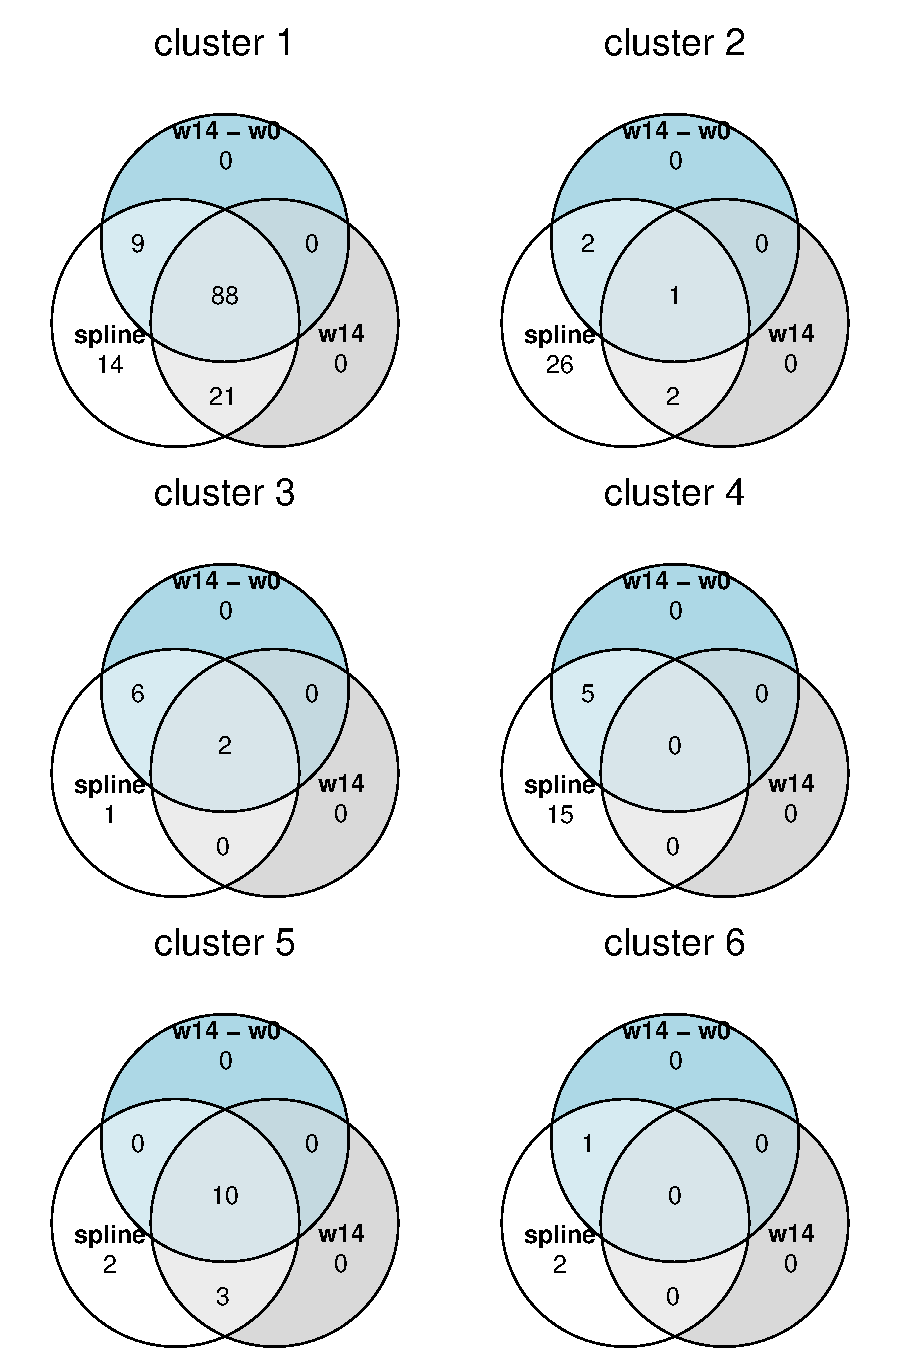
\includegraphics[width=0.8\textwidth,page=1]{mainmatter/figures/chapter_04/plot_gene_set_enrichment.spline_cluster_venns.pdf}
    \caption{
        \textbf{Venn diagrams showing which genes in each spline cluster were also significant in the week 14 responder versus non-responder contrast (w14), or the interaction between week 0 to week 14 change and response status (w14-w0).}
    }
    \label{fig:plot_gene_set_enrichment.spline_cluster_venns.pdf}
\end{figure}

The highest proportion of genes uniquely identified as significant by the spline analysis were in cluster 2 (26/31) and cluster 4 (15/20).
Cluster 2 was enriched in \autocite{li2013MolecularSignaturesAntibody} B cell modules (LI.M47.0, FDR=\num{1.525815e-06}; LI.M47.1, FDR=\num{4.531246e-05})
previously identified as having a greater increase from week 0 to week 14 in primary responders versus primary non-responders (\cref{fig:multipants_dge_panelPlot_week_14_0_R_N_cellPropT}),
matching the observed cluster trajectory.
Cluster 4 was not enriched in any modules from \textcite{li2013MolecularSignaturesAntibody}, but is enriched for a B cell module (DC.M4.10, FDR=\num{0.001367196}) from \textcite{chaussabel2008ModularAnalysisFramework}.
Although no genes were significantly associated with response at week 0 (\cref{fig:multipants_dge_volcano_week_0_R_N}),
the genes in cluster 4 are coordinately downregulated as a set in primary responders (CERNO test, p=\num{6.175642e-25}).

% AL353807.3
% STAT1
% BATF2
% GBP1
% GBP5
% IRF1
% TAP1
% APOL2
% APOL1
Cluster 3 is also of interest, enriched for type I interferon response (LI.M127, FDR=\num{0.005680666}) and interferon (DC.M3.4, FDR=\num{0.0005266239}) modules,
as well as genes that contain putative transcription factor binding motifs for interferon regulatory factors \gene{IRF7} ({g:Profiler} term ID TF:M00453\_1, adj. p value=\num{0.0050514484}) 
and \gene{IRF8} (TF:M11684\_1, adj. p value=\num{0.0077680709}; TF:M11685\_1, adj. p=\num{0.0103433288}).
The cluster trajectory shows direction of expression change is opposing in responders and non-responders from week 0 to week 14, followed by sustained differences at week 30 and week 54.
The trajectory and interferon-related gene set enrichments are consistent with those identified in \cref{subsec:multipants_dge_opposing_interferon}.
Of the 9 genes in this cluster, 8 genes (\gene{STAT1}, \gene{BATF2}, \gene{GBP1}, \gene{GBP5}, \gene{IRF1}, \gene{TAP1}, \gene{APOL1}, \gene{APOL2})
have significant interaction between week 0 to week 14 expression change and response status,
whether or not correcting for cell composition.
However, only \gene{GBP5} was differentially expressed from week 0 to week 14 in both responders and non-responders,
and only when unadjusted for cell composition (\cref{fig:multipants_dge_logFC_C_3R_1R_vs_logFC_C_3N_1N}).
This indicates that such small and opposite effects in responders and non-responders are best detected at a single-gene level in the interaction analysis that tests the difference,
and in the spline analysis, with the support of additional data from week 30 and week 54.

% TODO: add siglec 10 trend raw, and add to discussion
    
\subsection{Limited evidence for change in genetic architecture of gene expression over time}

Given the substantial changes in expression from baseline to post-induction after starting the drug, and the differing trajectories observed in responders and non-responders, 
I performed \gls{eQTL} mapping to identity common genetic variants associated with expression that may contribute to these differences.
Variants \textit{cis} (within \SI{1}{\mega b} of the TSS) to 15040 genes were tested for association.
Mapping was performed within each timepoint (weeks 0, 14, 30, and 54),
followed by joint analysis of per-timepoint \gls{eQTL} summary statistics and control for multiple testing using \software{mashr}.

% TODO
% also drugs pooled due to much more power for eqtl required than DGE, may be inappropriate

% TODO: see https://www.nature.com/articles/nature24277#Sec5
% for classic U-curve for sharing

The majority 11156/15040 (\percentage{0.74175531914}) of genes were eGenes (a gene with at least one significant \textit{cis}-\gls{eQTL}) in at least 1 timepoint (\gls{lfsr} < 0.05).
The variant with the lowest \gls{lfsr} over all timepoints for each gene was 
chosen as the lead variant (eSNP) for that gene.
Most eSNPs were significant in multiple timepoints: 999 significant in 1 timepoint, 381 significant in 2 timepoints, 526 significant in 3 timepoints, 9250 significant in all 4 timepoints.
I compared eSNP effect sizes between week 0 and each of weeks 14, 30 and 54,
to identify \glspl{reQTL} with significant difference in effect versus baseline,
as they may also explain changes in expression from baseline.
Most eSNPs were shared across timepoints;
only six eSNPs-eGene pairs were significant at BH FDR < 0.05:
with 1/6 for week 30 versus week 0 and 5/6 for week 54 versus week 0 (\cref{fig:multipants_reQTL_pm_w30_vs_w0_and_w54_vs_w0}).
Of the six pairs, \gene{NMI} and \gene{EPSTI1} both had magnified \gls{eQTL} effects at week 54 compared to week 0,
and both are annotated to contain putative binding motifs for \gene{IRF8} and \gene{IRF2} ({g:Profiler} term IDs TF:M11685\_1 and TF:M11665\_1).
However, direct interpretation of these reQTLs is complicated by changing cell composition in bulk expression data (discussed in \cref{subsec:hird_reQTL_methods_cellTypeInteraction} and \cref{sec:discussion_bulkData}).

% \begin{figure}
%     \centering
%     \includegraphics[width=1.0\textwidth,page=1]{mainmatter/figures/chapter_04/}
%     \caption{}
%     \label{fig:multipants_dge_}
% \end{figure}

\begin{figure}
    \centering
    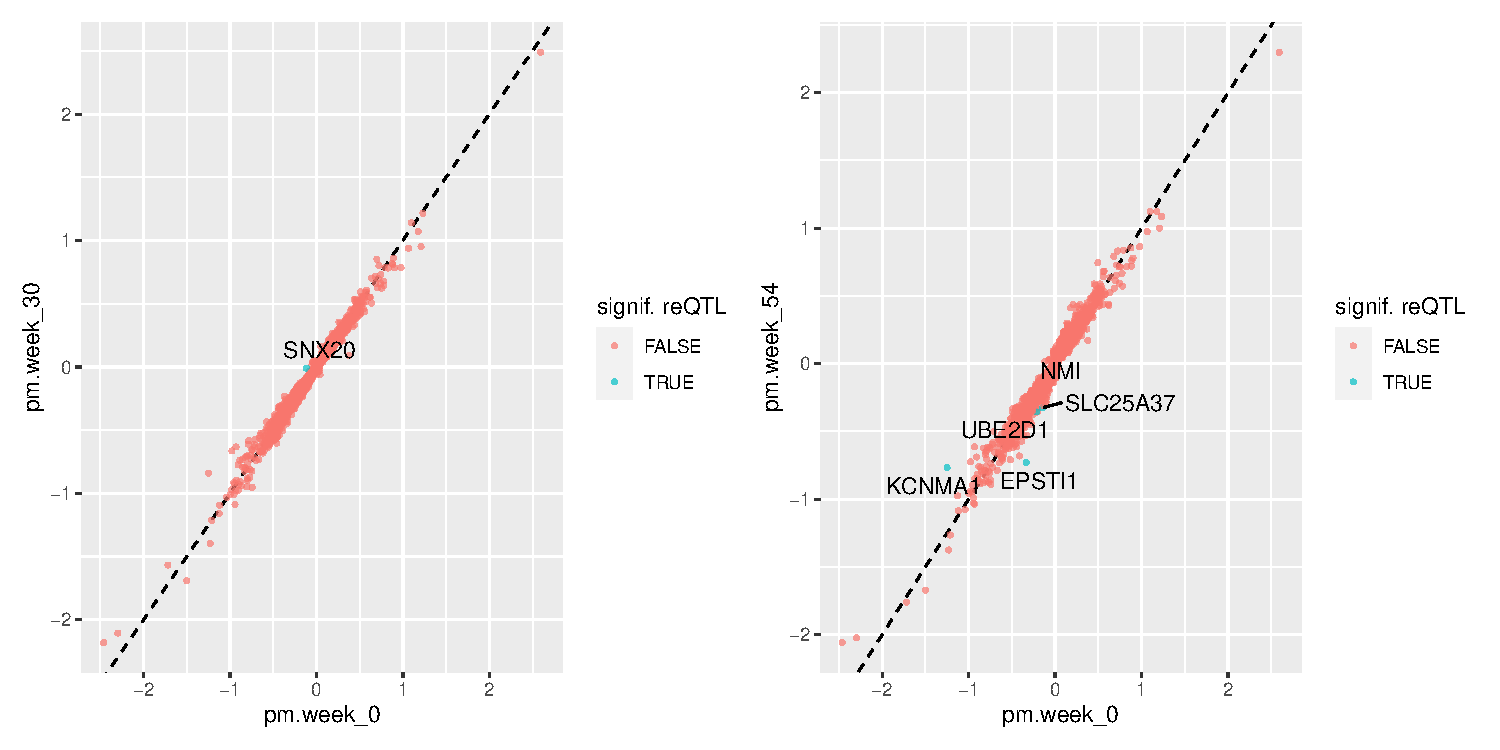
\includegraphics[width=1.0\textwidth,page=1]{mainmatter/figures/chapter_04/plot_dge_eqtl.pm_w30_vs_w0_and_w54_vs_w0}
    \caption{
        \textbf{Week 30 and week 54 eQTL effect sizes vs baseline.}
        Significant reQTLs at FDR 0.05 are labelled.
    }
    \label{fig:multipants_reQTL_pm_w30_vs_w0_and_w54_vs_w0}
\end{figure}

% \1 clustering of eQTL effect sizes across 4 timepoints to identify general patterns of change in beta \todo{similar to the idea of moving from single gene to gene set analyses for more sensitivity}
%     \2 start with prefilter for any reQTL significant at nominal p < 0.05. There were 344.
%         \3 327/344 significant in all timepoints
%     \2 3 main clusters: high effect at w54, high effect at w0 and intermediate cluster (\cref{fig:multipants_reQTL_clusters})
%         \3 ADCY3 is in cluster 3
%     \2 GSEA on cluster 1 revealed enrichment of genes with interferon regulatory motifs in cluster 1 (\cref{fig:multipants_reQTL_clusters_gprofiler})
%     \2 2 INF genes: NMI EPSTI1

% \begin{figure}
%     \centering
%     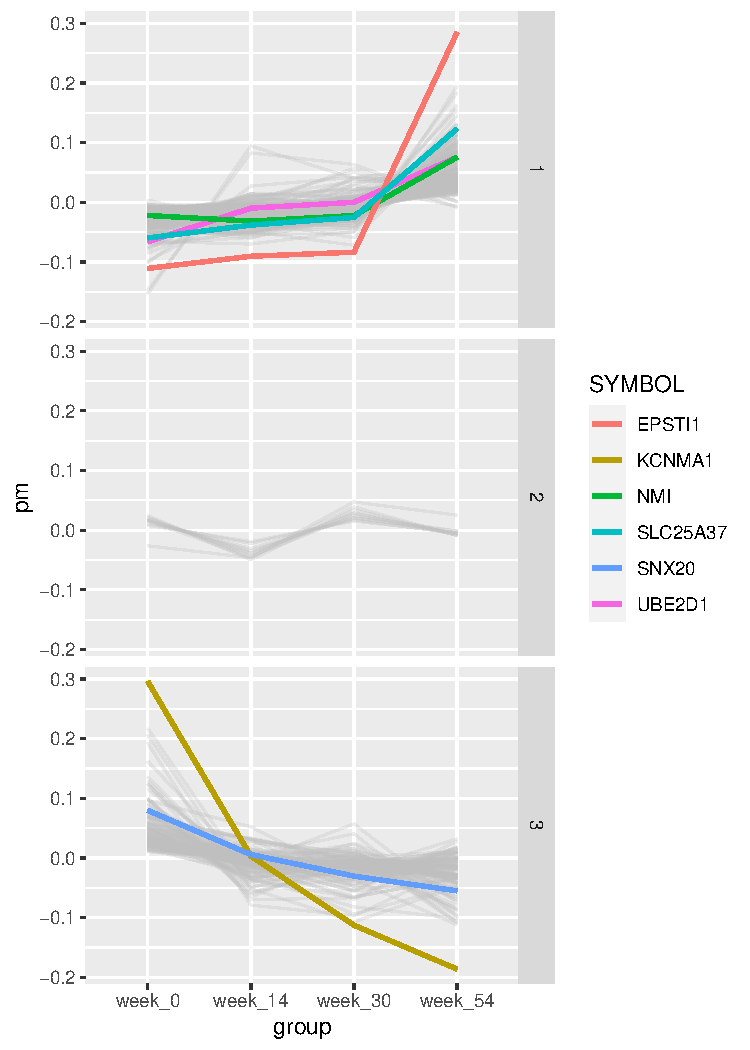
\includegraphics[width=1.0\textwidth,page=1]{mainmatter/figures/chapter_04/plot_dge_eqtl.reQTL_clusters.pdf}
%     \caption{Clustering of eQTL betas over the 4 visits}
%     \label{fig:multipants_reQTL_clusters}
% \end{figure}

% \begin{figure}
%     \centering
%     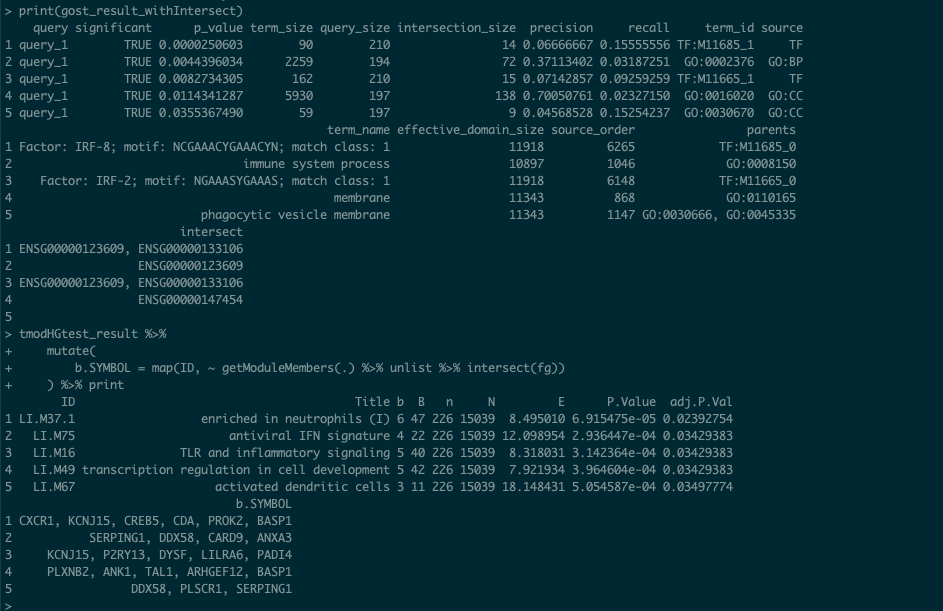
\includegraphics[width=1.0\textwidth,page=1]{mainmatter/figures/chapter_04/reQTL_cluster_1_gene_sets_Screenshot 2020-09-04 at 00.18.57.png}
%     \caption{gene set enrichment using gprofileR for cluster 1 genes}
%     \label{fig:multipants_reQTL_clusters_gprofiler}
% \end{figure}

\section{Discussion}

In \gls{PANTS}, a cohort of \gls{CD} patients receiving infliximab or adalimumab anti-TNF therapy for the first time,
there were substantial differences in whole blood gene expression between primary responders and non-responders.
At baseline, the greatest differences in expression were observed between future responders and non-responders to infliximab,
with increased expression of monocyte, neutrophil and dendritic cell gene modules in responders,
and decreased expression of T cell and NK cell modules.
% \todo{So many modules associations here, maybe try to Google some of them...}
These effects appear to be infliximab-specific, and are attenuated after adjusting for the proportions of six major immune cell types,
suggesting expression differences may be driven by mediation via the proportions of these cell types.
% Although the sample size for infliximab is greater than for adalimumab,
% this is unlikely to be the only factor, as the drugs are much more comparable after adjusting for cell composition.

In contrast, future responders to adalimumab had lower baseline expression of plasma cell and cell division modules.
The module-level results line up with the three per-gene hits for the adalimumab-only analysis:
\gene{IGKV1-9} encodes the immunoglobulin light chain variable region that forms part of antibodies produced by plasma cells,
\gene{KCNN3} is annotated to plasma cell surface signature module (LI.S3 \autocite{li2013MolecularSignaturesAntibody}), 
and the expression of both \gene{KCNN3} and \gene{PDIA5} are correlated with blood plasmablast frequencies \autocite{tsang2014GlobalAnalysesHuman}.
It was reported by \textcite{gaujoux2019CellcentredMetaanalysisReveals} that baseline plasma cell abundances are lower for infliximab responders,
hypothesising that plasma cell survival is supported by increased \gls{TNF} levels in non-responders.
Plasma cells also formed a part of a correlated module of cell populations identified by \autocite{martin2019SingleCellAnalysisCrohn},
where lower module expression was associated with better response to anti-\gls{TNF} in a cohort with patients taking both infliximab and adalimumab.
However, both these studies were conducted in gut biopsy samples, and there was no mention of strong between-drug heterogeneity.

The adalimumab-specific associations I found were more significant after cell proportion adjustment, 
which may indicate per-cell downregulation rather than cell abundance being associated with response.
However, cell composition differences mediated by rarer cell types that have abundances poorly captured by the six major types used in the model will be poorly adjusted for.
For example, plasma cell proportions are only weakly correlated with other immune cell types in the healthy immune system \autocite{zalocusky201810000Immunomes}, 
although the relationship may differ for \gls{CD} patients.
It has also been shown that differentially expressed genes in blood with correction for only common cell types will 
identify associations that are proxies for rare cell types \autocite{pellegrinocoppola2020CorrectionBothCommon}.
If this is the case, the role of the cell composition estimates for adalimumab-specific effects may be more akin to precision variables, 
which would be consistent with increased significance after adjusting.
% although formal tests for difference in effect between adjusted and non-adjusted estimates would be required to confirm this.

The differences between drugs are puzzling, especially the greater effect of cell composition adjustment for infliximab. 
Baseline patient differences between drugs may offer a partial explanation.
% Due to lack of randomisation, patients that took infliximab and adalimumab are likely to differ by more than drug (baseline confounding).
There may be characteristics not listed in \cref{tab:multipants_table1} that differ between patients on different drugs \autocite{kennedy2019PredictorsAntiTNFTreatment}.
% “Several baseline characteristics were significantly different between the infliximab-treated and adalimumab-treated patients, including age, smoking, body-mass index, disease duration, disease location, and disease behaviour. Patients treated with infliximab had more active disease at baseline than did patients treated with adalimumab, as evidenced by higher serum CRP and faecal calprotectin concentrations (table 1).” \autocite{kennedy2019PredictorsAntiTNFTreatment}
In the full \gls{PANTS} cohort, lower albumin, higher \gls{CRP}, and higher faecal calprotectin in infliximab patients suggest that they may have had greater disease severity.
% Nick: “In general, sicker patients have often been given infliximab. At the time, children were rarely given adalimumab, but that doesn’t affect the RNA seq cohort because children were excluded.”
Differences may be driven by patient or physician preference, for example, patients with more severe disease are often given infliximab rather than adalimumab\footnote{Kennedy, N. A., personal communication, 4 June (2020).}.
I have not yet been able to access clinical variables such as \gls{CRP} and faecal calprotectin levels to consider as variables to adjust for in my modelling.
A richer phenotype dataset containing some of these variables has been requested from collaborators.

The strongest single-gene association in the pooled analysis was \gene{SIGLEC10}, 
which had reduced significance post-adjustment with a comparable effect size,
where baseline expression was approximately 25\% higher in responders.
Direction of effect was consistent between drugs, but most significant in infliximab without cell composition adjustment.
In \gls{IBD}, small molecules called \glspl{DAMP} are released due to tissue damage and cell death, 
and further promote inflammation through pathogen sensing \gls{PRR} pathways that include \gls{TLR} family receptors \autocite{boyapati2016GutMucosalDAMPs,desouza2016ImmunopathogenesisIBDCurrent}.
For instance, faecal calprotectin, a marker for \gls{IBD} activity, is a complex of two \glspl{DAMP}, S100A8 and S100A9 \autocite{desouza2016ImmunopathogenesisIBDCurrent}.
SIGLEC10 has been shown to repress \gls{DAMP}-mediated inflammation through binding CD24 \autocite{boyapati2016GutMucosalDAMPs}.
\gene{SIGLEC10} is expressed on B cells, monocytes and eosinophils \autocite{crocker2007SiglecsTheirRoles},
and of these cell types, module level results posit monocytes as the most likely candidate cell type to have increased module expression in responders.
In monocytes, \gene{SIGLEC10} expression is more specific to the CD16+ monocytes \autocite{martinez2009TranscriptomeHumanMonocyte},
and in particular the CD14+CD16++ non-classical monocytes rather than the classical CD14++CD16- or intermediate CD14++CD16+ subsets \autocite{villani2017SinglecellRNAseqReveals}.
% Non-classical (anti-inflammatory) monocytes have a role in many chronic inflam diseases \url{https://www.annualreviews.org/doi/full/10.1146/annurev-immunol-042617-053119#_i16} 
% including CD \url{https://www.researchgate.net/profile/Siew-Cheng_Wong/publication/221723208_The_three_human_monocyte_subsets_Implications_for_health_and_disease/links/09e415101253562a3c000000.pdf}
% Also from above: "The two main forms of human inflammatory boweldiseases (IBD) are Crohn’s disease (CD) and ulcerative colitis (UC), and the expansion of CD16+ monocytes had been reported in both forms of IBD [87,88]. In CD, it is during active disease that the monocyte subsets perturbation was observed [87,89]."
In \gls{PANTS}, it was suggested by \textcite{kennedy2019PredictorsAntiTNFTreatment} that higher inflammatory load as indicated by low baseline albumin levels 
may result in low week 14 drug levels due to faster drug clearance,
and low drug levels at week 14 were in turn associated with non-response.
A hypothetical model might be high baseline \gene{SIGLEC10} expression reflecting 
higher proportions of CD16+ monocytes (or lower proportions of CD16- monocytes),
decreased \gls{DAMP}-mediated inflammation, 
and increased chance of primary response, possibly by affecting drug clearance rate.
This is an extremely tentative model:
both the cell proportion estimates and module definitions used thus far only represent monocytes as a whole,
lacking the resolution to properly explore shifts in the three monocyte subsets.
It may be possible to use expression of monocyte subset marker genes such as those identified by \textcite{villani2017SinglecellRNAseqReveals} to improve the resolution of the cell proportion estimates.

Despite the strong heterogeneity in effects between drugs, one consistent effect that emerged after adjusting for cell composition was 
baseline upregulation of MHC-TLR7-TLR8, antigen presentation, and interferon modules in responders.
% \todo{How does the MHC come in here?}
As mentioned above, \gls{TLR} receptors are involved in pathogen sensing, and TLR7 and TLR8 are endosomal proteins primarily expressed in monocytes, macrophages and \glspl{DC},
part of an antigen presentation pathway that senses bacterial DNA and activates downstream innate immune pathways including type I interferon response \autocite{cervantes2012TLR8ForgottenRelative}.
Type I interferons have pathogenic or protective roles in many \glspl{IMID} \autocite{ivashkiv2014RegulationTypeInterferon}.
It has been suggested that type I interferon responses induced via TLR7 and TLR8 can suppress colitis in mouse models, and play a role in maintaining gut homeostasis \autocite{lu2018TolllikeReceptorsInflammatory,corridoni2018EmergingMechanismsInnate},
so upregulation here may again represent a less severe baseline disease in future responders.
% TODO: what about the main IFN flip result then?
% see "Expression of these genes was higher in responders at week 0 and lower at all post-treatment timepoints."
%
% TODO
% https://www.nature.com/articles/s41467-018-07841-3
% Interestingly, Oncostatim M (OSM21) and TREM122 previously associated with anti-TNF response were within our corticosteroid response gene signature (Fig. 4g), and this signature PC1 showed a high correlation with OSM and TREM1 (0.79 and 0.89, P < 0.0001). We also noted a substantial overlap between the genes from the PROTECT corticosteroid response gene signature and previously described anti-TNF response genes21 (Fig. 4g).
% ...
% Notably, the corticosteroid response gene signature showed a substantial overlap with genes previously associated with anti-TNF response, and exhibited a similar difference between responders and nonresponders to anti-TNF or anti-integrin α4β7 therapies. These similarities support an emerging concept in the field that the mucosal inflammatory state as measured by gene expression may better define the likelihood of response to current treatment approaches than conventional clinical measures of severity.

Most previously reported baseline markers in blood and gut biopsies were non-significant in this study.
% One exception is \gene{PTGS2}, which is also specific to Mono3 in \textcite{villani2017SinglecellRNAseqReveals}.
For gut markers, this may not be unexpected.
Although a subset of gut infiltrating immune cells and their precursors may also be circulating,
genes specific to epithelium and immune cell types that differentiate after they migrate into tissues (e.g. monocyte-derived macrophages),
will be difficult to observe in blood.
For blood markers, I sought to clarify the conflicting results in the literature about the association of \gene{TREM1} expression in blood with anti-\gls{TNF} response \autocite{gaujoux2019CellcentredMetaanalysisReveals,verstockt2019LowTREM1Expression}.
I did not find \gene{TREM1} to be significantly differentially expressed in \gls{PANTS},
although the direction of effect is increased expression in responders,
matching the \textcite{gaujoux2019CellcentredMetaanalysisReveals} direction of effect in blood.
\gene{TREM1} is expressed on myeloid lineage cells such as monocytes and macrophages;
\textcite{villani2017SinglecellRNAseqReveals} reported that \gene{TREM1} expression is most specific to 
classical monocytes and a newly identified subtype within the intermediate monocytes (\enquote{Mono3}).
The \gene{TREM1} effect is one of the infliximab-specific differentially expressed genes that is much stronger without cell proportion adjustment,
so it may reflect association of baseline monocyte cell proportions with response.

There are many factors could explain failures to replicate reported markers, or identification of different markers from study to study.
Many existing studies pool cohorts with different anti-\gls{TNF} biologics due to the scarcity of large datasets,
yet even within this study, there is heterogeneity between drugs.
There are between-study differences in the definition of primary response,
such as endoscopic healing \autocite{gaujoux2019CellcentredMetaanalysisReveals} versus scoring on clinical parameters \autocite{verstockt2019LowTREM1Expression}.
Any two studies are unlikely to have adjusted for the same combinations of covariates in modelling,
and some covariates like cell composition are very influential for bulk expression data.
Finally, small sample sizes have considerable sampling error.
Set-based association tests that draw on changes in multiple genes,
% such as the cell abundance module associations reported for gut biospies by \textcite{martin2019SingleCellAnalysisCrohn},
such as the expression module associations for blood in this study,
may be more reproducible compared to single-gene markers. 
% TODO: TREM1 look at the drug level achievement argument from verstockt

Although this study is purely descriptive, a future aim will be to see if the identified baseline module associations also imply that response status can be predicted from baseline expression.
% Correction for cell proportions has thus far provided complementary interpretations of total effect and effects not mediated by cell count.
Because modules associated with response appear to be mediated by cell proportions,
much of the predictive ability may also lie in differences in cell proportions between responders and non-responders.
% Adjusting would be counterproductive.
Indeed, \textcite{gaujoux2019CellcentredMetaanalysisReveals} noted that adjusting expression for cell composition resulted in gut gene signatures that were worse at discriminating responders from non-responders.
Testing specific subpopulations such as CD16+ monocyte or plasma cell abundance for association with response
can also be viewed as a type of set-based test that represents a set of cell-type specific genes,
and thus may also be more reproducible than single-gene markers.

% Stronger signal to noise ratio
Much larger proportions of the transcriptome are associated with response after the induction period at week 14.
Module associations
showed downregulation of immune activation, \gls{TLR}, inflammatory, monocyte and neutrophil modules in responders;
and upregulation of B and T cell modules.
Similar module associations were also found when considering modules differentially expressed from week 0 to week 14.
The differences between responders and non-responders at week 14 
were qualitatively similar to the differences pre and post anti-\gls{TNF} induction,
suggesting there may be relatively little change in the transcriptome of non-responders after induction.
Associations were generally consistent between drugs for both the within week 14 and change from week 0 to week 14 analyses,
perhaps because the effect of baseline differences between patients taking different drugs on the transcriptome is diluted
by the large transcriptomic perturbation caused by taking an anti-\gls{TNF} drug.
Many of the same modules were also significant regardless of cell proportion correction.

There appears to be a general reduction in immune activation in responders at week 14,
presumably due to successful inhibition of \gls{TNF} by the anti-\gls{TNF} drug,
which is consistent with reduced neutrophil activation and reduced monocyte recruitment \autocite{pramekumar2018PartnersCrimeNeutrophils}.
Apoptosis of monocytes induced by anti-\gls{TNF} in \gls{CD} patients has also been previously observed \autocite{lugering2001InfliximabInducesApoptosis}.
Certain B cell subsets are reduced in the blood of \gls{IBD} patients compared to controls \autocite{pararasa2019ReducedCD27IgDCells}, 
so upregulation of B cell modules after treatment may represent a shift towards health.
Another potential explanation would be increased immunogenicity due to higher drug levels in responders \autocite{kennedy2019PredictorsAntiTNFTreatment}.
Although lack of between-drug heterogeneity does not support the greater immunogenicity of infliximab versus adalimumab.
Overall, it is difficult to determine exact mechanisms in this observational study design, with bulk expression data, using such broad module definitions.

Some previously identified baseline gut markers of response that were not differentially expressed in blood at week 0, were differentially expressed at week 14.
\gene{S100A8} and \gene{S100A9}, identified as markers by \textcite{arijs2010PredictiveValueEpithelial}, which encode components of the inflammatory marker \gls{CRP}, were downregulated in week 14 responders.
The cytokine \gene{OSM}, which promotes inflammation in gut stromal cells \autocite{west2017OncostatinDrivesIntestinal}, was similarly downregulated.
Although it is pointless to use a week 14 marker to predict a response that is defined at week 14,
this does demonstrate that gut markers can coincide with blood markers if expressed in immune cells present in both tissues.

When considering the interaction between change from week 0 to week 14 and response,
the general pattern is magnification in responders,
where the same expression changes occur with greater magnitude than in non-responders.
A potential hypothesis is a continuum of response from non-response to response.
\textcite{gaujoux2019CellcentredMetaanalysisReveals} found changes in cell proportions in response to anti-\gls{TNF} treatment were magnified in responders, 
also supporting response as continuous phenotype.
This study confirms a similar trend at the transcriptional level.

% \1 PNR definition
%     \2 its a very complex binary, but certainly useful
%         \3 kennedy2019PredictorsAntiTNFTreatment Univariable analysis showed, for both drugs, that the most significant determinant of non-remission at week 54 was clinical status at week 14 (table 4; appendix pp 21–22).
%         \3 DGE analysis also agrees with kennedy2019PredictorsAntiTNFTreatment: once PNR, no point in continuing
%     \2 if continuum of PNR? perhaps model decomposed pheno?
%         \3 e.g. "Genetic Loci associated with C-reactive protein levels and risk of coronary heart disease."
%         \3 take advantage of richness of dataset
%     \2 although other mediators of NR could be modelled using genetic instruments e.g drug level

There were some rare exceptions to magnification for genes and modules in the type I interferon pathway.
These showed upregulation in non-responders from week 0 to week 14,
yet were either downregulated or not significantly different for responders.
Single-gene examples include the interferon-induced guanylate-binding proteins \gene{GBP2} and \gene{GBP5} \autocite{tretina2019InterferoninducedGuanylatebindingProteins}, 
and \gene{STAT2}, a key transcription factor for interferon-stimulated genes \autocite{schneider2014InterferonStimulatedGenesComplex}.
Genes such as \gene{IFIT3} and \gene{STAT2} are more strongly induced by type I interferons compared to type II \autocite{liu2012SystematicIdentificationType}.
A study of \gls{RA},
an \gls{IMID} also treated with anti-\gls{TNF} drugs,
also found increases in type I interferon-regulated gene expression in blood after infliximab treatment associated with poor clinical response \autocite{vanbaarsen2010RegulationIFNResponse}.

A spline model of expression over all four timepoints confirmed the above observations made in week 0 and week 14 samples.
% TODO: add KREMEN1 plot
% \todo{then move some of this to results section}
Two main clusters of genes (clusters 1 and 5) contained mostly genes significantly associated with response in the two pairwise comparisons: within week 14, and change from week 0 to week 14.
An example is the most significant single-gene association from the cluster 1 in spline model, \gene{KREMEN1}, 
which was also among most significant associations in the pairwise comparisons.
\gene{KREMEN1} is part of an inflammatory apoptotic pathway in gut epithelium \autocite{laukoetter2008O014IFNGammaInduces}, 
and is downregulated in responders post-induction.
The trajectories of expression for genes in clusters 1 and 5 confirmed changes in expression post-induction were generally greater for responders.
and in addition demonstrates that post-induction expression differences between responders and non-responders are sustained
in samples taken around week 30 and week 54 during the anti-\gls{TNF} maintenance period.
% TODO: does this repeat the results section?
In \gls{PANTS}, \enquote{continuing standard dosing regimens after primary non-response was rarely helpful} for inducing remission by week 54 \autocite{kennedy2019PredictorsAntiTNFTreatment}.
This phenomenon may have a transcriptomic basis,
but non-responders in the \gls{PANTS} \gls{RNAseq} data were selected to exclude patients in remission by week 54,
so trajectories for non-responders at week 14 that eventually achieved remission could not be observed.
% \textcite{gaujoux2019CellcentredMetaanalysisReveals} suggesting increased drug doses may be effective in treating a non-responsive individual.

Making use of data from later timepoints allowed more subtle effects to be detected in the spline analysis.
Clusters 2 and 4 are enriched for B cell genes that were not significantly different at the single-gene level in the within week 0 comparison,
although some downregulation of B cell and plasma cell modules were detected.
% AL353807.3
% STAT1
% BATF2
% GBP1
% GBP5
% IRF1
% TAP1
% APOL2
% APOL1
Cluster 3 reproduced the observation that interferon-induced genes have opposing trajectories of expression in responders and non-responders.
Expression of these genes was higher in responders at week 0 and lower at all post-treatment timepoints.
Here, the cluster contains genes such as \gene{STAT1}, \gene{IRF1} and \gene{TAP1} that are induced by both type I and type II interferons \autocite{liu2012SystematicIdentificationType}.
% TODO: add TREM1 plot
I propose that blood expression of interferon-related genes is an attractive target for future studies of the biological basis of anti-\gls{TNF} response,
or prediction of primary response status.
% If one assumes the model where response and non-response lie along a phenotypic continuum,
% it may be less likely that the opposing directions of regulation can be explained by unmodelled variables such as serum drug level being higher in responders.
% Or indeed TNF being lower in responders.
% \todo{not entirely sure this this is statistically rigorous due to third var effects?}
Since the difference is maintained until week 54, by which time patients would have received many doses of drug,
it is also more likely that response is due to some biological property of an individual patient.
Studies of anti-\gls{TNF} response in \gls{RA} patients have also 
found high baseline interferon activity in blood to be associated with good clinical response \autocite{mavragani2010AssociationResponseTumor,wright2015InterferonGeneExpression}.
%
It should be noted that the number of clusters is only the optimal number determined in this dataset,
and does not imply that genes in different clusters represent biologically distinct pathways.
Clusters 2 and 4 have similar trajectories and enrichments for B cell genes,
and interferon pathway genes appear in both clusters 1 and 3.
% Repeating the analysis setting a different number of clusters, or with bootstrapping, will help to determine a robust number of clusters.

% \1 reQTL mapping to identify changes in genetic control of expression over the timepoints
%     \2 only 6 reQTLs at per-comparison FDR 0.05
%     \2 2 main patterns of reQTLs over time
%     \2 change from baseline expected, but no enrichments
%     \2 but can only speculate on why INF-stimulated genes had change in E from baseline to w54 genetically controlled
%     \2 biases?
%         \3 winner's curse caused by combo of low power and a signif threshold?
%         TODO
%         \3 EE vs EZ model with varying sample size?  https://stephenslab.github.io/mash-application-immune/
%         If we define the reQTL as different standardized effects, the result is EZ V1 model reQTL.
%     \2 vs ch3 HIRD, fewer strong reqtls
%         \3 probably due to low signal: less changes in cell comp across timepoints? or different FDR?
%         \3 and high noise: variation in time since last dose, and much longer timeframe (weeks between doses, vs days since vacc) overall, so more chance for env factors to act
% since E is diff between R and NR,
%     why not put in an interaction between R and NR? not sure if powered
%     not sure if estmating the interaction effect would require more power
%     than losing the averaging effect
Finally, I also attempted to determine if there were changes in genetic architecture of expression over time,
which could indicate that expression response to anti-\gls{TNF} has a genetic component.
Out of all significant lead \glspl{eQTL} for 11156 genes, only six \glspl{reQTL} were detected between baseline and any one of the three post-treatment timepoints.
Although no enrichment analyses are reported due to the small number of associations, 
\gene{NMI} and \gene{EPSTI1} are both interferon-induced genes with significant \glspl{reQTL} that have their strongest effect size on expression at week 54.
Given the issues with doing this \gls{reQTL} analysis in bulk expression data are similar to those encountered in \cref{ch:hird_reQTL},
I did not place emphasis on interpreting these small numbers of associations.
I would also like to verify that these significant \glspl{reQTL} are not artifacts from shrinkage of effect sizes in the joint \gls{eQTL} model,
as their posterior effect sizes from \software{mashr} were very different from the inputs from the timepoint-stratified models.
If these hits are indeed reproducible by complementary methods such as \gls{ASE} \autocite{gutierrez-arcelus2020AllelespecificExpressionChanges},
it may then be worth introducing genotype-response interaction terms in the \gls{eQTL} models
to prioritise \glspl{eQTL} with differing effects in responders and non-responders.
% TODO: would need to change out PEER, which would reduce power to detect eQTLs in the first place
% It would still be difficult to determine cell types responsible
Given there is prior interest in the interferon pathway from \gls{DGE} analyses,
a more statistically powerful approach may be to generate a continuous interferon pathway score for each sample,
which would then act as the interacting variable,
similar to the approach of \textcite{davenport2018DiscoveringVivoCytokineeQTL}.

Several threats to the validity of the study remain to be discussed.
The most pressing may be the meaning of time in the study.
% TODO 
% An alternative option would be to continue to treat timepoint as categorical, then f test all interactions, ignoring variation in study day within timepoints.
% Which may actually be a good thing, since only up to 7 days before next dose.
% Study day does not map to expression well when the time is so long.
% Might be overall more sensible for only 4 timepoints.
For pairwise \gls{DGE} comparisons, expression trajectory clustering, and \gls{reQTL} mapping, 
samples were divided into four timepoints that corresponded to the major visits in \gls{PANTS}.
The \gls{DGE} spline model was fit to study day directly.
Study day has substantial variation around the target for later timepoints.
The particular targets (weeks 14, 30, 54) for post-baseline samples were chosen so that patients on infliximab (8 weeks between doses) and adalimumab (2 weeks between doses) could both be sampled with the same visit structure.
Drug levels peak sharply after each dose and decline exponentially over time.
Visits were scheduled to be as close as possible (within a week) to the next scheduled drug dose to capture trough drug levels.
Neither approach is perfect, as matching patients by timepoint and study day are only attempts to gather samples matched by trough drug level.

% "A LOR visit should be scheduled any time after week 14 if the LOR criteria are met (page 11) and the patient’s gastroenterologist has escalated steroid, immunomodulatory or anti-TNF therapy. Escalation of anti-TNF therapy includes an increase in the dose, or a shortening of the interval between doses."
A further complication is the inclusion of \gls{LOR} samples in analyses.
One treatment option after \gls{LOR} is dose escalation, which may raise trough drug levels for all subsequent visits for those patients.
However, since the \gls{PANTS} protocol allows for \gls{LOR} visits that coincide with major visits to be labelled as a major visit,
there is no guarantee that simply excluding samples labelled as \gls{LOR} would resolve this.
% TODO:
% A worst case hypothetical: assume that there are many more LOR samples in the PR group, since PNR precludes LOR. Differences observed between PR and PNR could just be due to dosing.
%
The best solution may to explicitly model measured serum drug levels as a covariate, where like cell proportions, it would likely act as a mediator of some associations with response.
% Overall 319/840 missing corresponding drug levels.
I did not do this as data missingness would reduce the sample size by about 40\% in this study.
Finding a suitable normalisation of drug level for use in pooled drug analyses is also challenging.
Infliximab and adalimumab have differing pharmokinetics: infliximab has higher peak concentrations, higher peak-trough ratios, and shorter half-life.
The same serum concentrations of infliximab and adalimumab also have different biological effects due to differing therapeutic windows
 \autocite{tracey2008TumorNecrosisFactor,lichtenstein2013ComprehensiveReviewAntitumor,gibson2020ReviewArticleDetermination}.

The effects of differential drop out in responders and non-responders has also not been explored.
% https://rpsychologist.com/lmm-slope-missingness
% Why linear mixed-effects models are probably not the solution to your missing data problems
% https://stats.stackexchange.com/questions/354279/can-a-linear-mixed-model-handle-missing-data-that-is-not-missing-at-random
% As you say, linear mixed-effects (LME) models are assuming that any missing data are missing at random (MAR). A way to account for suspected violations of the MAR assumption of LME models is to use joint models. Under this framework, the longitudinal response and the survival probability are associated by jointly estimating a single likelihood function. Using a joint model, you can get an estimate of how much a possible difference in survival is affecting the longitudinal response and how much the fluctuations in the longitudinal response are associated with survival.
The three main mechanisms of missing data are:
\gls{MCAR}, probability of data being missing is independent of both observed and missing data;
\gls{MAR}, probability of data being missing conditional on observed data is independent of missing data;
and \gls{MNAR}, probability of data being missing depends on missing data \autocite{liu2016MethodsHandlingMissing}.
Even conditional on response status, it is more likely that expression data from more extreme non-responders is missing for later timepoints, so the likely mechanism here is \gls{MNAR},
and the linear mixed models used in this study may be biased.
If it is indeed the most extreme non-responders dropping out, the estimation of responder versus non-responder effects may be conservative in the spline analysis.
% Fortunately, there should be less missingness at weeks 0 and 14.
Note there is no sidestepping a \gls{MNAR} mechanism by analysing only the complete cases, 
since they will differ systematically from the sample as a whole \autocite{ibrahim2009MissingDataMethods}.

% TODO: add a whilst we were not able to X in the intro, the field has advanced by Y, future Z needed
In conclusion,
it remains unclear whether there are any robust single-gene markers for anti-\gls{TNF} response in baseline whole blood of \gls{CD} patients.
Baseline module associations were observed, but there was unexpected heterogeneity between infliximab and adalimumab patients,
so it remains to be seen if such associations will be replicated in separate cohorts.
% TODO: what is in the IBD BioResource? 5.3 Extending anti-TNF pharmacogenetic analysis from alex's thesis
Large upcoming datasets with drug response phenotypes such as the 1000IBD project \autocite{imhann20191000IBDProjectMultiomics} will be invaluable for attempted replication of the associations found in \gls{PANTS}.
Expression differences between responders and non-responders were more distinct at timepoints after the induction period.
I found type I interferon genes went against the general trend of greater transcriptomic change from baseline in responders,
being more upregulated post-treatment in non-responders.
Given the type I interferon expression in blood has also been associated with anti-\gls{TNF} response in \gls{RA} patients,
there may be an opportunity to consider the shared biology of anti-\gls{TNF} response in \gls{IBD} and \gls{RA}.
% and other \glspl{IMID} treated with anti-\gls{TNF} drugs.
Much work has been done generating and validating signatures for anti-\gls{TNF} response in \gls{RA} \autocite{toonen2012ValidationStudyExisting}; but not much work on validating \gls{RA} signatures in \gls{IBD} cohorts and vice versa.

This chapter has been purely descriptive.
Although there are expression differences at many genes between responders and non-responders,
I do not know which cause non-response,
and which are a consequence of disease reduction in responders.
I have deliberately avoided the term \enquote{signature} in my own results, 
as I have not yet had a chance to assess the predictive capability of associated gene modules.
I also did not find evidence for many strong and interpretable \gls{reQTL} effects over time in whole blood, 
so was unable to form hypotheses on the genetic mechanisms influencing anti-\gls{TNF} response via expression.
However, the presence of \glspl{eQTL} for most genes and the presence of strong differences in expression post-induction may allow testing for causal mechanisms where genotype affects drug response via expression.
Strategies for moving onto both prediction and causal inference will be discussed in \cref{ch:discussion}.
%
